\documentclass[twoside]{book}

% Packages required by doxygen
\usepackage{fixltx2e}
\usepackage{calc}
\usepackage{doxygen}
\usepackage[export]{adjustbox} % also loads graphicx
\usepackage{graphicx}
\usepackage[utf8]{inputenc}
\usepackage{makeidx}
\usepackage{multicol}
\usepackage{multirow}
\PassOptionsToPackage{warn}{textcomp}
\usepackage{textcomp}
\usepackage[nointegrals]{wasysym}
\usepackage[table]{xcolor}

% Font selection
\usepackage[T1]{fontenc}
\usepackage[scaled=.90]{helvet}
\usepackage{courier}
\usepackage{amssymb}
\usepackage{sectsty}
\renewcommand{\familydefault}{\sfdefault}
\allsectionsfont{%
  \fontseries{bc}\selectfont%
  \color{darkgray}%
}
\renewcommand{\DoxyLabelFont}{%
  \fontseries{bc}\selectfont%
  \color{darkgray}%
}
\newcommand{\+}{\discretionary{\mbox{\scriptsize$\hookleftarrow$}}{}{}}

% Page & text layout
\usepackage{geometry}
\geometry{%
  a4paper,%
  top=2.5cm,%
  bottom=2.5cm,%
  left=2.5cm,%
  right=2.5cm%
}
\tolerance=750
\hfuzz=15pt
\hbadness=750
\setlength{\emergencystretch}{15pt}
\setlength{\parindent}{0cm}
\setlength{\parskip}{3ex plus 2ex minus 2ex}
\makeatletter
\renewcommand{\paragraph}{%
  \@startsection{paragraph}{4}{0ex}{-1.0ex}{1.0ex}{%
    \normalfont\normalsize\bfseries\SS@parafont%
  }%
}
\renewcommand{\subparagraph}{%
  \@startsection{subparagraph}{5}{0ex}{-1.0ex}{1.0ex}{%
    \normalfont\normalsize\bfseries\SS@subparafont%
  }%
}
\makeatother

% Headers & footers
\usepackage{fancyhdr}
\pagestyle{fancyplain}
\fancyhead[LE]{\fancyplain{}{\bfseries\thepage}}
\fancyhead[CE]{\fancyplain{}{}}
\fancyhead[RE]{\fancyplain{}{\bfseries\leftmark}}
\fancyhead[LO]{\fancyplain{}{\bfseries\rightmark}}
\fancyhead[CO]{\fancyplain{}{}}
\fancyhead[RO]{\fancyplain{}{\bfseries\thepage}}
\fancyfoot[LE]{\fancyplain{}{}}
\fancyfoot[CE]{\fancyplain{}{}}
\fancyfoot[RE]{\fancyplain{}{\bfseries\scriptsize Generated by Doxygen }}
\fancyfoot[LO]{\fancyplain{}{\bfseries\scriptsize Generated by Doxygen }}
\fancyfoot[CO]{\fancyplain{}{}}
\fancyfoot[RO]{\fancyplain{}{}}
\renewcommand{\footrulewidth}{0.4pt}
\renewcommand{\chaptermark}[1]{%
  \markboth{#1}{}%
}
\renewcommand{\sectionmark}[1]{%
  \markright{\thesection\ #1}%
}

% Indices & bibliography
\usepackage{natbib}
\usepackage[titles]{tocloft}
\setcounter{tocdepth}{3}
\setcounter{secnumdepth}{5}
\makeindex

% Hyperlinks (required, but should be loaded last)
\usepackage{ifpdf}
\ifpdf
  \usepackage[pdftex,pagebackref=true]{hyperref}
\else
  \usepackage[ps2pdf,pagebackref=true]{hyperref}
\fi
\hypersetup{%
  colorlinks=true,%
  linkcolor=blue,%
  citecolor=blue,%
  unicode%
}

% Custom commands
\newcommand{\clearemptydoublepage}{%
  \newpage{\pagestyle{empty}\cleardoublepage}%
}

\usepackage{caption}
\captionsetup{labelsep=space,justification=centering,font={bf},singlelinecheck=off,skip=4pt,position=top}

%===== C O N T E N T S =====

\begin{document}

% Titlepage & ToC
\hypersetup{pageanchor=false,
             bookmarksnumbered=true,
             pdfencoding=unicode
            }
\pagenumbering{roman}
\begin{titlepage}
\vspace*{7cm}
\begin{center}%
{\Large Facebook\+Application \\[1ex]\large 1.\+0 }\\
\vspace*{1cm}
{\large Generated by Doxygen 1.8.11}\\
\end{center}
\end{titlepage}
\clearemptydoublepage
\tableofcontents
\clearemptydoublepage
\pagenumbering{arabic}
\hypersetup{pageanchor=true}

%--- Begin generated contents ---
\chapter{L\+I\+C\+E\+N\+SE}
\label{md_FacebookApplication_packages_Newtonsoft.Json.10.0.3_LICENSE}
\hypertarget{md_FacebookApplication_packages_Newtonsoft.Json.10.0.3_LICENSE}{}
The M\+IT License (M\+IT)

Copyright (c) 2007 James Newton-\/\+King

Permission is hereby granted, free of charge, to any person obtaining a copy of this software and associated documentation files (the \char`\"{}\+Software\char`\"{}), to deal in the Software without restriction, including without limitation the rights to use, copy, modify, merge, publish, distribute, sublicense, and/or sell copies of the Software, and to permit persons to whom the Software is furnished to do so, subject to the following conditions\+:

The above copyright notice and this permission notice shall be included in all copies or substantial portions of the Software.

T\+HE S\+O\+F\+T\+W\+A\+RE IS P\+R\+O\+V\+I\+D\+ED \char`\"{}\+A\+S I\+S\char`\"{}, W\+I\+T\+H\+O\+UT W\+A\+R\+R\+A\+N\+TY OF A\+NY K\+I\+ND, E\+X\+P\+R\+E\+SS OR I\+M\+P\+L\+I\+ED, I\+N\+C\+L\+U\+D\+I\+NG B\+UT N\+OT L\+I\+M\+I\+T\+ED TO T\+HE W\+A\+R\+R\+A\+N\+T\+I\+ES OF M\+E\+R\+C\+H\+A\+N\+T\+A\+B\+I\+L\+I\+TY, F\+I\+T\+N\+E\+SS F\+OR A P\+A\+R\+T\+I\+C\+U\+L\+AR P\+U\+R\+P\+O\+SE A\+ND N\+O\+N\+I\+N\+F\+R\+I\+N\+G\+E\+M\+E\+NT. IN NO E\+V\+E\+NT S\+H\+A\+LL T\+HE A\+U\+T\+H\+O\+RS OR C\+O\+P\+Y\+R\+I\+G\+HT H\+O\+L\+D\+E\+RS BE L\+I\+A\+B\+LE F\+OR A\+NY C\+L\+A\+IM, D\+A\+M\+A\+G\+ES OR O\+T\+H\+ER L\+I\+A\+B\+I\+L\+I\+TY, W\+H\+E\+T\+H\+ER IN AN A\+C\+T\+I\+ON OF C\+O\+N\+T\+R\+A\+CT, T\+O\+RT OR O\+T\+H\+E\+R\+W\+I\+SE, A\+R\+I\+S\+I\+NG F\+R\+OM, O\+UT OF OR IN C\+O\+N\+N\+E\+C\+T\+I\+ON W\+I\+TH T\+HE S\+O\+F\+T\+W\+A\+RE OR T\+HE U\+SE OR O\+T\+H\+ER D\+E\+A\+L\+I\+N\+GS IN T\+HE S\+O\+F\+T\+W\+A\+RE. 
\chapter{Namespace Index}
\section{Packages}
Here are the packages with brief descriptions (if available)\+:\begin{DoxyCompactList}
\item\contentsline{section}{\hyperlink{namespace_client}{Client} }{\pageref{namespace_client}}{}
\item\contentsline{section}{\hyperlink{namespace_data}{Data} }{\pageref{namespace_data}}{}
\item\contentsline{section}{\hyperlink{namespace_data_1_1_facebook_objects}{Data.\+Facebook\+Objects} }{\pageref{namespace_data_1_1_facebook_objects}}{}
\item\contentsline{section}{\hyperlink{namespace_g_u_i}{G\+UI} }{\pageref{namespace_g_u_i}}{}
\item\contentsline{section}{\hyperlink{namespace_main}{Main} }{\pageref{namespace_main}}{}
\item\contentsline{section}{\hyperlink{namespace_operations}{Operations} }{\pageref{namespace_operations}}{}
\item\contentsline{section}{\hyperlink{namespace_operations_1_1_client_operations}{Operations.\+Client\+Operations} }{\pageref{namespace_operations_1_1_client_operations}}{}
\item\contentsline{section}{\hyperlink{namespace_operations_1_1_data_operations}{Operations.\+Data\+Operations} }{\pageref{namespace_operations_1_1_data_operations}}{}
\item\contentsline{section}{\hyperlink{namespace_services}{Services} }{\pageref{namespace_services}}{}
\item\contentsline{section}{\hyperlink{namespace_services_1_1_proxy}{Services.\+Proxy} }{\pageref{namespace_services_1_1_proxy}}{}
\item\contentsline{section}{\hyperlink{namespace_services_1_1_token}{Services.\+Token} }{\pageref{namespace_services_1_1_token}}{}
\item\contentsline{section}{\hyperlink{namespace_stetic}{Stetic} }{\pageref{namespace_stetic}}{}
\end{DoxyCompactList}

\chapter{Hierarchical Index}
\section{Class Hierarchy}
This inheritance list is sorted roughly, but not completely, alphabetically\+:\begin{DoxyCompactList}
\item \contentsline{section}{Data.\+A\+P\+I\+Args}{\pageref{class_data_1_1_a_p_i_args}}{}
\item \contentsline{section}{Data.\+Facebook\+Objects.\+Application}{\pageref{class_data_1_1_facebook_objects_1_1_application}}{}
\item \contentsline{section}{Data.\+Facebook\+Objects.\+Comment}{\pageref{class_data_1_1_facebook_objects_1_1_comment}}{}
\item \contentsline{section}{Data.\+Facebook\+Objects.\+Feed}{\pageref{class_data_1_1_facebook_objects_1_1_feed}}{}
\item \contentsline{section}{Operations.\+Client\+Operations.\+I\+Client\+Get\+Operations}{\pageref{interface_operations_1_1_client_operations_1_1_i_client_get_operations}}{}
\begin{DoxyCompactList}
\item \contentsline{section}{Operations.\+Client\+Operations.\+Client\+Get\+Operations}{\pageref{class_operations_1_1_client_operations_1_1_client_get_operations}}{}
\end{DoxyCompactList}
\item \contentsline{section}{Operations.\+Client\+Operations.\+I\+Client\+Store\+Operations}{\pageref{interface_operations_1_1_client_operations_1_1_i_client_store_operations}}{}
\begin{DoxyCompactList}
\item \contentsline{section}{Operations.\+Client\+Operations.\+Client\+Store\+Operations}{\pageref{class_operations_1_1_client_operations_1_1_client_store_operations}}{}
\end{DoxyCompactList}
\item \contentsline{section}{Client.\+I\+D\+B\+Client}{\pageref{interface_client_1_1_i_d_b_client}}{}
\begin{DoxyCompactList}
\item \contentsline{section}{Client.\+D\+B\+Client}{\pageref{class_client_1_1_d_b_client}}{}
\end{DoxyCompactList}
\item \contentsline{section}{Client.\+I\+Facebook\+Client}{\pageref{interface_client_1_1_i_facebook_client}}{}
\begin{DoxyCompactList}
\item \contentsline{section}{Client.\+Facebook\+Client}{\pageref{class_client_1_1_facebook_client}}{}
\end{DoxyCompactList}
\item \contentsline{section}{Operations.\+Data\+Operations.\+I\+Populate\+N\+E\+T\+Object}{\pageref{interface_operations_1_1_data_operations_1_1_i_populate_n_e_t_object}}{}
\begin{DoxyCompactList}
\item \contentsline{section}{Operations.\+Data\+Operations.\+Populate\+N\+E\+T\+Object}{\pageref{class_operations_1_1_data_operations_1_1_populate_n_e_t_object}}{}
\end{DoxyCompactList}
\item \contentsline{section}{Services.\+I\+Text\+Reader}{\pageref{interface_services_1_1_i_text_reader}}{}
\begin{DoxyCompactList}
\item \contentsline{section}{Services.\+Proxy.\+Proxy\+Information}{\pageref{class_services_1_1_proxy_1_1_proxy_information}}{}
\item \contentsline{section}{Services.\+Token.\+Token\+Information}{\pageref{class_services_1_1_token_1_1_token_information}}{}
\end{DoxyCompactList}
\item \contentsline{section}{G\+U\+I.\+Main\+Class}{\pageref{class_g_u_i_1_1_main_class}}{}
\item \contentsline{section}{Data.\+Facebook\+Objects.\+Post}{\pageref{class_data_1_1_facebook_objects_1_1_post}}{}
\item \contentsline{section}{Main.\+Program}{\pageref{class_main_1_1_program}}{}
\item \contentsline{section}{Data.\+Facebook\+Objects.\+Properties}{\pageref{class_data_1_1_facebook_objects_1_1_properties}}{}
\item Window\begin{DoxyCompactList}
\item \contentsline{section}{Main\+Window}{\pageref{class_main_window}}{}
\end{DoxyCompactList}
\end{DoxyCompactList}

\chapter{Class Index}
\section{Class List}
Here are the classes, structs, unions and interfaces with brief descriptions\+:\begin{DoxyCompactList}
\item\contentsline{section}{\hyperlink{class_data_1_1_a_p_i_args}{Data.\+A\+P\+I\+Args} }{\pageref{class_data_1_1_a_p_i_args}}{}
\item\contentsline{section}{\hyperlink{class_data_1_1_facebook_objects_1_1_application}{Data.\+Facebook\+Objects.\+Application} }{\pageref{class_data_1_1_facebook_objects_1_1_application}}{}
\item\contentsline{section}{\hyperlink{class_operations_1_1_client_operations_1_1_client_get_operations}{Operations.\+Client\+Operations.\+Client\+Get\+Operations} }{\pageref{class_operations_1_1_client_operations_1_1_client_get_operations}}{}
\item\contentsline{section}{\hyperlink{class_operations_1_1_client_operations_1_1_client_store_operations}{Operations.\+Client\+Operations.\+Client\+Store\+Operations} }{\pageref{class_operations_1_1_client_operations_1_1_client_store_operations}}{}
\item\contentsline{section}{\hyperlink{class_data_1_1_facebook_objects_1_1_comment}{Data.\+Facebook\+Objects.\+Comment} }{\pageref{class_data_1_1_facebook_objects_1_1_comment}}{}
\item\contentsline{section}{\hyperlink{class_client_1_1_d_b_client}{Client.\+D\+B\+Client} }{\pageref{class_client_1_1_d_b_client}}{}
\item\contentsline{section}{\hyperlink{class_client_1_1_facebook_client}{Client.\+Facebook\+Client} \\*\hyperlink{class_client_1_1_facebook_client}{Facebook\+Client} Class }{\pageref{class_client_1_1_facebook_client}}{}
\item\contentsline{section}{\hyperlink{class_data_1_1_facebook_objects_1_1_feed}{Data.\+Facebook\+Objects.\+Feed} }{\pageref{class_data_1_1_facebook_objects_1_1_feed}}{}
\item\contentsline{section}{\hyperlink{interface_operations_1_1_client_operations_1_1_i_client_get_operations}{Operations.\+Client\+Operations.\+I\+Client\+Get\+Operations} }{\pageref{interface_operations_1_1_client_operations_1_1_i_client_get_operations}}{}
\item\contentsline{section}{\hyperlink{interface_operations_1_1_client_operations_1_1_i_client_store_operations}{Operations.\+Client\+Operations.\+I\+Client\+Store\+Operations} }{\pageref{interface_operations_1_1_client_operations_1_1_i_client_store_operations}}{}
\item\contentsline{section}{\hyperlink{interface_client_1_1_i_d_b_client}{Client.\+I\+D\+B\+Client} }{\pageref{interface_client_1_1_i_d_b_client}}{}
\item\contentsline{section}{\hyperlink{interface_client_1_1_i_facebook_client}{Client.\+I\+Facebook\+Client} \\*Interface Framework for \hyperlink{class_client_1_1_facebook_client}{Facebook\+Client} }{\pageref{interface_client_1_1_i_facebook_client}}{}
\item\contentsline{section}{\hyperlink{interface_operations_1_1_data_operations_1_1_i_populate_n_e_t_object}{Operations.\+Data\+Operations.\+I\+Populate\+N\+E\+T\+Object} }{\pageref{interface_operations_1_1_data_operations_1_1_i_populate_n_e_t_object}}{}
\item\contentsline{section}{\hyperlink{interface_services_1_1_i_text_reader}{Services.\+I\+Text\+Reader} }{\pageref{interface_services_1_1_i_text_reader}}{}
\item\contentsline{section}{\hyperlink{class_g_u_i_1_1_main_class}{G\+U\+I.\+Main\+Class} }{\pageref{class_g_u_i_1_1_main_class}}{}
\item\contentsline{section}{\hyperlink{class_main_window}{Main\+Window} }{\pageref{class_main_window}}{}
\item\contentsline{section}{\hyperlink{class_operations_1_1_data_operations_1_1_populate_n_e_t_object}{Operations.\+Data\+Operations.\+Populate\+N\+E\+T\+Object} \\*Class with methods for populating custom object-\/types }{\pageref{class_operations_1_1_data_operations_1_1_populate_n_e_t_object}}{}
\item\contentsline{section}{\hyperlink{class_data_1_1_facebook_objects_1_1_post}{Data.\+Facebook\+Objects.\+Post} }{\pageref{class_data_1_1_facebook_objects_1_1_post}}{}
\item\contentsline{section}{\hyperlink{class_main_1_1_program}{Main.\+Program} }{\pageref{class_main_1_1_program}}{}
\item\contentsline{section}{\hyperlink{class_data_1_1_facebook_objects_1_1_properties}{Data.\+Facebook\+Objects.\+Properties} }{\pageref{class_data_1_1_facebook_objects_1_1_properties}}{}
\item\contentsline{section}{\hyperlink{class_services_1_1_proxy_1_1_proxy_information}{Services.\+Proxy.\+Proxy\+Information} }{\pageref{class_services_1_1_proxy_1_1_proxy_information}}{}
\item\contentsline{section}{\hyperlink{class_services_1_1_token_1_1_token_information}{Services.\+Token.\+Token\+Information} }{\pageref{class_services_1_1_token_1_1_token_information}}{}
\end{DoxyCompactList}

\chapter{File Index}
\section{File List}
Here is a list of all files with brief descriptions\+:\begin{DoxyCompactList}
\item\contentsline{section}{Facebook\+Application/\+Client/\hyperlink{_d_b_client_8cs}{D\+B\+Client.\+cs} }{\pageref{_d_b_client_8cs}}{}
\item\contentsline{section}{Facebook\+Application/\+Client/\hyperlink{_facebook_client_8cs}{Facebook\+Client.\+cs} }{\pageref{_facebook_client_8cs}}{}
\item\contentsline{section}{Facebook\+Application/\+Client/\+Properties/\hyperlink{_client_2_properties_2_assembly_info_8cs}{Assembly\+Info.\+cs} }{\pageref{_client_2_properties_2_assembly_info_8cs}}{}
\item\contentsline{section}{Facebook\+Application/\+Data/\hyperlink{_a_p_i_args_8cs}{A\+P\+I\+Args.\+cs} }{\pageref{_a_p_i_args_8cs}}{}
\item\contentsline{section}{Facebook\+Application/\+Data/\+Facebook\+Objects/\hyperlink{_comment_8cs}{Comment.\+cs} }{\pageref{_comment_8cs}}{}
\item\contentsline{section}{Facebook\+Application/\+Data/\+Facebook\+Objects/\hyperlink{_feed_8cs}{Feed.\+cs} }{\pageref{_feed_8cs}}{}
\item\contentsline{section}{Facebook\+Application/\+Data/\+Facebook\+Objects/\hyperlink{_post_8cs}{Post.\+cs} }{\pageref{_post_8cs}}{}
\item\contentsline{section}{Facebook\+Application/\+Data/\+Properties/\hyperlink{_data_2_properties_2_assembly_info_8cs}{Assembly\+Info.\+cs} }{\pageref{_data_2_properties_2_assembly_info_8cs}}{}
\item\contentsline{section}{Facebook\+Application/\+G\+U\+I/\hyperlink{_main_window_8cs}{Main\+Window.\+cs} }{\pageref{_main_window_8cs}}{}
\item\contentsline{section}{Facebook\+Application/\+G\+U\+I/\hyperlink{_g_u_i_2_program_8cs}{Program.\+cs} }{\pageref{_g_u_i_2_program_8cs}}{}
\item\contentsline{section}{Facebook\+Application/\+G\+U\+I/gtk-\/gui/\hyperlink{generated_8cs}{generated.\+cs} }{\pageref{generated_8cs}}{}
\item\contentsline{section}{Facebook\+Application/\+G\+U\+I/gtk-\/gui/\hyperlink{gtk-gui_2_main_window_8cs}{Main\+Window.\+cs} }{\pageref{gtk-gui_2_main_window_8cs}}{}
\item\contentsline{section}{Facebook\+Application/\+G\+U\+I/\+Properties/\hyperlink{_g_u_i_2_properties_2_assembly_info_8cs}{Assembly\+Info.\+cs} }{\pageref{_g_u_i_2_properties_2_assembly_info_8cs}}{}
\item\contentsline{section}{Facebook\+Application/\+Main/\hyperlink{_main_2_program_8cs}{Program.\+cs} }{\pageref{_main_2_program_8cs}}{}
\item\contentsline{section}{Facebook\+Application/\+Operations/\+Client\+Operations/\hyperlink{_client_get_operation_8cs}{Client\+Get\+Operation.\+cs} }{\pageref{_client_get_operation_8cs}}{}
\item\contentsline{section}{Facebook\+Application/\+Operations/\+Client\+Operations/\hyperlink{_client_store_operations_8cs}{Client\+Store\+Operations.\+cs} }{\pageref{_client_store_operations_8cs}}{}
\item\contentsline{section}{Facebook\+Application/\+Operations/\+Data\+Operations/\hyperlink{_populate_n_e_t_object_8cs}{Populate\+N\+E\+T\+Object.\+cs} }{\pageref{_populate_n_e_t_object_8cs}}{}
\item\contentsline{section}{Facebook\+Application/\+Operations/\+Properties/\hyperlink{_operations_2_properties_2_assembly_info_8cs}{Assembly\+Info.\+cs} }{\pageref{_operations_2_properties_2_assembly_info_8cs}}{}
\item\contentsline{section}{Facebook\+Application/\+Services/\hyperlink{_i_text_reader_8cs}{I\+Text\+Reader.\+cs} }{\pageref{_i_text_reader_8cs}}{}
\item\contentsline{section}{Facebook\+Application/\+Services/\+Properties/\hyperlink{_services_2_properties_2_assembly_info_8cs}{Assembly\+Info.\+cs} }{\pageref{_services_2_properties_2_assembly_info_8cs}}{}
\item\contentsline{section}{Facebook\+Application/\+Services/\+Proxy/\hyperlink{_proxy_information_8cs}{Proxy\+Information.\+cs} }{\pageref{_proxy_information_8cs}}{}
\item\contentsline{section}{Facebook\+Application/\+Services/\+Token/\hyperlink{_token_information_8cs}{Token\+Information.\+cs} }{\pageref{_token_information_8cs}}{}
\end{DoxyCompactList}

\chapter{Namespace Documentation}
\hypertarget{namespace_client}{}\section{Client Namespace Reference}
\label{namespace_client}\index{Client@{Client}}
\subsection*{Classes}
\begin{DoxyCompactItemize}
\item 
class \hyperlink{class_client_1_1_d_b_client}{D\+B\+Client}
\item 
class \hyperlink{class_client_1_1_facebook_client}{Facebook\+Client}
\begin{DoxyCompactList}\small\item\em \hyperlink{class_client_1_1_facebook_client}{Facebook\+Client} Class \end{DoxyCompactList}\item 
interface \hyperlink{interface_client_1_1_i_d_b_client}{I\+D\+B\+Client}
\item 
interface \hyperlink{interface_client_1_1_i_facebook_client}{I\+Facebook\+Client}
\begin{DoxyCompactList}\small\item\em Interface Framework for \hyperlink{class_client_1_1_facebook_client}{Facebook\+Client} \end{DoxyCompactList}\end{DoxyCompactItemize}

\hypertarget{namespace_data}{}\section{Data Namespace Reference}
\label{namespace_data}\index{Data@{Data}}
\subsection*{Namespaces}
\begin{DoxyCompactItemize}
\item 
namespace \hyperlink{namespace_data_1_1_facebook_objects}{Facebook\+Objects}
\end{DoxyCompactItemize}
\subsection*{Classes}
\begin{DoxyCompactItemize}
\item 
class \hyperlink{class_data_1_1_a_p_i_args}{A\+P\+I\+Args}
\end{DoxyCompactItemize}

\hypertarget{namespace_data_1_1_facebook_objects}{}\section{Data.\+Facebook\+Objects Namespace Reference}
\label{namespace_data_1_1_facebook_objects}\index{Data.\+Facebook\+Objects@{Data.\+Facebook\+Objects}}
\subsection*{Classes}
\begin{DoxyCompactItemize}
\item 
class \hyperlink{class_data_1_1_facebook_objects_1_1_application}{Application}
\item 
class \hyperlink{class_data_1_1_facebook_objects_1_1_comment}{Comment}
\item 
class \hyperlink{class_data_1_1_facebook_objects_1_1_feed}{Feed}
\item 
class \hyperlink{class_data_1_1_facebook_objects_1_1_post}{Post}
\item 
class \hyperlink{class_data_1_1_facebook_objects_1_1_properties}{Properties}
\end{DoxyCompactItemize}

\hypertarget{namespace_g_u_i}{}\section{G\+UI Namespace Reference}
\label{namespace_g_u_i}\index{G\+UI@{G\+UI}}
\subsection*{Classes}
\begin{DoxyCompactItemize}
\item 
class \hyperlink{class_g_u_i_1_1_main_class}{Main\+Class}
\end{DoxyCompactItemize}

\hypertarget{namespace_main}{}\section{Main Namespace Reference}
\label{namespace_main}\index{Main@{Main}}
\subsection*{Classes}
\begin{DoxyCompactItemize}
\item 
class \hyperlink{class_main_1_1_program}{Program}
\end{DoxyCompactItemize}

\hypertarget{namespace_operations}{}\section{Operations Namespace Reference}
\label{namespace_operations}\index{Operations@{Operations}}
\subsection*{Namespaces}
\begin{DoxyCompactItemize}
\item 
namespace \hyperlink{namespace_operations_1_1_client_operations}{Client\+Operations}
\item 
namespace \hyperlink{namespace_operations_1_1_data_operations}{Data\+Operations}
\end{DoxyCompactItemize}

\hypertarget{namespace_operations_1_1_client_operations}{}\section{Operations.\+Client\+Operations Namespace Reference}
\label{namespace_operations_1_1_client_operations}\index{Operations.\+Client\+Operations@{Operations.\+Client\+Operations}}
\subsection*{Classes}
\begin{DoxyCompactItemize}
\item 
class \hyperlink{class_operations_1_1_client_operations_1_1_client_get_operations}{Client\+Get\+Operations}
\item 
class \hyperlink{class_operations_1_1_client_operations_1_1_client_store_operations}{Client\+Store\+Operations}
\item 
interface \hyperlink{interface_operations_1_1_client_operations_1_1_i_client_get_operations}{I\+Client\+Get\+Operations}
\item 
interface \hyperlink{interface_operations_1_1_client_operations_1_1_i_client_store_operations}{I\+Client\+Store\+Operations}
\end{DoxyCompactItemize}

\hypertarget{namespace_operations_1_1_data_operations}{}\section{Operations.\+Data\+Operations Namespace Reference}
\label{namespace_operations_1_1_data_operations}\index{Operations.\+Data\+Operations@{Operations.\+Data\+Operations}}
\subsection*{Classes}
\begin{DoxyCompactItemize}
\item 
interface \hyperlink{interface_operations_1_1_data_operations_1_1_i_populate_n_e_t_object}{I\+Populate\+N\+E\+T\+Object}
\item 
class \hyperlink{class_operations_1_1_data_operations_1_1_populate_n_e_t_object}{Populate\+N\+E\+T\+Object}
\begin{DoxyCompactList}\small\item\em Class with methods for populating custom object-\/types \end{DoxyCompactList}\end{DoxyCompactItemize}

\hypertarget{namespace_services}{}\section{Services Namespace Reference}
\label{namespace_services}\index{Services@{Services}}
\subsection*{Namespaces}
\begin{DoxyCompactItemize}
\item 
namespace \hyperlink{namespace_services_1_1_proxy}{Proxy}
\item 
namespace \hyperlink{namespace_services_1_1_token}{Token}
\end{DoxyCompactItemize}
\subsection*{Classes}
\begin{DoxyCompactItemize}
\item 
interface \hyperlink{interface_services_1_1_i_text_reader}{I\+Text\+Reader}
\end{DoxyCompactItemize}

\hypertarget{namespace_services_1_1_proxy}{}\section{Services.\+Proxy Namespace Reference}
\label{namespace_services_1_1_proxy}\index{Services.\+Proxy@{Services.\+Proxy}}
\subsection*{Classes}
\begin{DoxyCompactItemize}
\item 
class \hyperlink{class_services_1_1_proxy_1_1_proxy_information}{Proxy\+Information}
\end{DoxyCompactItemize}

\hypertarget{namespace_services_1_1_token}{}\section{Services.\+Token Namespace Reference}
\label{namespace_services_1_1_token}\index{Services.\+Token@{Services.\+Token}}
\subsection*{Classes}
\begin{DoxyCompactItemize}
\item 
class \hyperlink{class_services_1_1_token_1_1_token_information}{Token\+Information}
\end{DoxyCompactItemize}

\hypertarget{namespace_stetic}{}\section{Stetic Namespace Reference}
\label{namespace_stetic}\index{Stetic@{Stetic}}
\subsection*{Classes}
\begin{DoxyCompactItemize}
\item 
class {\bfseries Action\+Groups}
\item 
class {\bfseries Gui}
\end{DoxyCompactItemize}

\chapter{Class Documentation}
\hypertarget{class_data_1_1_a_p_i_args}{}\section{Data.\+A\+P\+I\+Args Class Reference}
\label{class_data_1_1_a_p_i_args}\index{Data.\+A\+P\+I\+Args@{Data.\+A\+P\+I\+Args}}


Collaboration diagram for Data.\+A\+P\+I\+Args\+:
\nopagebreak
\begin{figure}[H]
\begin{center}
\leavevmode
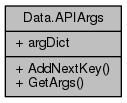
\includegraphics[width=167pt]{class_data_1_1_a_p_i_args__coll__graph}
\end{center}
\end{figure}
\subsection*{Public Member Functions}
\begin{DoxyCompactItemize}
\item 
string \hyperlink{class_data_1_1_a_p_i_args_aee8dceb9797a0fcab0c700f227cea61a}{Add\+Next\+Key} (string arg\+Type, string key)
\item 
string \hyperlink{class_data_1_1_a_p_i_args_a78c8568d1ede724c907a36454dcda88e}{Get\+Args} (string arg\+Type)
\end{DoxyCompactItemize}
\subsection*{Public Attributes}
\begin{DoxyCompactItemize}
\item 
Dictionary$<$ string, string $>$ \hyperlink{class_data_1_1_a_p_i_args_a86541aeaf3d536fa12c75ac1eb404807}{arg\+Dict}
\end{DoxyCompactItemize}


\subsection{Detailed Description}


Definition at line 5 of file A\+P\+I\+Args.\+cs.



\subsection{Member Function Documentation}
\index{Data\+::\+A\+P\+I\+Args@{Data\+::\+A\+P\+I\+Args}!Add\+Next\+Key@{Add\+Next\+Key}}
\index{Add\+Next\+Key@{Add\+Next\+Key}!Data\+::\+A\+P\+I\+Args@{Data\+::\+A\+P\+I\+Args}}
\subsubsection[{\texorpdfstring{Add\+Next\+Key(string arg\+Type, string key)}{AddNextKey(string argType, string key)}}]{\setlength{\rightskip}{0pt plus 5cm}string Data.\+A\+P\+I\+Args.\+Add\+Next\+Key (
\begin{DoxyParamCaption}
\item[{string}]{arg\+Type, }
\item[{string}]{key}
\end{DoxyParamCaption}
)}\hypertarget{class_data_1_1_a_p_i_args_aee8dceb9797a0fcab0c700f227cea61a}{}\label{class_data_1_1_a_p_i_args_aee8dceb9797a0fcab0c700f227cea61a}


Definition at line 35 of file A\+P\+I\+Args.\+cs.

\index{Data\+::\+A\+P\+I\+Args@{Data\+::\+A\+P\+I\+Args}!Get\+Args@{Get\+Args}}
\index{Get\+Args@{Get\+Args}!Data\+::\+A\+P\+I\+Args@{Data\+::\+A\+P\+I\+Args}}
\subsubsection[{\texorpdfstring{Get\+Args(string arg\+Type)}{GetArgs(string argType)}}]{\setlength{\rightskip}{0pt plus 5cm}string Data.\+A\+P\+I\+Args.\+Get\+Args (
\begin{DoxyParamCaption}
\item[{string}]{arg\+Type}
\end{DoxyParamCaption}
)}\hypertarget{class_data_1_1_a_p_i_args_a78c8568d1ede724c907a36454dcda88e}{}\label{class_data_1_1_a_p_i_args_a78c8568d1ede724c907a36454dcda88e}


Definition at line 40 of file A\+P\+I\+Args.\+cs.



Referenced by Main.\+Program.\+Main().



Here is the caller graph for this function\+:
\nopagebreak
\begin{figure}[H]
\begin{center}
\leavevmode
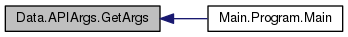
\includegraphics[width=333pt]{class_data_1_1_a_p_i_args_a78c8568d1ede724c907a36454dcda88e_icgraph}
\end{center}
\end{figure}




\subsection{Member Data Documentation}
\index{Data\+::\+A\+P\+I\+Args@{Data\+::\+A\+P\+I\+Args}!arg\+Dict@{arg\+Dict}}
\index{arg\+Dict@{arg\+Dict}!Data\+::\+A\+P\+I\+Args@{Data\+::\+A\+P\+I\+Args}}
\subsubsection[{\texorpdfstring{arg\+Dict}{argDict}}]{\setlength{\rightskip}{0pt plus 5cm}Dictionary$<$string, string$>$ Data.\+A\+P\+I\+Args.\+arg\+Dict}\hypertarget{class_data_1_1_a_p_i_args_a86541aeaf3d536fa12c75ac1eb404807}{}\label{class_data_1_1_a_p_i_args_a86541aeaf3d536fa12c75ac1eb404807}
{\bfseries Initial value\+:}
\begin{DoxyCode}
= \textcolor{keyword}{new} Dictionary<string, string>()
        \{
            \{\textcolor{stringliteral}{"DefaultPost"}, \textcolor{stringliteral}{"id,"}+
                            \textcolor{stringliteral}{"created\_time,"} +
                            \textcolor{stringliteral}{"status\_type,"} +
                            \textcolor{stringliteral}{"type,"} +
                            \textcolor{stringliteral}{"promotion\_status,"} +
                            \textcolor{stringliteral}{"properties,"} +
                            \textcolor{stringliteral}{"message,"} +
                            \textcolor{stringliteral}{"likes.limit(0).summary(true),"} +
                            \textcolor{stringliteral}{"shares.limit(0).summary(true),"} +
                            \textcolor{stringliteral}{"comments.limit(0).summary(true)"}\},
            \{\textcolor{stringliteral}{"DefaultComment"}, \textcolor{stringliteral}{"id,"} +
                \textcolor{stringliteral}{"created\_time,"} +
                \textcolor{stringliteral}{"comments\{created\_time,application,message\{tags,to\},"} +
                \textcolor{stringliteral}{"message\_tags\{id,name\},"} +
                \textcolor{stringliteral}{"from,"} +
                \textcolor{stringliteral}{"likes.limit(0).summary(true),"} +
                \textcolor{stringliteral}{"tags\}"}\},
            \{\textcolor{stringliteral}{"DefaultFeed"}, \textcolor{stringliteral}{"id,"} +
                \textcolor{stringliteral}{"created\_time,"} +
                \textcolor{stringliteral}{"message,"} +
                \textcolor{stringliteral}{"from,"} +
                \textcolor{stringliteral}{"likes.limit(0).summary(true),"} +
                \textcolor{stringliteral}{"comments\{id,created\_time,message,application,"} +
                \textcolor{stringliteral}{"likes.limit(0).summary(true),from\}"}\}
        \}
\end{DoxyCode}


Definition at line 7 of file A\+P\+I\+Args.\+cs.



The documentation for this class was generated from the following file\+:\begin{DoxyCompactItemize}
\item 
Facebook\+Application/\+Data/\hyperlink{_a_p_i_args_8cs}{A\+P\+I\+Args.\+cs}\end{DoxyCompactItemize}

\hypertarget{class_data_1_1_facebook_objects_1_1_application}{}\section{Data.\+Facebook\+Objects.\+Application Class Reference}
\label{class_data_1_1_facebook_objects_1_1_application}\index{Data.\+Facebook\+Objects.\+Application@{Data.\+Facebook\+Objects.\+Application}}


Collaboration diagram for Data.\+Facebook\+Objects.\+Application\+:
\nopagebreak
\begin{figure}[H]
\begin{center}
\leavevmode
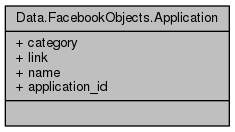
\includegraphics[width=248pt]{class_data_1_1_facebook_objects_1_1_application__coll__graph}
\end{center}
\end{figure}
\subsection*{Properties}
\begin{DoxyCompactItemize}
\item 
string \hyperlink{class_data_1_1_facebook_objects_1_1_application_aa672437a8fd9f3398baf2cd7491a929a}{category}\hspace{0.3cm}{\ttfamily  \mbox{[}get, set\mbox{]}}
\item 
string \hyperlink{class_data_1_1_facebook_objects_1_1_application_ae209b254e59693c4f2ad2c774d908426}{link}\hspace{0.3cm}{\ttfamily  \mbox{[}get, set\mbox{]}}
\item 
string \hyperlink{class_data_1_1_facebook_objects_1_1_application_a792e5e532e207d17755ec6f6a5b7f47f}{name}\hspace{0.3cm}{\ttfamily  \mbox{[}get, set\mbox{]}}
\item 
string \hyperlink{class_data_1_1_facebook_objects_1_1_application_a4033dd840557cd10d936869a4b9dab85}{application\+\_\+id}\hspace{0.3cm}{\ttfamily  \mbox{[}get, set\mbox{]}}
\end{DoxyCompactItemize}


\subsection{Detailed Description}


Definition at line 21 of file Comment.\+cs.



\subsection{Property Documentation}
\index{Data\+::\+Facebook\+Objects\+::\+Application@{Data\+::\+Facebook\+Objects\+::\+Application}!application\+\_\+id@{application\+\_\+id}}
\index{application\+\_\+id@{application\+\_\+id}!Data\+::\+Facebook\+Objects\+::\+Application@{Data\+::\+Facebook\+Objects\+::\+Application}}
\subsubsection[{\texorpdfstring{application\+\_\+id}{application_id}}]{\setlength{\rightskip}{0pt plus 5cm}string Data.\+Facebook\+Objects.\+Application.\+application\+\_\+id\hspace{0.3cm}{\ttfamily [get]}, {\ttfamily [set]}}\hypertarget{class_data_1_1_facebook_objects_1_1_application_a4033dd840557cd10d936869a4b9dab85}{}\label{class_data_1_1_facebook_objects_1_1_application_a4033dd840557cd10d936869a4b9dab85}


Definition at line 26 of file Comment.\+cs.

\index{Data\+::\+Facebook\+Objects\+::\+Application@{Data\+::\+Facebook\+Objects\+::\+Application}!category@{category}}
\index{category@{category}!Data\+::\+Facebook\+Objects\+::\+Application@{Data\+::\+Facebook\+Objects\+::\+Application}}
\subsubsection[{\texorpdfstring{category}{category}}]{\setlength{\rightskip}{0pt plus 5cm}string Data.\+Facebook\+Objects.\+Application.\+category\hspace{0.3cm}{\ttfamily [get]}, {\ttfamily [set]}}\hypertarget{class_data_1_1_facebook_objects_1_1_application_aa672437a8fd9f3398baf2cd7491a929a}{}\label{class_data_1_1_facebook_objects_1_1_application_aa672437a8fd9f3398baf2cd7491a929a}


Definition at line 23 of file Comment.\+cs.



Referenced by Operations.\+Data\+Operations.\+Populate\+N\+E\+T\+Object.\+Populate\+Comments().

\index{Data\+::\+Facebook\+Objects\+::\+Application@{Data\+::\+Facebook\+Objects\+::\+Application}!link@{link}}
\index{link@{link}!Data\+::\+Facebook\+Objects\+::\+Application@{Data\+::\+Facebook\+Objects\+::\+Application}}
\subsubsection[{\texorpdfstring{link}{link}}]{\setlength{\rightskip}{0pt plus 5cm}string Data.\+Facebook\+Objects.\+Application.\+link\hspace{0.3cm}{\ttfamily [get]}, {\ttfamily [set]}}\hypertarget{class_data_1_1_facebook_objects_1_1_application_ae209b254e59693c4f2ad2c774d908426}{}\label{class_data_1_1_facebook_objects_1_1_application_ae209b254e59693c4f2ad2c774d908426}


Definition at line 24 of file Comment.\+cs.

\index{Data\+::\+Facebook\+Objects\+::\+Application@{Data\+::\+Facebook\+Objects\+::\+Application}!name@{name}}
\index{name@{name}!Data\+::\+Facebook\+Objects\+::\+Application@{Data\+::\+Facebook\+Objects\+::\+Application}}
\subsubsection[{\texorpdfstring{name}{name}}]{\setlength{\rightskip}{0pt plus 5cm}string Data.\+Facebook\+Objects.\+Application.\+name\hspace{0.3cm}{\ttfamily [get]}, {\ttfamily [set]}}\hypertarget{class_data_1_1_facebook_objects_1_1_application_a792e5e532e207d17755ec6f6a5b7f47f}{}\label{class_data_1_1_facebook_objects_1_1_application_a792e5e532e207d17755ec6f6a5b7f47f}


Definition at line 25 of file Comment.\+cs.



The documentation for this class was generated from the following file\+:\begin{DoxyCompactItemize}
\item 
Facebook\+Application/\+Data/\+Facebook\+Objects/\hyperlink{_comment_8cs}{Comment.\+cs}\end{DoxyCompactItemize}

\hypertarget{class_operations_1_1_client_operations_1_1_client_get_operations}{}\section{Operations.\+Client\+Operations.\+Client\+Get\+Operations Class Reference}
\label{class_operations_1_1_client_operations_1_1_client_get_operations}\index{Operations.\+Client\+Operations.\+Client\+Get\+Operations@{Operations.\+Client\+Operations.\+Client\+Get\+Operations}}


Inheritance diagram for Operations.\+Client\+Operations.\+Client\+Get\+Operations\+:
\nopagebreak
\begin{figure}[H]
\begin{center}
\leavevmode
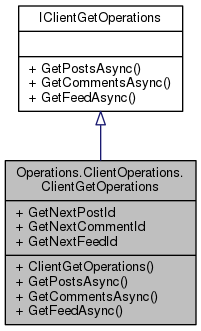
\includegraphics[width=223pt]{class_operations_1_1_client_operations_1_1_client_get_operations__inherit__graph}
\end{center}
\end{figure}


Collaboration diagram for Operations.\+Client\+Operations.\+Client\+Get\+Operations\+:
\nopagebreak
\begin{figure}[H]
\begin{center}
\leavevmode
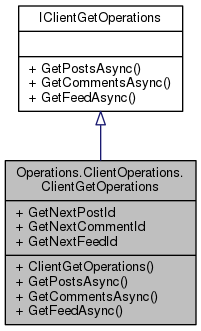
\includegraphics[width=223pt]{class_operations_1_1_client_operations_1_1_client_get_operations__coll__graph}
\end{center}
\end{figure}
\subsection*{Public Member Functions}
\begin{DoxyCompactItemize}
\item 
\hyperlink{class_operations_1_1_client_operations_1_1_client_get_operations_acabd2ed7aa053d1d89c1b9b53f78b337}{Client\+Get\+Operations} (\hyperlink{interface_client_1_1_i_facebook_client}{I\+Facebook\+Client} facebook\+Client)
\begin{DoxyCompactList}\small\item\em Initializes a new instance of the T\+:\+Operations.\+Client\+Operations.\+Client\+Get\+Operations class. \end{DoxyCompactList}\item 
async Task$<$ List$<$ \hyperlink{class_data_1_1_facebook_objects_1_1_post}{Post} $>$ $>$ \hyperlink{class_operations_1_1_client_operations_1_1_client_get_operations_a1f9def392f80708b9a8b3aa2ac84c064}{Get\+Posts\+Async} (string access\+Token, string endpoint, string args)
\begin{DoxyCompactList}\small\item\em Getrequest for posts \end{DoxyCompactList}\item 
async Task$<$ List$<$ \hyperlink{class_data_1_1_facebook_objects_1_1_comment}{Comment} $>$ $>$ \hyperlink{class_operations_1_1_client_operations_1_1_client_get_operations_a6b1649b877d56cac75712b90e0acbeae}{Get\+Comments\+Async} (string access\+Token, string endpoint, string args)
\begin{DoxyCompactList}\small\item\em Getrequest for comments \end{DoxyCompactList}\item 
async Task$<$ List$<$ \hyperlink{class_data_1_1_facebook_objects_1_1_feed}{Feed} $>$ $>$ \hyperlink{class_operations_1_1_client_operations_1_1_client_get_operations_acbb66e0b6496c959a3f33a0c08d096ec}{Get\+Feed\+Async} (string access\+Token, string endpoint, string args)
\begin{DoxyCompactList}\small\item\em Get-\/request for page-\/feed \end{DoxyCompactList}\end{DoxyCompactItemize}
\subsection*{Properties}
\begin{DoxyCompactItemize}
\item 
string \hyperlink{class_operations_1_1_client_operations_1_1_client_get_operations_a19be48989b7a11c85e9c4a1e6e38f26a}{Get\+Next\+Post\+Id}\hspace{0.3cm}{\ttfamily  \mbox{[}get\mbox{]}}
\begin{DoxyCompactList}\small\item\em Gets the get next post identifier. \end{DoxyCompactList}\item 
string \hyperlink{class_operations_1_1_client_operations_1_1_client_get_operations_ad6c8a8843f9039915ee5c47d6ca5536b}{Get\+Next\+Comment\+Id}\hspace{0.3cm}{\ttfamily  \mbox{[}get\mbox{]}}
\begin{DoxyCompactList}\small\item\em Gets the next comment identifier. \end{DoxyCompactList}\item 
string \hyperlink{class_operations_1_1_client_operations_1_1_client_get_operations_aec911a8916000179440a1e4df7dc9ad7}{Get\+Next\+Feed\+Id}\hspace{0.3cm}{\ttfamily  \mbox{[}get\mbox{]}}
\begin{DoxyCompactList}\small\item\em Gets the next feed identifier. \end{DoxyCompactList}\end{DoxyCompactItemize}


\subsection{Detailed Description}


Definition at line 20 of file Client\+Get\+Operation.\+cs.



\subsection{Constructor \& Destructor Documentation}
\index{Operations\+::\+Client\+Operations\+::\+Client\+Get\+Operations@{Operations\+::\+Client\+Operations\+::\+Client\+Get\+Operations}!Client\+Get\+Operations@{Client\+Get\+Operations}}
\index{Client\+Get\+Operations@{Client\+Get\+Operations}!Operations\+::\+Client\+Operations\+::\+Client\+Get\+Operations@{Operations\+::\+Client\+Operations\+::\+Client\+Get\+Operations}}
\subsubsection[{\texorpdfstring{Client\+Get\+Operations(\+I\+Facebook\+Client facebook\+Client)}{ClientGetOperations(IFacebookClient facebookClient)}}]{\setlength{\rightskip}{0pt plus 5cm}Operations.\+Client\+Operations.\+Client\+Get\+Operations.\+Client\+Get\+Operations (
\begin{DoxyParamCaption}
\item[{{\bf I\+Facebook\+Client}}]{facebook\+Client}
\end{DoxyParamCaption}
)}\hypertarget{class_operations_1_1_client_operations_1_1_client_get_operations_acabd2ed7aa053d1d89c1b9b53f78b337}{}\label{class_operations_1_1_client_operations_1_1_client_get_operations_acabd2ed7aa053d1d89c1b9b53f78b337}


Initializes a new instance of the T\+:\+Operations.\+Client\+Operations.\+Client\+Get\+Operations class. 


\begin{DoxyParams}{Parameters}
{\em facebook\+Client} & Facebook client.\\
\hline
\end{DoxyParams}


Definition at line 51 of file Client\+Get\+Operation.\+cs.



\subsection{Member Function Documentation}
\index{Operations\+::\+Client\+Operations\+::\+Client\+Get\+Operations@{Operations\+::\+Client\+Operations\+::\+Client\+Get\+Operations}!Get\+Comments\+Async@{Get\+Comments\+Async}}
\index{Get\+Comments\+Async@{Get\+Comments\+Async}!Operations\+::\+Client\+Operations\+::\+Client\+Get\+Operations@{Operations\+::\+Client\+Operations\+::\+Client\+Get\+Operations}}
\subsubsection[{\texorpdfstring{Get\+Comments\+Async(string access\+Token, string endpoint, string args)}{GetCommentsAsync(string accessToken, string endpoint, string args)}}]{\setlength{\rightskip}{0pt plus 5cm}async Task$<$List$<${\bf Comment}$>$ $>$ Operations.\+Client\+Operations.\+Client\+Get\+Operations.\+Get\+Comments\+Async (
\begin{DoxyParamCaption}
\item[{string}]{access\+Token, }
\item[{string}]{endpoint, }
\item[{string}]{args}
\end{DoxyParamCaption}
)}\hypertarget{class_operations_1_1_client_operations_1_1_client_get_operations_a6b1649b877d56cac75712b90e0acbeae}{}\label{class_operations_1_1_client_operations_1_1_client_get_operations_a6b1649b877d56cac75712b90e0acbeae}


Getrequest for comments 

\begin{DoxyReturn}{Returns}
A list of comment-\/objects/returns$>$ 
\begin{DoxyParams}{Parameters}
{\em access\+Token} & Access token.\\
\hline
{\em endpoint} & Endpoint.\\
\hline
{\em args} & Arguments.\\
\hline
\end{DoxyParams}

\end{DoxyReturn}


Implements \hyperlink{interface_operations_1_1_client_operations_1_1_i_client_get_operations_ae0b222ad5125059baf1201cfeab1abb8}{Operations.\+Client\+Operations.\+I\+Client\+Get\+Operations}.



Definition at line 89 of file Client\+Get\+Operation.\+cs.

\index{Operations\+::\+Client\+Operations\+::\+Client\+Get\+Operations@{Operations\+::\+Client\+Operations\+::\+Client\+Get\+Operations}!Get\+Feed\+Async@{Get\+Feed\+Async}}
\index{Get\+Feed\+Async@{Get\+Feed\+Async}!Operations\+::\+Client\+Operations\+::\+Client\+Get\+Operations@{Operations\+::\+Client\+Operations\+::\+Client\+Get\+Operations}}
\subsubsection[{\texorpdfstring{Get\+Feed\+Async(string access\+Token, string endpoint, string args)}{GetFeedAsync(string accessToken, string endpoint, string args)}}]{\setlength{\rightskip}{0pt plus 5cm}async Task$<$List$<${\bf Feed}$>$ $>$ Operations.\+Client\+Operations.\+Client\+Get\+Operations.\+Get\+Feed\+Async (
\begin{DoxyParamCaption}
\item[{string}]{access\+Token, }
\item[{string}]{endpoint, }
\item[{string}]{args}
\end{DoxyParamCaption}
)}\hypertarget{class_operations_1_1_client_operations_1_1_client_get_operations_acbb66e0b6496c959a3f33a0c08d096ec}{}\label{class_operations_1_1_client_operations_1_1_client_get_operations_acbb66e0b6496c959a3f33a0c08d096ec}


Get-\/request for page-\/feed 

\begin{DoxyReturn}{Returns}
A list of feed-\/objects$>$ 
\end{DoxyReturn}

\begin{DoxyParams}{Parameters}
{\em access\+Token} & Access token.\\
\hline
{\em endpoint} & Endpoint.\\
\hline
{\em args} & Arguments.\\
\hline
\end{DoxyParams}


Implements \hyperlink{interface_operations_1_1_client_operations_1_1_i_client_get_operations_aa4bb87015ba04344e281036d100bf3e7}{Operations.\+Client\+Operations.\+I\+Client\+Get\+Operations}.



Definition at line 115 of file Client\+Get\+Operation.\+cs.

\index{Operations\+::\+Client\+Operations\+::\+Client\+Get\+Operations@{Operations\+::\+Client\+Operations\+::\+Client\+Get\+Operations}!Get\+Posts\+Async@{Get\+Posts\+Async}}
\index{Get\+Posts\+Async@{Get\+Posts\+Async}!Operations\+::\+Client\+Operations\+::\+Client\+Get\+Operations@{Operations\+::\+Client\+Operations\+::\+Client\+Get\+Operations}}
\subsubsection[{\texorpdfstring{Get\+Posts\+Async(string access\+Token, string endpoint, string args)}{GetPostsAsync(string accessToken, string endpoint, string args)}}]{\setlength{\rightskip}{0pt plus 5cm}async Task$<$List$<${\bf Post}$>$ $>$ Operations.\+Client\+Operations.\+Client\+Get\+Operations.\+Get\+Posts\+Async (
\begin{DoxyParamCaption}
\item[{string}]{access\+Token, }
\item[{string}]{endpoint, }
\item[{string}]{args}
\end{DoxyParamCaption}
)}\hypertarget{class_operations_1_1_client_operations_1_1_client_get_operations_a1f9def392f80708b9a8b3aa2ac84c064}{}\label{class_operations_1_1_client_operations_1_1_client_get_operations_a1f9def392f80708b9a8b3aa2ac84c064}


Getrequest for posts 

\begin{DoxyReturn}{Returns}
A list of dynamic post-\/responses
\end{DoxyReturn}

\begin{DoxyParams}{Parameters}
{\em access\+Token} & Access token.\\
\hline
{\em endpoint} & Endpoint.\\
\hline
{\em args} & Arguments.\\
\hline
\end{DoxyParams}


Implements \hyperlink{interface_operations_1_1_client_operations_1_1_i_client_get_operations_ad082c4c82e7cd14d578720d367bb3b3b}{Operations.\+Client\+Operations.\+I\+Client\+Get\+Operations}.



Definition at line 63 of file Client\+Get\+Operation.\+cs.



\subsection{Property Documentation}
\index{Operations\+::\+Client\+Operations\+::\+Client\+Get\+Operations@{Operations\+::\+Client\+Operations\+::\+Client\+Get\+Operations}!Get\+Next\+Comment\+Id@{Get\+Next\+Comment\+Id}}
\index{Get\+Next\+Comment\+Id@{Get\+Next\+Comment\+Id}!Operations\+::\+Client\+Operations\+::\+Client\+Get\+Operations@{Operations\+::\+Client\+Operations\+::\+Client\+Get\+Operations}}
\subsubsection[{\texorpdfstring{Get\+Next\+Comment\+Id}{GetNextCommentId}}]{\setlength{\rightskip}{0pt plus 5cm}string Operations.\+Client\+Operations.\+Client\+Get\+Operations.\+Get\+Next\+Comment\+Id\hspace{0.3cm}{\ttfamily [get]}}\hypertarget{class_operations_1_1_client_operations_1_1_client_get_operations_ad6c8a8843f9039915ee5c47d6ca5536b}{}\label{class_operations_1_1_client_operations_1_1_client_get_operations_ad6c8a8843f9039915ee5c47d6ca5536b}


Gets the next comment identifier. 

The next comment identifier.

Definition at line 149 of file Client\+Get\+Operation.\+cs.

\index{Operations\+::\+Client\+Operations\+::\+Client\+Get\+Operations@{Operations\+::\+Client\+Operations\+::\+Client\+Get\+Operations}!Get\+Next\+Feed\+Id@{Get\+Next\+Feed\+Id}}
\index{Get\+Next\+Feed\+Id@{Get\+Next\+Feed\+Id}!Operations\+::\+Client\+Operations\+::\+Client\+Get\+Operations@{Operations\+::\+Client\+Operations\+::\+Client\+Get\+Operations}}
\subsubsection[{\texorpdfstring{Get\+Next\+Feed\+Id}{GetNextFeedId}}]{\setlength{\rightskip}{0pt plus 5cm}string Operations.\+Client\+Operations.\+Client\+Get\+Operations.\+Get\+Next\+Feed\+Id\hspace{0.3cm}{\ttfamily [get]}}\hypertarget{class_operations_1_1_client_operations_1_1_client_get_operations_aec911a8916000179440a1e4df7dc9ad7}{}\label{class_operations_1_1_client_operations_1_1_client_get_operations_aec911a8916000179440a1e4df7dc9ad7}


Gets the next feed identifier. 

The next feed identifier.

Definition at line 158 of file Client\+Get\+Operation.\+cs.

\index{Operations\+::\+Client\+Operations\+::\+Client\+Get\+Operations@{Operations\+::\+Client\+Operations\+::\+Client\+Get\+Operations}!Get\+Next\+Post\+Id@{Get\+Next\+Post\+Id}}
\index{Get\+Next\+Post\+Id@{Get\+Next\+Post\+Id}!Operations\+::\+Client\+Operations\+::\+Client\+Get\+Operations@{Operations\+::\+Client\+Operations\+::\+Client\+Get\+Operations}}
\subsubsection[{\texorpdfstring{Get\+Next\+Post\+Id}{GetNextPostId}}]{\setlength{\rightskip}{0pt plus 5cm}string Operations.\+Client\+Operations.\+Client\+Get\+Operations.\+Get\+Next\+Post\+Id\hspace{0.3cm}{\ttfamily [get]}}\hypertarget{class_operations_1_1_client_operations_1_1_client_get_operations_a19be48989b7a11c85e9c4a1e6e38f26a}{}\label{class_operations_1_1_client_operations_1_1_client_get_operations_a19be48989b7a11c85e9c4a1e6e38f26a}


Gets the get next post identifier. 

The get next post identifier.

Definition at line 140 of file Client\+Get\+Operation.\+cs.



The documentation for this class was generated from the following file\+:\begin{DoxyCompactItemize}
\item 
Facebook\+Application/\+Operations/\+Client\+Operations/\hyperlink{_client_get_operation_8cs}{Client\+Get\+Operation.\+cs}\end{DoxyCompactItemize}

\hypertarget{class_operations_1_1_client_operations_1_1_client_store_operations}{}\section{Operations.\+Client\+Operations.\+Client\+Store\+Operations Class Reference}
\label{class_operations_1_1_client_operations_1_1_client_store_operations}\index{Operations.\+Client\+Operations.\+Client\+Store\+Operations@{Operations.\+Client\+Operations.\+Client\+Store\+Operations}}


Inheritance diagram for Operations.\+Client\+Operations.\+Client\+Store\+Operations\+:
\nopagebreak
\begin{figure}[H]
\begin{center}
\leavevmode
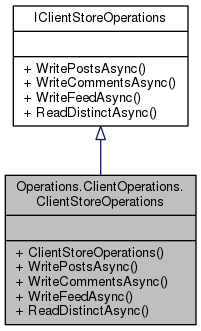
\includegraphics[width=223pt]{class_operations_1_1_client_operations_1_1_client_store_operations__inherit__graph}
\end{center}
\end{figure}


Collaboration diagram for Operations.\+Client\+Operations.\+Client\+Store\+Operations\+:
\nopagebreak
\begin{figure}[H]
\begin{center}
\leavevmode
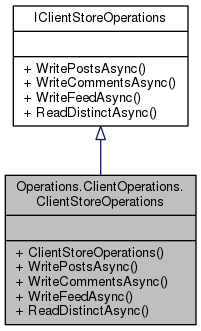
\includegraphics[width=223pt]{class_operations_1_1_client_operations_1_1_client_store_operations__coll__graph}
\end{center}
\end{figure}
\subsection*{Public Member Functions}
\begin{DoxyCompactItemize}
\item 
\hyperlink{class_operations_1_1_client_operations_1_1_client_store_operations_aac158f2176257f4bc25f7cadbd691314}{Client\+Store\+Operations} (\hyperlink{interface_client_1_1_i_d_b_client}{I\+D\+B\+Client} db\+Client)
\begin{DoxyCompactList}\small\item\em Initializes a new instance of the T\+:\+Operations.\+Client\+Operations.\+Client\+Store\+Operations class. \end{DoxyCompactList}\item 
async Task \hyperlink{class_operations_1_1_client_operations_1_1_client_store_operations_aee5d81f7d7dc12cffba2f01ec106bb62}{Write\+Posts\+Async} (I\+Mongo\+Collection$<$ object $>$ collection, List$<$ \hyperlink{class_data_1_1_facebook_objects_1_1_post}{Post} $>$ data)
\begin{DoxyCompactList}\small\item\em Writes chunks of posts to a mongo\+DB collection \end{DoxyCompactList}\item 
async Task \hyperlink{class_operations_1_1_client_operations_1_1_client_store_operations_aafbb730be7ef14c4ee434266a3600f04}{Write\+Comments\+Async} (I\+Mongo\+Collection$<$ object $>$ collection, List$<$ \hyperlink{class_data_1_1_facebook_objects_1_1_comment}{Comment} $>$ data)
\begin{DoxyCompactList}\small\item\em Writes chunks of comments to a mongo\+DB collection \end{DoxyCompactList}\item 
async Task \hyperlink{class_operations_1_1_client_operations_1_1_client_store_operations_a4819e9a632eab5db4e21644512205377}{Write\+Feed\+Async} (I\+Mongo\+Collection$<$ object $>$ collection, List$<$ \hyperlink{class_data_1_1_facebook_objects_1_1_feed}{Feed} $>$ data)
\begin{DoxyCompactList}\small\item\em Writes chunks of feeds to a mongo\+DB collection \end{DoxyCompactList}\item 
async Task$<$ List$<$ object $>$ $>$ \hyperlink{class_operations_1_1_client_operations_1_1_client_store_operations_a998a7bdb46661c725cd8ff2af53c1274}{Read\+Distinct\+Async} (I\+Mongo\+Collection$<$ object $>$ collection, string identifier)
\begin{DoxyCompactList}\small\item\em Reads distinct observations from a mongo\+DB collection \end{DoxyCompactList}\end{DoxyCompactItemize}


\subsection{Detailed Description}


Definition at line 26 of file Client\+Store\+Operations.\+cs.



\subsection{Constructor \& Destructor Documentation}
\index{Operations\+::\+Client\+Operations\+::\+Client\+Store\+Operations@{Operations\+::\+Client\+Operations\+::\+Client\+Store\+Operations}!Client\+Store\+Operations@{Client\+Store\+Operations}}
\index{Client\+Store\+Operations@{Client\+Store\+Operations}!Operations\+::\+Client\+Operations\+::\+Client\+Store\+Operations@{Operations\+::\+Client\+Operations\+::\+Client\+Store\+Operations}}
\subsubsection[{\texorpdfstring{Client\+Store\+Operations(\+I\+D\+B\+Client db\+Client)}{ClientStoreOperations(IDBClient dbClient)}}]{\setlength{\rightskip}{0pt plus 5cm}Operations.\+Client\+Operations.\+Client\+Store\+Operations.\+Client\+Store\+Operations (
\begin{DoxyParamCaption}
\item[{{\bf I\+D\+B\+Client}}]{db\+Client}
\end{DoxyParamCaption}
)}\hypertarget{class_operations_1_1_client_operations_1_1_client_store_operations_aac158f2176257f4bc25f7cadbd691314}{}\label{class_operations_1_1_client_operations_1_1_client_store_operations_aac158f2176257f4bc25f7cadbd691314}


Initializes a new instance of the T\+:\+Operations.\+Client\+Operations.\+Client\+Store\+Operations class. 


\begin{DoxyParams}{Parameters}
{\em db\+Client} & Db client.\\
\hline
\end{DoxyParams}


Definition at line 34 of file Client\+Store\+Operations.\+cs.



\subsection{Member Function Documentation}
\index{Operations\+::\+Client\+Operations\+::\+Client\+Store\+Operations@{Operations\+::\+Client\+Operations\+::\+Client\+Store\+Operations}!Read\+Distinct\+Async@{Read\+Distinct\+Async}}
\index{Read\+Distinct\+Async@{Read\+Distinct\+Async}!Operations\+::\+Client\+Operations\+::\+Client\+Store\+Operations@{Operations\+::\+Client\+Operations\+::\+Client\+Store\+Operations}}
\subsubsection[{\texorpdfstring{Read\+Distinct\+Async(\+I\+Mongo\+Collection$<$ object $>$ collection, string identifier)}{ReadDistinctAsync(IMongoCollection< object > collection, string identifier)}}]{\setlength{\rightskip}{0pt plus 5cm}async Task$<$List$<$object$>$ $>$ Operations.\+Client\+Operations.\+Client\+Store\+Operations.\+Read\+Distinct\+Async (
\begin{DoxyParamCaption}
\item[{I\+Mongo\+Collection$<$ object $>$}]{collection, }
\item[{string}]{identifier}
\end{DoxyParamCaption}
)}\hypertarget{class_operations_1_1_client_operations_1_1_client_store_operations_a998a7bdb46661c725cd8ff2af53c1274}{}\label{class_operations_1_1_client_operations_1_1_client_store_operations_a998a7bdb46661c725cd8ff2af53c1274}


Reads distinct observations from a mongo\+DB collection 

\begin{DoxyReturn}{Returns}
A list of values
\end{DoxyReturn}

\begin{DoxyParams}{Parameters}
{\em collection} & Collection.\\
\hline
{\em identifier} & Any value to search by distinct on.\\
\hline
\end{DoxyParams}


Implements \hyperlink{interface_operations_1_1_client_operations_1_1_i_client_store_operations_af29e0f8002e77e2edf7630bf6c888724}{Operations.\+Client\+Operations.\+I\+Client\+Store\+Operations}.



Definition at line 78 of file Client\+Store\+Operations.\+cs.

\index{Operations\+::\+Client\+Operations\+::\+Client\+Store\+Operations@{Operations\+::\+Client\+Operations\+::\+Client\+Store\+Operations}!Write\+Comments\+Async@{Write\+Comments\+Async}}
\index{Write\+Comments\+Async@{Write\+Comments\+Async}!Operations\+::\+Client\+Operations\+::\+Client\+Store\+Operations@{Operations\+::\+Client\+Operations\+::\+Client\+Store\+Operations}}
\subsubsection[{\texorpdfstring{Write\+Comments\+Async(\+I\+Mongo\+Collection$<$ object $>$ collection, List$<$ Comment $>$ data)}{WriteCommentsAsync(IMongoCollection< object > collection, List< Comment > data)}}]{\setlength{\rightskip}{0pt plus 5cm}async Task Operations.\+Client\+Operations.\+Client\+Store\+Operations.\+Write\+Comments\+Async (
\begin{DoxyParamCaption}
\item[{I\+Mongo\+Collection$<$ object $>$}]{collection, }
\item[{List$<$ {\bf Comment} $>$}]{data}
\end{DoxyParamCaption}
)}\hypertarget{class_operations_1_1_client_operations_1_1_client_store_operations_aafbb730be7ef14c4ee434266a3600f04}{}\label{class_operations_1_1_client_operations_1_1_client_store_operations_aafbb730be7ef14c4ee434266a3600f04}


Writes chunks of comments to a mongo\+DB collection 

\begin{DoxyReturn}{Returns}
Nothing.
\end{DoxyReturn}

\begin{DoxyParams}{Parameters}
{\em collection} & Collection.\\
\hline
{\em data} & \hyperlink{namespace_data}{Data}.\\
\hline
\end{DoxyParams}


Implements \hyperlink{interface_operations_1_1_client_operations_1_1_i_client_store_operations_ac8bf8dadd81dd475a6d5af46f317d5ce}{Operations.\+Client\+Operations.\+I\+Client\+Store\+Operations}.



Definition at line 56 of file Client\+Store\+Operations.\+cs.

\index{Operations\+::\+Client\+Operations\+::\+Client\+Store\+Operations@{Operations\+::\+Client\+Operations\+::\+Client\+Store\+Operations}!Write\+Feed\+Async@{Write\+Feed\+Async}}
\index{Write\+Feed\+Async@{Write\+Feed\+Async}!Operations\+::\+Client\+Operations\+::\+Client\+Store\+Operations@{Operations\+::\+Client\+Operations\+::\+Client\+Store\+Operations}}
\subsubsection[{\texorpdfstring{Write\+Feed\+Async(\+I\+Mongo\+Collection$<$ object $>$ collection, List$<$ Feed $>$ data)}{WriteFeedAsync(IMongoCollection< object > collection, List< Feed > data)}}]{\setlength{\rightskip}{0pt plus 5cm}async Task Operations.\+Client\+Operations.\+Client\+Store\+Operations.\+Write\+Feed\+Async (
\begin{DoxyParamCaption}
\item[{I\+Mongo\+Collection$<$ object $>$}]{collection, }
\item[{List$<$ {\bf Feed} $>$}]{data}
\end{DoxyParamCaption}
)}\hypertarget{class_operations_1_1_client_operations_1_1_client_store_operations_a4819e9a632eab5db4e21644512205377}{}\label{class_operations_1_1_client_operations_1_1_client_store_operations_a4819e9a632eab5db4e21644512205377}


Writes chunks of feeds to a mongo\+DB collection 

\begin{DoxyReturn}{Returns}
Nothing.
\end{DoxyReturn}

\begin{DoxyParams}{Parameters}
{\em collection} & Collection.\\
\hline
{\em data} & \hyperlink{namespace_data}{Data}.\\
\hline
\end{DoxyParams}


Implements \hyperlink{interface_operations_1_1_client_operations_1_1_i_client_store_operations_afba8359dddb9d31552c53591eb0dca7f}{Operations.\+Client\+Operations.\+I\+Client\+Store\+Operations}.



Definition at line 67 of file Client\+Store\+Operations.\+cs.

\index{Operations\+::\+Client\+Operations\+::\+Client\+Store\+Operations@{Operations\+::\+Client\+Operations\+::\+Client\+Store\+Operations}!Write\+Posts\+Async@{Write\+Posts\+Async}}
\index{Write\+Posts\+Async@{Write\+Posts\+Async}!Operations\+::\+Client\+Operations\+::\+Client\+Store\+Operations@{Operations\+::\+Client\+Operations\+::\+Client\+Store\+Operations}}
\subsubsection[{\texorpdfstring{Write\+Posts\+Async(\+I\+Mongo\+Collection$<$ object $>$ collection, List$<$ Post $>$ data)}{WritePostsAsync(IMongoCollection< object > collection, List< Post > data)}}]{\setlength{\rightskip}{0pt plus 5cm}async Task Operations.\+Client\+Operations.\+Client\+Store\+Operations.\+Write\+Posts\+Async (
\begin{DoxyParamCaption}
\item[{I\+Mongo\+Collection$<$ object $>$}]{collection, }
\item[{List$<$ {\bf Post} $>$}]{data}
\end{DoxyParamCaption}
)}\hypertarget{class_operations_1_1_client_operations_1_1_client_store_operations_aee5d81f7d7dc12cffba2f01ec106bb62}{}\label{class_operations_1_1_client_operations_1_1_client_store_operations_aee5d81f7d7dc12cffba2f01ec106bb62}


Writes chunks of posts to a mongo\+DB collection 

\begin{DoxyReturn}{Returns}
Nothing.
\end{DoxyReturn}

\begin{DoxyParams}{Parameters}
{\em collection} & Collection.\\
\hline
{\em data} & \hyperlink{namespace_data}{Data}.\\
\hline
\end{DoxyParams}


Implements \hyperlink{interface_operations_1_1_client_operations_1_1_i_client_store_operations_a2743597c6fcc8febf6f9daf7fa3b9674}{Operations.\+Client\+Operations.\+I\+Client\+Store\+Operations}.



Definition at line 45 of file Client\+Store\+Operations.\+cs.



The documentation for this class was generated from the following file\+:\begin{DoxyCompactItemize}
\item 
Facebook\+Application/\+Operations/\+Client\+Operations/\hyperlink{_client_store_operations_8cs}{Client\+Store\+Operations.\+cs}\end{DoxyCompactItemize}

\hypertarget{class_data_1_1_facebook_objects_1_1_comment}{}\section{Data.\+Facebook\+Objects.\+Comment Class Reference}
\label{class_data_1_1_facebook_objects_1_1_comment}\index{Data.\+Facebook\+Objects.\+Comment@{Data.\+Facebook\+Objects.\+Comment}}


Collaboration diagram for Data.\+Facebook\+Objects.\+Comment\+:
\nopagebreak
\begin{figure}[H]
\begin{center}
\leavevmode
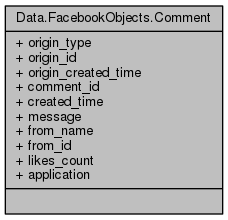
\includegraphics[width=243pt]{class_data_1_1_facebook_objects_1_1_comment__coll__graph}
\end{center}
\end{figure}
\subsection*{Properties}
\begin{DoxyCompactItemize}
\item 
string \hyperlink{class_data_1_1_facebook_objects_1_1_comment_a7dc02ae737535044e97e841357bc40a6}{origin\+\_\+type}\hspace{0.3cm}{\ttfamily  \mbox{[}get, set\mbox{]}}
\item 
string \hyperlink{class_data_1_1_facebook_objects_1_1_comment_aa13d3076050de21b8637566bc1e7b8b1}{origin\+\_\+id}\hspace{0.3cm}{\ttfamily  \mbox{[}get, set\mbox{]}}
\item 
Date\+Time \hyperlink{class_data_1_1_facebook_objects_1_1_comment_a4cd02f87f106d1db97644a8eaf4b2bbb}{origin\+\_\+created\+\_\+time}\hspace{0.3cm}{\ttfamily  \mbox{[}get, set\mbox{]}}
\item 
string \hyperlink{class_data_1_1_facebook_objects_1_1_comment_a4993d3973c20ee4218dbb31d1e265d12}{comment\+\_\+id}\hspace{0.3cm}{\ttfamily  \mbox{[}get, set\mbox{]}}
\item 
Date\+Time \hyperlink{class_data_1_1_facebook_objects_1_1_comment_a3b7f2552fabc98705101aaae56beddd6}{created\+\_\+time}\hspace{0.3cm}{\ttfamily  \mbox{[}get, set\mbox{]}}
\item 
string \hyperlink{class_data_1_1_facebook_objects_1_1_comment_a1fa3625f9aab6c29e764659afffead9c}{message}\hspace{0.3cm}{\ttfamily  \mbox{[}get, set\mbox{]}}
\item 
string \hyperlink{class_data_1_1_facebook_objects_1_1_comment_a07a44e439f904fc5e204c518328d3485}{from\+\_\+name}\hspace{0.3cm}{\ttfamily  \mbox{[}get, set\mbox{]}}
\item 
string \hyperlink{class_data_1_1_facebook_objects_1_1_comment_a05b0fbb7b709d35f6ba260b2df7c523c}{from\+\_\+id}\hspace{0.3cm}{\ttfamily  \mbox{[}get, set\mbox{]}}
\item 
int \hyperlink{class_data_1_1_facebook_objects_1_1_comment_a33cbf2ae949c0d355dec05074c23878f}{likes\+\_\+count}\hspace{0.3cm}{\ttfamily  \mbox{[}get, set\mbox{]}}
\item 
\hyperlink{class_data_1_1_facebook_objects_1_1_application}{Application} \hyperlink{class_data_1_1_facebook_objects_1_1_comment_afcc2f34789206956028283de27326fe7}{application}\hspace{0.3cm}{\ttfamily  \mbox{[}get, set\mbox{]}}
\end{DoxyCompactItemize}


\subsection{Detailed Description}


Definition at line 7 of file Comment.\+cs.



\subsection{Property Documentation}
\index{Data\+::\+Facebook\+Objects\+::\+Comment@{Data\+::\+Facebook\+Objects\+::\+Comment}!application@{application}}
\index{application@{application}!Data\+::\+Facebook\+Objects\+::\+Comment@{Data\+::\+Facebook\+Objects\+::\+Comment}}
\subsubsection[{\texorpdfstring{application}{application}}]{\setlength{\rightskip}{0pt plus 5cm}{\bf Application} Data.\+Facebook\+Objects.\+Comment.\+application\hspace{0.3cm}{\ttfamily [get]}, {\ttfamily [set]}}\hypertarget{class_data_1_1_facebook_objects_1_1_comment_afcc2f34789206956028283de27326fe7}{}\label{class_data_1_1_facebook_objects_1_1_comment_afcc2f34789206956028283de27326fe7}


Definition at line 18 of file Comment.\+cs.

\index{Data\+::\+Facebook\+Objects\+::\+Comment@{Data\+::\+Facebook\+Objects\+::\+Comment}!comment\+\_\+id@{comment\+\_\+id}}
\index{comment\+\_\+id@{comment\+\_\+id}!Data\+::\+Facebook\+Objects\+::\+Comment@{Data\+::\+Facebook\+Objects\+::\+Comment}}
\subsubsection[{\texorpdfstring{comment\+\_\+id}{comment_id}}]{\setlength{\rightskip}{0pt plus 5cm}string Data.\+Facebook\+Objects.\+Comment.\+comment\+\_\+id\hspace{0.3cm}{\ttfamily [get]}, {\ttfamily [set]}}\hypertarget{class_data_1_1_facebook_objects_1_1_comment_a4993d3973c20ee4218dbb31d1e265d12}{}\label{class_data_1_1_facebook_objects_1_1_comment_a4993d3973c20ee4218dbb31d1e265d12}


Definition at line 12 of file Comment.\+cs.

\index{Data\+::\+Facebook\+Objects\+::\+Comment@{Data\+::\+Facebook\+Objects\+::\+Comment}!created\+\_\+time@{created\+\_\+time}}
\index{created\+\_\+time@{created\+\_\+time}!Data\+::\+Facebook\+Objects\+::\+Comment@{Data\+::\+Facebook\+Objects\+::\+Comment}}
\subsubsection[{\texorpdfstring{created\+\_\+time}{created_time}}]{\setlength{\rightskip}{0pt plus 5cm}Date\+Time Data.\+Facebook\+Objects.\+Comment.\+created\+\_\+time\hspace{0.3cm}{\ttfamily [get]}, {\ttfamily [set]}}\hypertarget{class_data_1_1_facebook_objects_1_1_comment_a3b7f2552fabc98705101aaae56beddd6}{}\label{class_data_1_1_facebook_objects_1_1_comment_a3b7f2552fabc98705101aaae56beddd6}


Definition at line 13 of file Comment.\+cs.



Referenced by Operations.\+Data\+Operations.\+Populate\+N\+E\+T\+Object.\+Populate\+Comments().

\index{Data\+::\+Facebook\+Objects\+::\+Comment@{Data\+::\+Facebook\+Objects\+::\+Comment}!from\+\_\+id@{from\+\_\+id}}
\index{from\+\_\+id@{from\+\_\+id}!Data\+::\+Facebook\+Objects\+::\+Comment@{Data\+::\+Facebook\+Objects\+::\+Comment}}
\subsubsection[{\texorpdfstring{from\+\_\+id}{from_id}}]{\setlength{\rightskip}{0pt plus 5cm}string Data.\+Facebook\+Objects.\+Comment.\+from\+\_\+id\hspace{0.3cm}{\ttfamily [get]}, {\ttfamily [set]}}\hypertarget{class_data_1_1_facebook_objects_1_1_comment_a05b0fbb7b709d35f6ba260b2df7c523c}{}\label{class_data_1_1_facebook_objects_1_1_comment_a05b0fbb7b709d35f6ba260b2df7c523c}


Definition at line 16 of file Comment.\+cs.

\index{Data\+::\+Facebook\+Objects\+::\+Comment@{Data\+::\+Facebook\+Objects\+::\+Comment}!from\+\_\+name@{from\+\_\+name}}
\index{from\+\_\+name@{from\+\_\+name}!Data\+::\+Facebook\+Objects\+::\+Comment@{Data\+::\+Facebook\+Objects\+::\+Comment}}
\subsubsection[{\texorpdfstring{from\+\_\+name}{from_name}}]{\setlength{\rightskip}{0pt plus 5cm}string Data.\+Facebook\+Objects.\+Comment.\+from\+\_\+name\hspace{0.3cm}{\ttfamily [get]}, {\ttfamily [set]}}\hypertarget{class_data_1_1_facebook_objects_1_1_comment_a07a44e439f904fc5e204c518328d3485}{}\label{class_data_1_1_facebook_objects_1_1_comment_a07a44e439f904fc5e204c518328d3485}


Definition at line 15 of file Comment.\+cs.

\index{Data\+::\+Facebook\+Objects\+::\+Comment@{Data\+::\+Facebook\+Objects\+::\+Comment}!likes\+\_\+count@{likes\+\_\+count}}
\index{likes\+\_\+count@{likes\+\_\+count}!Data\+::\+Facebook\+Objects\+::\+Comment@{Data\+::\+Facebook\+Objects\+::\+Comment}}
\subsubsection[{\texorpdfstring{likes\+\_\+count}{likes_count}}]{\setlength{\rightskip}{0pt plus 5cm}int Data.\+Facebook\+Objects.\+Comment.\+likes\+\_\+count\hspace{0.3cm}{\ttfamily [get]}, {\ttfamily [set]}}\hypertarget{class_data_1_1_facebook_objects_1_1_comment_a33cbf2ae949c0d355dec05074c23878f}{}\label{class_data_1_1_facebook_objects_1_1_comment_a33cbf2ae949c0d355dec05074c23878f}


Definition at line 17 of file Comment.\+cs.

\index{Data\+::\+Facebook\+Objects\+::\+Comment@{Data\+::\+Facebook\+Objects\+::\+Comment}!message@{message}}
\index{message@{message}!Data\+::\+Facebook\+Objects\+::\+Comment@{Data\+::\+Facebook\+Objects\+::\+Comment}}
\subsubsection[{\texorpdfstring{message}{message}}]{\setlength{\rightskip}{0pt plus 5cm}string Data.\+Facebook\+Objects.\+Comment.\+message\hspace{0.3cm}{\ttfamily [get]}, {\ttfamily [set]}}\hypertarget{class_data_1_1_facebook_objects_1_1_comment_a1fa3625f9aab6c29e764659afffead9c}{}\label{class_data_1_1_facebook_objects_1_1_comment_a1fa3625f9aab6c29e764659afffead9c}


Definition at line 14 of file Comment.\+cs.



Referenced by Operations.\+Data\+Operations.\+Populate\+N\+E\+T\+Object.\+Populate\+Comments().

\index{Data\+::\+Facebook\+Objects\+::\+Comment@{Data\+::\+Facebook\+Objects\+::\+Comment}!origin\+\_\+created\+\_\+time@{origin\+\_\+created\+\_\+time}}
\index{origin\+\_\+created\+\_\+time@{origin\+\_\+created\+\_\+time}!Data\+::\+Facebook\+Objects\+::\+Comment@{Data\+::\+Facebook\+Objects\+::\+Comment}}
\subsubsection[{\texorpdfstring{origin\+\_\+created\+\_\+time}{origin_created_time}}]{\setlength{\rightskip}{0pt plus 5cm}Date\+Time Data.\+Facebook\+Objects.\+Comment.\+origin\+\_\+created\+\_\+time\hspace{0.3cm}{\ttfamily [get]}, {\ttfamily [set]}}\hypertarget{class_data_1_1_facebook_objects_1_1_comment_a4cd02f87f106d1db97644a8eaf4b2bbb}{}\label{class_data_1_1_facebook_objects_1_1_comment_a4cd02f87f106d1db97644a8eaf4b2bbb}


Definition at line 11 of file Comment.\+cs.

\index{Data\+::\+Facebook\+Objects\+::\+Comment@{Data\+::\+Facebook\+Objects\+::\+Comment}!origin\+\_\+id@{origin\+\_\+id}}
\index{origin\+\_\+id@{origin\+\_\+id}!Data\+::\+Facebook\+Objects\+::\+Comment@{Data\+::\+Facebook\+Objects\+::\+Comment}}
\subsubsection[{\texorpdfstring{origin\+\_\+id}{origin_id}}]{\setlength{\rightskip}{0pt plus 5cm}string Data.\+Facebook\+Objects.\+Comment.\+origin\+\_\+id\hspace{0.3cm}{\ttfamily [get]}, {\ttfamily [set]}}\hypertarget{class_data_1_1_facebook_objects_1_1_comment_aa13d3076050de21b8637566bc1e7b8b1}{}\label{class_data_1_1_facebook_objects_1_1_comment_aa13d3076050de21b8637566bc1e7b8b1}


Definition at line 10 of file Comment.\+cs.

\index{Data\+::\+Facebook\+Objects\+::\+Comment@{Data\+::\+Facebook\+Objects\+::\+Comment}!origin\+\_\+type@{origin\+\_\+type}}
\index{origin\+\_\+type@{origin\+\_\+type}!Data\+::\+Facebook\+Objects\+::\+Comment@{Data\+::\+Facebook\+Objects\+::\+Comment}}
\subsubsection[{\texorpdfstring{origin\+\_\+type}{origin_type}}]{\setlength{\rightskip}{0pt plus 5cm}string Data.\+Facebook\+Objects.\+Comment.\+origin\+\_\+type\hspace{0.3cm}{\ttfamily [get]}, {\ttfamily [set]}}\hypertarget{class_data_1_1_facebook_objects_1_1_comment_a7dc02ae737535044e97e841357bc40a6}{}\label{class_data_1_1_facebook_objects_1_1_comment_a7dc02ae737535044e97e841357bc40a6}


Definition at line 9 of file Comment.\+cs.



The documentation for this class was generated from the following file\+:\begin{DoxyCompactItemize}
\item 
Facebook\+Application/\+Data/\+Facebook\+Objects/\hyperlink{_comment_8cs}{Comment.\+cs}\end{DoxyCompactItemize}

\hypertarget{class_client_1_1_d_b_client}{}\section{Client.\+D\+B\+Client Class Reference}
\label{class_client_1_1_d_b_client}\index{Client.\+D\+B\+Client@{Client.\+D\+B\+Client}}


Inheritance diagram for Client.\+D\+B\+Client\+:
\nopagebreak
\begin{figure}[H]
\begin{center}
\leavevmode
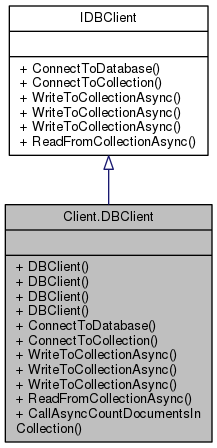
\includegraphics[width=235pt]{class_client_1_1_d_b_client__inherit__graph}
\end{center}
\end{figure}


Collaboration diagram for Client.\+D\+B\+Client\+:
\nopagebreak
\begin{figure}[H]
\begin{center}
\leavevmode
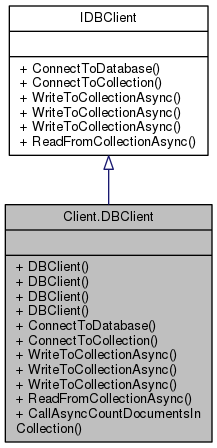
\includegraphics[width=235pt]{class_client_1_1_d_b_client__coll__graph}
\end{center}
\end{figure}
\subsection*{Public Member Functions}
\begin{DoxyCompactItemize}
\item 
\hyperlink{class_client_1_1_d_b_client_a522d138a4a6e287d6e0f4a4e785fc1f6}{D\+B\+Client} ()
\begin{DoxyCompactList}\small\item\em Establishes trivial connection with localhost and returns an instance of a mongodb client \end{DoxyCompactList}\item 
\hyperlink{class_client_1_1_d_b_client_add46a7470fa6c5f9ecf32339428daec5}{D\+B\+Client} (string host, int port)
\begin{DoxyCompactList}\small\item\em Establishes trivial connection with localhost and returns an instance of a mongodb client, with user-\/specified connection parameters. \end{DoxyCompactList}\item 
\hyperlink{class_client_1_1_d_b_client_a2f1223816b5516c8efa71a0ce1f057a7}{D\+B\+Client} (string db, string usr, string pwd)
\begin{DoxyCompactList}\small\item\em Initializes a new instance of the T\+:\+Client.\+D\+B\+Client class. \end{DoxyCompactList}\item 
\hyperlink{class_client_1_1_d_b_client_a69fcdf1545a5cc69b10cba2c5fc51ef2}{D\+B\+Client} (string host, int port, string db, string usr, string pwd)
\begin{DoxyCompactList}\small\item\em Initializes a new instance of the T\+:\+Client.\+D\+B\+Client class. \end{DoxyCompactList}\item 
I\+Mongo\+Database \hyperlink{class_client_1_1_d_b_client_a3e0c25b2cc7d18bc3c5b0ab48f5ce2ea}{Connect\+To\+Database} (string dbname)
\begin{DoxyCompactList}\small\item\em Connects to database. \end{DoxyCompactList}\item 
I\+Mongo\+Collection$<$ object $>$ \hyperlink{class_client_1_1_d_b_client_a527a51d47e38a6290982bb3162e599fe}{Connect\+To\+Collection} (string dbname, string collection)
\begin{DoxyCompactList}\small\item\em Connects to collection. \end{DoxyCompactList}\item 
async Task \hyperlink{class_client_1_1_d_b_client_ae627d0670aa2d71fef0d9fd64c8f9328}{Write\+To\+Collection\+Async} (I\+Mongo\+Collection$<$ object $>$ collection, List$<$ \hyperlink{class_data_1_1_facebook_objects_1_1_post}{Post} $>$ data)
\begin{DoxyCompactList}\small\item\em Asynchronously writes a List of Post-\/objects to a Mongo\+DB collection \end{DoxyCompactList}\item 
async Task \hyperlink{class_client_1_1_d_b_client_a2ad8897568e3885fcd6814366aff1cca}{Write\+To\+Collection\+Async} (I\+Mongo\+Collection$<$ object $>$ collection, List$<$ \hyperlink{class_data_1_1_facebook_objects_1_1_comment}{Comment} $>$ data)
\begin{DoxyCompactList}\small\item\em Asynchronously writes a List of Comment-\/objects to a Mongo\+DB collection \end{DoxyCompactList}\item 
async Task \hyperlink{class_client_1_1_d_b_client_a8ce3c915e127e8b510f6441c50a138e4}{Write\+To\+Collection\+Async} (I\+Mongo\+Collection$<$ object $>$ collection, List$<$ \hyperlink{class_data_1_1_facebook_objects_1_1_feed}{Feed} $>$ data)
\begin{DoxyCompactList}\small\item\em Asynchronously writes a List of Feed-\/objects to a Mongo\+DB collection \end{DoxyCompactList}\item 
async Task \hyperlink{class_client_1_1_d_b_client_aea382fb64f8e3f44fd52fddb841c09a2}{Read\+From\+Collection\+Async} (I\+Mongo\+Collection$<$ object $>$ collection, Filter\+Definition$<$ object $>$ filter=null)
\begin{DoxyCompactList}\small\item\em Reads from collection async. \end{DoxyCompactList}\item 
long \hyperlink{class_client_1_1_d_b_client_a488a378843f1a501333a86dd9d09851e}{Call\+Async\+Count\+Documents\+In\+Collection} (I\+Mongo\+Collection$<$ Bson\+Document $>$ collection)
\begin{DoxyCompactList}\small\item\em Call method to Async\+Count\+Documents\+In\+Collection \end{DoxyCompactList}\end{DoxyCompactItemize}


\subsection{Detailed Description}


Definition at line 29 of file D\+B\+Client.\+cs.



\subsection{Constructor \& Destructor Documentation}
\index{Client\+::\+D\+B\+Client@{Client\+::\+D\+B\+Client}!D\+B\+Client@{D\+B\+Client}}
\index{D\+B\+Client@{D\+B\+Client}!Client\+::\+D\+B\+Client@{Client\+::\+D\+B\+Client}}
\subsubsection[{\texorpdfstring{D\+B\+Client()}{DBClient()}}]{\setlength{\rightskip}{0pt plus 5cm}Client.\+D\+B\+Client.\+D\+B\+Client (
\begin{DoxyParamCaption}
{}
\end{DoxyParamCaption}
)}\hypertarget{class_client_1_1_d_b_client_a522d138a4a6e287d6e0f4a4e785fc1f6}{}\label{class_client_1_1_d_b_client_a522d138a4a6e287d6e0f4a4e785fc1f6}


Establishes trivial connection with localhost and returns an instance of a mongodb client 

\begin{DoxyReturn}{Returns}
A connected instance of a Mongo\+Client
\end{DoxyReturn}


Definition at line 51 of file D\+B\+Client.\+cs.

\index{Client\+::\+D\+B\+Client@{Client\+::\+D\+B\+Client}!D\+B\+Client@{D\+B\+Client}}
\index{D\+B\+Client@{D\+B\+Client}!Client\+::\+D\+B\+Client@{Client\+::\+D\+B\+Client}}
\subsubsection[{\texorpdfstring{D\+B\+Client(string host, int port)}{DBClient(string host, int port)}}]{\setlength{\rightskip}{0pt plus 5cm}Client.\+D\+B\+Client.\+D\+B\+Client (
\begin{DoxyParamCaption}
\item[{string}]{host, }
\item[{int}]{port}
\end{DoxyParamCaption}
)}\hypertarget{class_client_1_1_d_b_client_add46a7470fa6c5f9ecf32339428daec5}{}\label{class_client_1_1_d_b_client_add46a7470fa6c5f9ecf32339428daec5}


Establishes trivial connection with localhost and returns an instance of a mongodb client, with user-\/specified connection parameters. 

\begin{DoxyReturn}{Returns}
A connected instance of a Mongo\+Client
\end{DoxyReturn}

\begin{DoxyParams}{Parameters}
{\em host} & Host to connect to\\
\hline
{\em port} & Port number to connect to\\
\hline
\end{DoxyParams}


Definition at line 67 of file D\+B\+Client.\+cs.

\index{Client\+::\+D\+B\+Client@{Client\+::\+D\+B\+Client}!D\+B\+Client@{D\+B\+Client}}
\index{D\+B\+Client@{D\+B\+Client}!Client\+::\+D\+B\+Client@{Client\+::\+D\+B\+Client}}
\subsubsection[{\texorpdfstring{D\+B\+Client(string db, string usr, string pwd)}{DBClient(string db, string usr, string pwd)}}]{\setlength{\rightskip}{0pt plus 5cm}Client.\+D\+B\+Client.\+D\+B\+Client (
\begin{DoxyParamCaption}
\item[{string}]{db, }
\item[{string}]{usr, }
\item[{string}]{pwd}
\end{DoxyParamCaption}
)}\hypertarget{class_client_1_1_d_b_client_a2f1223816b5516c8efa71a0ce1f057a7}{}\label{class_client_1_1_d_b_client_a2f1223816b5516c8efa71a0ce1f057a7}


Initializes a new instance of the T\+:\+Client.\+D\+B\+Client class. 


\begin{DoxyParams}{Parameters}
{\em db} & Database\\
\hline
{\em usr} & Username\\
\hline
{\em pwd} & Password\\
\hline
\end{DoxyParams}


Definition at line 84 of file D\+B\+Client.\+cs.

\index{Client\+::\+D\+B\+Client@{Client\+::\+D\+B\+Client}!D\+B\+Client@{D\+B\+Client}}
\index{D\+B\+Client@{D\+B\+Client}!Client\+::\+D\+B\+Client@{Client\+::\+D\+B\+Client}}
\subsubsection[{\texorpdfstring{D\+B\+Client(string host, int port, string db, string usr, string pwd)}{DBClient(string host, int port, string db, string usr, string pwd)}}]{\setlength{\rightskip}{0pt plus 5cm}Client.\+D\+B\+Client.\+D\+B\+Client (
\begin{DoxyParamCaption}
\item[{string}]{host, }
\item[{int}]{port, }
\item[{string}]{db, }
\item[{string}]{usr, }
\item[{string}]{pwd}
\end{DoxyParamCaption}
)}\hypertarget{class_client_1_1_d_b_client_a69fcdf1545a5cc69b10cba2c5fc51ef2}{}\label{class_client_1_1_d_b_client_a69fcdf1545a5cc69b10cba2c5fc51ef2}


Initializes a new instance of the T\+:\+Client.\+D\+B\+Client class. 


\begin{DoxyParams}{Parameters}
{\em host} & Host.\\
\hline
{\em port} & Port.\\
\hline
{\em db} & Database\\
\hline
{\em usr} & Username\\
\hline
{\em pwd} & Password\\
\hline
\end{DoxyParams}


Definition at line 103 of file D\+B\+Client.\+cs.



\subsection{Member Function Documentation}
\index{Client\+::\+D\+B\+Client@{Client\+::\+D\+B\+Client}!Call\+Async\+Count\+Documents\+In\+Collection@{Call\+Async\+Count\+Documents\+In\+Collection}}
\index{Call\+Async\+Count\+Documents\+In\+Collection@{Call\+Async\+Count\+Documents\+In\+Collection}!Client\+::\+D\+B\+Client@{Client\+::\+D\+B\+Client}}
\subsubsection[{\texorpdfstring{Call\+Async\+Count\+Documents\+In\+Collection(\+I\+Mongo\+Collection$<$ Bson\+Document $>$ collection)}{CallAsyncCountDocumentsInCollection(IMongoCollection< BsonDocument > collection)}}]{\setlength{\rightskip}{0pt plus 5cm}long Client.\+D\+B\+Client.\+Call\+Async\+Count\+Documents\+In\+Collection (
\begin{DoxyParamCaption}
\item[{I\+Mongo\+Collection$<$ Bson\+Document $>$}]{collection}
\end{DoxyParamCaption}
)}\hypertarget{class_client_1_1_d_b_client_a488a378843f1a501333a86dd9d09851e}{}\label{class_client_1_1_d_b_client_a488a378843f1a501333a86dd9d09851e}


Call method to Async\+Count\+Documents\+In\+Collection 

\begin{DoxyReturn}{Returns}
A numerical value\+: Number of documents
\end{DoxyReturn}

\begin{DoxyParams}{Parameters}
{\em collection} & Collection.\\
\hline
\end{DoxyParams}


Definition at line 230 of file D\+B\+Client.\+cs.

\index{Client\+::\+D\+B\+Client@{Client\+::\+D\+B\+Client}!Connect\+To\+Collection@{Connect\+To\+Collection}}
\index{Connect\+To\+Collection@{Connect\+To\+Collection}!Client\+::\+D\+B\+Client@{Client\+::\+D\+B\+Client}}
\subsubsection[{\texorpdfstring{Connect\+To\+Collection(string dbname, string collection)}{ConnectToCollection(string dbname, string collection)}}]{\setlength{\rightskip}{0pt plus 5cm}I\+Mongo\+Collection$<$object$>$ Client.\+D\+B\+Client.\+Connect\+To\+Collection (
\begin{DoxyParamCaption}
\item[{string}]{dbname, }
\item[{string}]{collection}
\end{DoxyParamCaption}
)}\hypertarget{class_client_1_1_d_b_client_a527a51d47e38a6290982bb3162e599fe}{}\label{class_client_1_1_d_b_client_a527a51d47e38a6290982bb3162e599fe}


Connects to collection. 

\begin{DoxyReturn}{Returns}
A connected instance of a Mongo\+Client.
\end{DoxyReturn}

\begin{DoxyParams}{Parameters}
{\em dbname} & Dbname.\\
\hline
{\em collection} & Collection.\\
\hline
\end{DoxyParams}


Implements \hyperlink{interface_client_1_1_i_d_b_client_a560e1589d25b74448622fcf04949082e}{Client.\+I\+D\+B\+Client}.



Definition at line 130 of file D\+B\+Client.\+cs.



Referenced by Main.\+Program.\+Main().



Here is the caller graph for this function\+:
\nopagebreak
\begin{figure}[H]
\begin{center}
\leavevmode
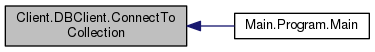
\includegraphics[width=350pt]{class_client_1_1_d_b_client_a527a51d47e38a6290982bb3162e599fe_icgraph}
\end{center}
\end{figure}


\index{Client\+::\+D\+B\+Client@{Client\+::\+D\+B\+Client}!Connect\+To\+Database@{Connect\+To\+Database}}
\index{Connect\+To\+Database@{Connect\+To\+Database}!Client\+::\+D\+B\+Client@{Client\+::\+D\+B\+Client}}
\subsubsection[{\texorpdfstring{Connect\+To\+Database(string dbname)}{ConnectToDatabase(string dbname)}}]{\setlength{\rightskip}{0pt plus 5cm}I\+Mongo\+Database Client.\+D\+B\+Client.\+Connect\+To\+Database (
\begin{DoxyParamCaption}
\item[{string}]{dbname}
\end{DoxyParamCaption}
)}\hypertarget{class_client_1_1_d_b_client_a3e0c25b2cc7d18bc3c5b0ab48f5ce2ea}{}\label{class_client_1_1_d_b_client_a3e0c25b2cc7d18bc3c5b0ab48f5ce2ea}


Connects to database. 

\begin{DoxyReturn}{Returns}
A connected instance of a Mongo\+Client
\end{DoxyReturn}

\begin{DoxyParams}{Parameters}
{\em dbname} & Dbname.\\
\hline
\end{DoxyParams}


Implements \hyperlink{interface_client_1_1_i_d_b_client_a793702523aa275ef01d40f78a96eff01}{Client.\+I\+D\+B\+Client}.



Definition at line 119 of file D\+B\+Client.\+cs.

\index{Client\+::\+D\+B\+Client@{Client\+::\+D\+B\+Client}!Read\+From\+Collection\+Async@{Read\+From\+Collection\+Async}}
\index{Read\+From\+Collection\+Async@{Read\+From\+Collection\+Async}!Client\+::\+D\+B\+Client@{Client\+::\+D\+B\+Client}}
\subsubsection[{\texorpdfstring{Read\+From\+Collection\+Async(\+I\+Mongo\+Collection$<$ object $>$ collection, Filter\+Definition$<$ object $>$ filter=null)}{ReadFromCollectionAsync(IMongoCollection< object > collection, FilterDefinition< object > filter=null)}}]{\setlength{\rightskip}{0pt plus 5cm}async Task Client.\+D\+B\+Client.\+Read\+From\+Collection\+Async (
\begin{DoxyParamCaption}
\item[{I\+Mongo\+Collection$<$ object $>$}]{collection, }
\item[{Filter\+Definition$<$ object $>$}]{filter = {\ttfamily null}}
\end{DoxyParamCaption}
)}\hypertarget{class_client_1_1_d_b_client_aea382fb64f8e3f44fd52fddb841c09a2}{}\label{class_client_1_1_d_b_client_aea382fb64f8e3f44fd52fddb841c09a2}


Reads from collection async. 

\begin{DoxyReturn}{Returns}
The from collection async.
\end{DoxyReturn}

\begin{DoxyParams}{Parameters}
{\em collection} & Collection.\\
\hline
{\em filter} & Filter.\\
\hline
\end{DoxyParams}


Implements \hyperlink{interface_client_1_1_i_d_b_client_ae34d7b6d2b6c624f2dcf537b95aafad1}{Client.\+I\+D\+B\+Client}.



Definition at line 199 of file D\+B\+Client.\+cs.

\index{Client\+::\+D\+B\+Client@{Client\+::\+D\+B\+Client}!Write\+To\+Collection\+Async@{Write\+To\+Collection\+Async}}
\index{Write\+To\+Collection\+Async@{Write\+To\+Collection\+Async}!Client\+::\+D\+B\+Client@{Client\+::\+D\+B\+Client}}
\subsubsection[{\texorpdfstring{Write\+To\+Collection\+Async(\+I\+Mongo\+Collection$<$ object $>$ collection, List$<$ Post $>$ data)}{WriteToCollectionAsync(IMongoCollection< object > collection, List< Post > data)}}]{\setlength{\rightskip}{0pt plus 5cm}async Task Client.\+D\+B\+Client.\+Write\+To\+Collection\+Async (
\begin{DoxyParamCaption}
\item[{I\+Mongo\+Collection$<$ object $>$}]{collection, }
\item[{List$<$ {\bf Post} $>$}]{data}
\end{DoxyParamCaption}
)}\hypertarget{class_client_1_1_d_b_client_ae627d0670aa2d71fef0d9fd64c8f9328}{}\label{class_client_1_1_d_b_client_ae627d0670aa2d71fef0d9fd64c8f9328}


Asynchronously writes a List of Post-\/objects to a Mongo\+DB collection 

\begin{DoxyReturn}{Returns}
The to collection async.
\end{DoxyReturn}

\begin{DoxyParams}{Parameters}
{\em collection} & Collection.\\
\hline
{\em data} & \hyperlink{namespace_data}{Data}.\\
\hline
\end{DoxyParams}


Implements \hyperlink{interface_client_1_1_i_d_b_client_a9fbee0bdce4ec3fc4eb388ba637a855a}{Client.\+I\+D\+B\+Client}.



Definition at line 142 of file D\+B\+Client.\+cs.

\index{Client\+::\+D\+B\+Client@{Client\+::\+D\+B\+Client}!Write\+To\+Collection\+Async@{Write\+To\+Collection\+Async}}
\index{Write\+To\+Collection\+Async@{Write\+To\+Collection\+Async}!Client\+::\+D\+B\+Client@{Client\+::\+D\+B\+Client}}
\subsubsection[{\texorpdfstring{Write\+To\+Collection\+Async(\+I\+Mongo\+Collection$<$ object $>$ collection, List$<$ Comment $>$ data)}{WriteToCollectionAsync(IMongoCollection< object > collection, List< Comment > data)}}]{\setlength{\rightskip}{0pt plus 5cm}async Task Client.\+D\+B\+Client.\+Write\+To\+Collection\+Async (
\begin{DoxyParamCaption}
\item[{I\+Mongo\+Collection$<$ object $>$}]{collection, }
\item[{List$<$ {\bf Comment} $>$}]{data}
\end{DoxyParamCaption}
)}\hypertarget{class_client_1_1_d_b_client_a2ad8897568e3885fcd6814366aff1cca}{}\label{class_client_1_1_d_b_client_a2ad8897568e3885fcd6814366aff1cca}


Asynchronously writes a List of Comment-\/objects to a Mongo\+DB collection 

\begin{DoxyReturn}{Returns}
The to collection async.
\end{DoxyReturn}

\begin{DoxyParams}{Parameters}
{\em collection} & Collection.\\
\hline
{\em data} & \hyperlink{namespace_data}{Data}.\\
\hline
\end{DoxyParams}


Implements \hyperlink{interface_client_1_1_i_d_b_client_af2827db82923cb16cd0295ba89105984}{Client.\+I\+D\+B\+Client}.



Definition at line 161 of file D\+B\+Client.\+cs.

\index{Client\+::\+D\+B\+Client@{Client\+::\+D\+B\+Client}!Write\+To\+Collection\+Async@{Write\+To\+Collection\+Async}}
\index{Write\+To\+Collection\+Async@{Write\+To\+Collection\+Async}!Client\+::\+D\+B\+Client@{Client\+::\+D\+B\+Client}}
\subsubsection[{\texorpdfstring{Write\+To\+Collection\+Async(\+I\+Mongo\+Collection$<$ object $>$ collection, List$<$ Feed $>$ data)}{WriteToCollectionAsync(IMongoCollection< object > collection, List< Feed > data)}}]{\setlength{\rightskip}{0pt plus 5cm}async Task Client.\+D\+B\+Client.\+Write\+To\+Collection\+Async (
\begin{DoxyParamCaption}
\item[{I\+Mongo\+Collection$<$ object $>$}]{collection, }
\item[{List$<$ {\bf Feed} $>$}]{data}
\end{DoxyParamCaption}
)}\hypertarget{class_client_1_1_d_b_client_a8ce3c915e127e8b510f6441c50a138e4}{}\label{class_client_1_1_d_b_client_a8ce3c915e127e8b510f6441c50a138e4}


Asynchronously writes a List of Feed-\/objects to a Mongo\+DB collection 

\begin{DoxyReturn}{Returns}
The to collection async.
\end{DoxyReturn}

\begin{DoxyParams}{Parameters}
{\em collection} & Collection.\\
\hline
{\em data} & \hyperlink{namespace_data}{Data}.\\
\hline
\end{DoxyParams}


Implements \hyperlink{interface_client_1_1_i_d_b_client_ac53ec8495ee3d6afb28196cb9983d2ac}{Client.\+I\+D\+B\+Client}.



Definition at line 180 of file D\+B\+Client.\+cs.



The documentation for this class was generated from the following file\+:\begin{DoxyCompactItemize}
\item 
Facebook\+Application/\+Client/\hyperlink{_d_b_client_8cs}{D\+B\+Client.\+cs}\end{DoxyCompactItemize}

\hypertarget{class_client_1_1_facebook_client}{}\section{Client.\+Facebook\+Client Class Reference}
\label{class_client_1_1_facebook_client}\index{Client.\+Facebook\+Client@{Client.\+Facebook\+Client}}


\hyperlink{class_client_1_1_facebook_client}{Facebook\+Client} Class  




Inheritance diagram for Client.\+Facebook\+Client\+:
\nopagebreak
\begin{figure}[H]
\begin{center}
\leavevmode
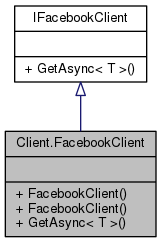
\includegraphics[width=193pt]{class_client_1_1_facebook_client__inherit__graph}
\end{center}
\end{figure}


Collaboration diagram for Client.\+Facebook\+Client\+:
\nopagebreak
\begin{figure}[H]
\begin{center}
\leavevmode
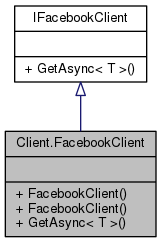
\includegraphics[width=193pt]{class_client_1_1_facebook_client__coll__graph}
\end{center}
\end{figure}
\subsection*{Public Member Functions}
\begin{DoxyCompactItemize}
\item 
\hyperlink{class_client_1_1_facebook_client_a52bc1884b4af1ab80f9b0c780991dc55}{Facebook\+Client} ()
\begin{DoxyCompactList}\small\item\em Initializes a new instance of the T\+:\+Client.\+Facebook\+Client class. \end{DoxyCompactList}\item 
\hyperlink{class_client_1_1_facebook_client_abd40548eb3ac73cbb0755c4ab25fa46f}{Facebook\+Client} (Tuple$<$ string, string $>$ proxy\+Credentials)
\begin{DoxyCompactList}\small\item\em Initializes a new instance of the T\+:\+Client.\+Facebook\+Client class. \end{DoxyCompactList}\item 
async Task$<$ T $>$ \hyperlink{class_client_1_1_facebook_client_aa8feb74481610d6e45da94798656adca}{Get\+Async$<$ T $>$} (string access\+Token, string endpoint, string pageview=null, string args=null)
\begin{DoxyCompactList}\small\item\em Executes \hyperlink{class_client_1_1_facebook_client}{Facebook\+Client} and handles response \end{DoxyCompactList}\end{DoxyCompactItemize}


\subsection{Detailed Description}
\hyperlink{class_client_1_1_facebook_client}{Facebook\+Client} Class 



Definition at line 23 of file Facebook\+Client.\+cs.



\subsection{Constructor \& Destructor Documentation}
\index{Client\+::\+Facebook\+Client@{Client\+::\+Facebook\+Client}!Facebook\+Client@{Facebook\+Client}}
\index{Facebook\+Client@{Facebook\+Client}!Client\+::\+Facebook\+Client@{Client\+::\+Facebook\+Client}}
\subsubsection[{\texorpdfstring{Facebook\+Client()}{FacebookClient()}}]{\setlength{\rightskip}{0pt plus 5cm}Client.\+Facebook\+Client.\+Facebook\+Client (
\begin{DoxyParamCaption}
{}
\end{DoxyParamCaption}
)}\hypertarget{class_client_1_1_facebook_client_a52bc1884b4af1ab80f9b0c780991dc55}{}\label{class_client_1_1_facebook_client_a52bc1884b4af1ab80f9b0c780991dc55}


Initializes a new instance of the T\+:\+Client.\+Facebook\+Client class. 



Definition at line 32 of file Facebook\+Client.\+cs.

\index{Client\+::\+Facebook\+Client@{Client\+::\+Facebook\+Client}!Facebook\+Client@{Facebook\+Client}}
\index{Facebook\+Client@{Facebook\+Client}!Client\+::\+Facebook\+Client@{Client\+::\+Facebook\+Client}}
\subsubsection[{\texorpdfstring{Facebook\+Client(\+Tuple$<$ string, string $>$ proxy\+Credentials)}{FacebookClient(Tuple< string, string > proxyCredentials)}}]{\setlength{\rightskip}{0pt plus 5cm}Client.\+Facebook\+Client.\+Facebook\+Client (
\begin{DoxyParamCaption}
\item[{Tuple$<$ string, string $>$}]{proxy\+Credentials}
\end{DoxyParamCaption}
)}\hypertarget{class_client_1_1_facebook_client_abd40548eb3ac73cbb0755c4ab25fa46f}{}\label{class_client_1_1_facebook_client_abd40548eb3ac73cbb0755c4ab25fa46f}


Initializes a new instance of the T\+:\+Client.\+Facebook\+Client class. 



Definition at line 53 of file Facebook\+Client.\+cs.



\subsection{Member Function Documentation}
\index{Client\+::\+Facebook\+Client@{Client\+::\+Facebook\+Client}!Get\+Async$<$ T $>$@{Get\+Async$<$ T $>$}}
\index{Get\+Async$<$ T $>$@{Get\+Async$<$ T $>$}!Client\+::\+Facebook\+Client@{Client\+::\+Facebook\+Client}}
\subsubsection[{\texorpdfstring{Get\+Async$<$ T $>$(string access\+Token, string endpoint, string pageview=null, string args=null)}{GetAsync< T >(string accessToken, string endpoint, string pageview=null, string args=null)}}]{\setlength{\rightskip}{0pt plus 5cm}async Task$<$T$>$ Client.\+Facebook\+Client.\+Get\+Async$<$ T $>$ (
\begin{DoxyParamCaption}
\item[{string}]{access\+Token, }
\item[{string}]{endpoint, }
\item[{string}]{pageview = {\ttfamily null}, }
\item[{string}]{args = {\ttfamily null}}
\end{DoxyParamCaption}
)}\hypertarget{class_client_1_1_facebook_client_aa8feb74481610d6e45da94798656adca}{}\label{class_client_1_1_facebook_client_aa8feb74481610d6e45da94798656adca}


Executes \hyperlink{class_client_1_1_facebook_client}{Facebook\+Client} and handles response 

\begin{DoxyReturn}{Returns}
The async.
\end{DoxyReturn}

\begin{DoxyParams}{Parameters}
{\em access\+Token} & Access token.\\
\hline
{\em endpoint} & Endpoint.\\
\hline
{\em pageview} & Pageview.\\
\hline
{\em args} & Arguments.\\
\hline
\end{DoxyParams}

\begin{DoxyTemplParams}{Template Parameters}
{\em T} & A \hyperlink{namespace_data}{Data} object class\\
\hline
\end{DoxyTemplParams}


Implements \hyperlink{interface_client_1_1_i_facebook_client_adcc547867f709ce07787df58233c0b85}{Client.\+I\+Facebook\+Client}.



Definition at line 84 of file Facebook\+Client.\+cs.



The documentation for this class was generated from the following file\+:\begin{DoxyCompactItemize}
\item 
Facebook\+Application/\+Client/\hyperlink{_facebook_client_8cs}{Facebook\+Client.\+cs}\end{DoxyCompactItemize}

\hypertarget{class_data_1_1_facebook_objects_1_1_feed}{}\section{Data.\+Facebook\+Objects.\+Feed Class Reference}
\label{class_data_1_1_facebook_objects_1_1_feed}\index{Data.\+Facebook\+Objects.\+Feed@{Data.\+Facebook\+Objects.\+Feed}}


Collaboration diagram for Data.\+Facebook\+Objects.\+Feed\+:
\nopagebreak
\begin{figure}[H]
\begin{center}
\leavevmode
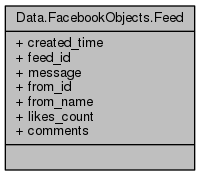
\includegraphics[width=222pt]{class_data_1_1_facebook_objects_1_1_feed__coll__graph}
\end{center}
\end{figure}
\subsection*{Properties}
\begin{DoxyCompactItemize}
\item 
Date\+Time \hyperlink{class_data_1_1_facebook_objects_1_1_feed_afeb5ebd144f9b3990b8ff8d62e552ae2}{created\+\_\+time}\hspace{0.3cm}{\ttfamily  \mbox{[}get, set\mbox{]}}
\item 
string \hyperlink{class_data_1_1_facebook_objects_1_1_feed_acfbbdb5bc789acd45a166c3efc8bcf48}{feed\+\_\+id}\hspace{0.3cm}{\ttfamily  \mbox{[}get, set\mbox{]}}
\item 
string \hyperlink{class_data_1_1_facebook_objects_1_1_feed_a7f3204b98bbca6326617144ed65cd035}{message}\hspace{0.3cm}{\ttfamily  \mbox{[}get, set\mbox{]}}
\item 
string \hyperlink{class_data_1_1_facebook_objects_1_1_feed_afff967ca34c531fc92fd09f359b375c5}{from\+\_\+id}\hspace{0.3cm}{\ttfamily  \mbox{[}get, set\mbox{]}}
\item 
string \hyperlink{class_data_1_1_facebook_objects_1_1_feed_aa50149343a8931ea03ec99fd81f8100c}{from\+\_\+name}\hspace{0.3cm}{\ttfamily  \mbox{[}get, set\mbox{]}}
\item 
int \hyperlink{class_data_1_1_facebook_objects_1_1_feed_aa3afa5771c16a58cc9083d85647dfb18}{likes\+\_\+count}\hspace{0.3cm}{\ttfamily  \mbox{[}get, set\mbox{]}}
\item 
List$<$ \hyperlink{class_data_1_1_facebook_objects_1_1_comment}{Comment} $>$ \hyperlink{class_data_1_1_facebook_objects_1_1_feed_a4af15cfc976d908061796d4df72f1067}{comments}\hspace{0.3cm}{\ttfamily  \mbox{[}get, set\mbox{]}}
\end{DoxyCompactItemize}


\subsection{Detailed Description}


Definition at line 5 of file Feed.\+cs.



\subsection{Property Documentation}
\index{Data\+::\+Facebook\+Objects\+::\+Feed@{Data\+::\+Facebook\+Objects\+::\+Feed}!comments@{comments}}
\index{comments@{comments}!Data\+::\+Facebook\+Objects\+::\+Feed@{Data\+::\+Facebook\+Objects\+::\+Feed}}
\subsubsection[{\texorpdfstring{comments}{comments}}]{\setlength{\rightskip}{0pt plus 5cm}List$<${\bf Comment}$>$ Data.\+Facebook\+Objects.\+Feed.\+comments\hspace{0.3cm}{\ttfamily [get]}, {\ttfamily [set]}}\hypertarget{class_data_1_1_facebook_objects_1_1_feed_a4af15cfc976d908061796d4df72f1067}{}\label{class_data_1_1_facebook_objects_1_1_feed_a4af15cfc976d908061796d4df72f1067}


Definition at line 13 of file Feed.\+cs.

\index{Data\+::\+Facebook\+Objects\+::\+Feed@{Data\+::\+Facebook\+Objects\+::\+Feed}!created\+\_\+time@{created\+\_\+time}}
\index{created\+\_\+time@{created\+\_\+time}!Data\+::\+Facebook\+Objects\+::\+Feed@{Data\+::\+Facebook\+Objects\+::\+Feed}}
\subsubsection[{\texorpdfstring{created\+\_\+time}{created_time}}]{\setlength{\rightskip}{0pt plus 5cm}Date\+Time Data.\+Facebook\+Objects.\+Feed.\+created\+\_\+time\hspace{0.3cm}{\ttfamily [get]}, {\ttfamily [set]}}\hypertarget{class_data_1_1_facebook_objects_1_1_feed_afeb5ebd144f9b3990b8ff8d62e552ae2}{}\label{class_data_1_1_facebook_objects_1_1_feed_afeb5ebd144f9b3990b8ff8d62e552ae2}


Definition at line 7 of file Feed.\+cs.

\index{Data\+::\+Facebook\+Objects\+::\+Feed@{Data\+::\+Facebook\+Objects\+::\+Feed}!feed\+\_\+id@{feed\+\_\+id}}
\index{feed\+\_\+id@{feed\+\_\+id}!Data\+::\+Facebook\+Objects\+::\+Feed@{Data\+::\+Facebook\+Objects\+::\+Feed}}
\subsubsection[{\texorpdfstring{feed\+\_\+id}{feed_id}}]{\setlength{\rightskip}{0pt plus 5cm}string Data.\+Facebook\+Objects.\+Feed.\+feed\+\_\+id\hspace{0.3cm}{\ttfamily [get]}, {\ttfamily [set]}}\hypertarget{class_data_1_1_facebook_objects_1_1_feed_acfbbdb5bc789acd45a166c3efc8bcf48}{}\label{class_data_1_1_facebook_objects_1_1_feed_acfbbdb5bc789acd45a166c3efc8bcf48}


Definition at line 8 of file Feed.\+cs.

\index{Data\+::\+Facebook\+Objects\+::\+Feed@{Data\+::\+Facebook\+Objects\+::\+Feed}!from\+\_\+id@{from\+\_\+id}}
\index{from\+\_\+id@{from\+\_\+id}!Data\+::\+Facebook\+Objects\+::\+Feed@{Data\+::\+Facebook\+Objects\+::\+Feed}}
\subsubsection[{\texorpdfstring{from\+\_\+id}{from_id}}]{\setlength{\rightskip}{0pt plus 5cm}string Data.\+Facebook\+Objects.\+Feed.\+from\+\_\+id\hspace{0.3cm}{\ttfamily [get]}, {\ttfamily [set]}}\hypertarget{class_data_1_1_facebook_objects_1_1_feed_afff967ca34c531fc92fd09f359b375c5}{}\label{class_data_1_1_facebook_objects_1_1_feed_afff967ca34c531fc92fd09f359b375c5}


Definition at line 10 of file Feed.\+cs.

\index{Data\+::\+Facebook\+Objects\+::\+Feed@{Data\+::\+Facebook\+Objects\+::\+Feed}!from\+\_\+name@{from\+\_\+name}}
\index{from\+\_\+name@{from\+\_\+name}!Data\+::\+Facebook\+Objects\+::\+Feed@{Data\+::\+Facebook\+Objects\+::\+Feed}}
\subsubsection[{\texorpdfstring{from\+\_\+name}{from_name}}]{\setlength{\rightskip}{0pt plus 5cm}string Data.\+Facebook\+Objects.\+Feed.\+from\+\_\+name\hspace{0.3cm}{\ttfamily [get]}, {\ttfamily [set]}}\hypertarget{class_data_1_1_facebook_objects_1_1_feed_aa50149343a8931ea03ec99fd81f8100c}{}\label{class_data_1_1_facebook_objects_1_1_feed_aa50149343a8931ea03ec99fd81f8100c}


Definition at line 11 of file Feed.\+cs.

\index{Data\+::\+Facebook\+Objects\+::\+Feed@{Data\+::\+Facebook\+Objects\+::\+Feed}!likes\+\_\+count@{likes\+\_\+count}}
\index{likes\+\_\+count@{likes\+\_\+count}!Data\+::\+Facebook\+Objects\+::\+Feed@{Data\+::\+Facebook\+Objects\+::\+Feed}}
\subsubsection[{\texorpdfstring{likes\+\_\+count}{likes_count}}]{\setlength{\rightskip}{0pt plus 5cm}int Data.\+Facebook\+Objects.\+Feed.\+likes\+\_\+count\hspace{0.3cm}{\ttfamily [get]}, {\ttfamily [set]}}\hypertarget{class_data_1_1_facebook_objects_1_1_feed_aa3afa5771c16a58cc9083d85647dfb18}{}\label{class_data_1_1_facebook_objects_1_1_feed_aa3afa5771c16a58cc9083d85647dfb18}


Definition at line 12 of file Feed.\+cs.

\index{Data\+::\+Facebook\+Objects\+::\+Feed@{Data\+::\+Facebook\+Objects\+::\+Feed}!message@{message}}
\index{message@{message}!Data\+::\+Facebook\+Objects\+::\+Feed@{Data\+::\+Facebook\+Objects\+::\+Feed}}
\subsubsection[{\texorpdfstring{message}{message}}]{\setlength{\rightskip}{0pt plus 5cm}string Data.\+Facebook\+Objects.\+Feed.\+message\hspace{0.3cm}{\ttfamily [get]}, {\ttfamily [set]}}\hypertarget{class_data_1_1_facebook_objects_1_1_feed_a7f3204b98bbca6326617144ed65cd035}{}\label{class_data_1_1_facebook_objects_1_1_feed_a7f3204b98bbca6326617144ed65cd035}


Definition at line 9 of file Feed.\+cs.



Referenced by Operations.\+Data\+Operations.\+Populate\+N\+E\+T\+Object.\+Populate\+Feed().



The documentation for this class was generated from the following file\+:\begin{DoxyCompactItemize}
\item 
Facebook\+Application/\+Data/\+Facebook\+Objects/\hyperlink{_feed_8cs}{Feed.\+cs}\end{DoxyCompactItemize}

\hypertarget{interface_operations_1_1_client_operations_1_1_i_client_get_operations}{}\section{Operations.\+Client\+Operations.\+I\+Client\+Get\+Operations Interface Reference}
\label{interface_operations_1_1_client_operations_1_1_i_client_get_operations}\index{Operations.\+Client\+Operations.\+I\+Client\+Get\+Operations@{Operations.\+Client\+Operations.\+I\+Client\+Get\+Operations}}


Inheritance diagram for Operations.\+Client\+Operations.\+I\+Client\+Get\+Operations\+:
\nopagebreak
\begin{figure}[H]
\begin{center}
\leavevmode
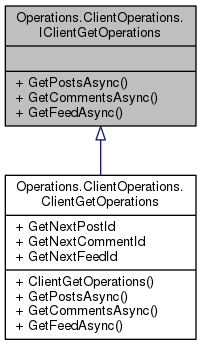
\includegraphics[width=223pt]{interface_operations_1_1_client_operations_1_1_i_client_get_operations__inherit__graph}
\end{center}
\end{figure}


Collaboration diagram for Operations.\+Client\+Operations.\+I\+Client\+Get\+Operations\+:
\nopagebreak
\begin{figure}[H]
\begin{center}
\leavevmode
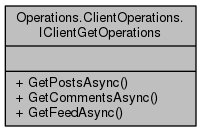
\includegraphics[width=223pt]{interface_operations_1_1_client_operations_1_1_i_client_get_operations__coll__graph}
\end{center}
\end{figure}
\subsection*{Public Member Functions}
\begin{DoxyCompactItemize}
\item 
Task$<$ List$<$ \hyperlink{class_data_1_1_facebook_objects_1_1_post}{Post} $>$ $>$ \hyperlink{interface_operations_1_1_client_operations_1_1_i_client_get_operations_ad082c4c82e7cd14d578720d367bb3b3b}{Get\+Posts\+Async} (string acces\+Token, string pageview, string args)
\item 
Task$<$ List$<$ \hyperlink{class_data_1_1_facebook_objects_1_1_comment}{Comment} $>$ $>$ \hyperlink{interface_operations_1_1_client_operations_1_1_i_client_get_operations_ae0b222ad5125059baf1201cfeab1abb8}{Get\+Comments\+Async} (string access\+Token, string endpoint, string args)
\item 
Task$<$ List$<$ \hyperlink{class_data_1_1_facebook_objects_1_1_feed}{Feed} $>$ $>$ \hyperlink{interface_operations_1_1_client_operations_1_1_i_client_get_operations_aa4bb87015ba04344e281036d100bf3e7}{Get\+Feed\+Async} (string access\+Token, string endpoint, string args)
\end{DoxyCompactItemize}


\subsection{Detailed Description}


Definition at line 13 of file Client\+Get\+Operation.\+cs.



\subsection{Member Function Documentation}
\index{Operations\+::\+Client\+Operations\+::\+I\+Client\+Get\+Operations@{Operations\+::\+Client\+Operations\+::\+I\+Client\+Get\+Operations}!Get\+Comments\+Async@{Get\+Comments\+Async}}
\index{Get\+Comments\+Async@{Get\+Comments\+Async}!Operations\+::\+Client\+Operations\+::\+I\+Client\+Get\+Operations@{Operations\+::\+Client\+Operations\+::\+I\+Client\+Get\+Operations}}
\subsubsection[{\texorpdfstring{Get\+Comments\+Async(string access\+Token, string endpoint, string args)}{GetCommentsAsync(string accessToken, string endpoint, string args)}}]{\setlength{\rightskip}{0pt plus 5cm}Task$<$List$<${\bf Comment}$>$ $>$ Operations.\+Client\+Operations.\+I\+Client\+Get\+Operations.\+Get\+Comments\+Async (
\begin{DoxyParamCaption}
\item[{string}]{access\+Token, }
\item[{string}]{endpoint, }
\item[{string}]{args}
\end{DoxyParamCaption}
)}\hypertarget{interface_operations_1_1_client_operations_1_1_i_client_get_operations_ae0b222ad5125059baf1201cfeab1abb8}{}\label{interface_operations_1_1_client_operations_1_1_i_client_get_operations_ae0b222ad5125059baf1201cfeab1abb8}


Implemented in \hyperlink{class_operations_1_1_client_operations_1_1_client_get_operations_a6b1649b877d56cac75712b90e0acbeae}{Operations.\+Client\+Operations.\+Client\+Get\+Operations}.

\index{Operations\+::\+Client\+Operations\+::\+I\+Client\+Get\+Operations@{Operations\+::\+Client\+Operations\+::\+I\+Client\+Get\+Operations}!Get\+Feed\+Async@{Get\+Feed\+Async}}
\index{Get\+Feed\+Async@{Get\+Feed\+Async}!Operations\+::\+Client\+Operations\+::\+I\+Client\+Get\+Operations@{Operations\+::\+Client\+Operations\+::\+I\+Client\+Get\+Operations}}
\subsubsection[{\texorpdfstring{Get\+Feed\+Async(string access\+Token, string endpoint, string args)}{GetFeedAsync(string accessToken, string endpoint, string args)}}]{\setlength{\rightskip}{0pt plus 5cm}Task$<$List$<${\bf Feed}$>$ $>$ Operations.\+Client\+Operations.\+I\+Client\+Get\+Operations.\+Get\+Feed\+Async (
\begin{DoxyParamCaption}
\item[{string}]{access\+Token, }
\item[{string}]{endpoint, }
\item[{string}]{args}
\end{DoxyParamCaption}
)}\hypertarget{interface_operations_1_1_client_operations_1_1_i_client_get_operations_aa4bb87015ba04344e281036d100bf3e7}{}\label{interface_operations_1_1_client_operations_1_1_i_client_get_operations_aa4bb87015ba04344e281036d100bf3e7}


Implemented in \hyperlink{class_operations_1_1_client_operations_1_1_client_get_operations_acbb66e0b6496c959a3f33a0c08d096ec}{Operations.\+Client\+Operations.\+Client\+Get\+Operations}.

\index{Operations\+::\+Client\+Operations\+::\+I\+Client\+Get\+Operations@{Operations\+::\+Client\+Operations\+::\+I\+Client\+Get\+Operations}!Get\+Posts\+Async@{Get\+Posts\+Async}}
\index{Get\+Posts\+Async@{Get\+Posts\+Async}!Operations\+::\+Client\+Operations\+::\+I\+Client\+Get\+Operations@{Operations\+::\+Client\+Operations\+::\+I\+Client\+Get\+Operations}}
\subsubsection[{\texorpdfstring{Get\+Posts\+Async(string acces\+Token, string pageview, string args)}{GetPostsAsync(string accesToken, string pageview, string args)}}]{\setlength{\rightskip}{0pt plus 5cm}Task$<$List$<${\bf Post}$>$ $>$ Operations.\+Client\+Operations.\+I\+Client\+Get\+Operations.\+Get\+Posts\+Async (
\begin{DoxyParamCaption}
\item[{string}]{acces\+Token, }
\item[{string}]{pageview, }
\item[{string}]{args}
\end{DoxyParamCaption}
)}\hypertarget{interface_operations_1_1_client_operations_1_1_i_client_get_operations_ad082c4c82e7cd14d578720d367bb3b3b}{}\label{interface_operations_1_1_client_operations_1_1_i_client_get_operations_ad082c4c82e7cd14d578720d367bb3b3b}


Implemented in \hyperlink{class_operations_1_1_client_operations_1_1_client_get_operations_a1f9def392f80708b9a8b3aa2ac84c064}{Operations.\+Client\+Operations.\+Client\+Get\+Operations}.



The documentation for this interface was generated from the following file\+:\begin{DoxyCompactItemize}
\item 
Facebook\+Application/\+Operations/\+Client\+Operations/\hyperlink{_client_get_operation_8cs}{Client\+Get\+Operation.\+cs}\end{DoxyCompactItemize}

\hypertarget{interface_operations_1_1_client_operations_1_1_i_client_store_operations}{}\section{Operations.\+Client\+Operations.\+I\+Client\+Store\+Operations Interface Reference}
\label{interface_operations_1_1_client_operations_1_1_i_client_store_operations}\index{Operations.\+Client\+Operations.\+I\+Client\+Store\+Operations@{Operations.\+Client\+Operations.\+I\+Client\+Store\+Operations}}


Inheritance diagram for Operations.\+Client\+Operations.\+I\+Client\+Store\+Operations\+:
\nopagebreak
\begin{figure}[H]
\begin{center}
\leavevmode
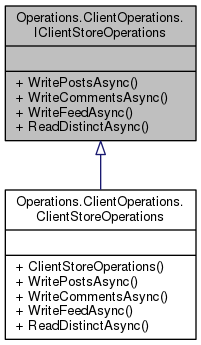
\includegraphics[width=223pt]{interface_operations_1_1_client_operations_1_1_i_client_store_operations__inherit__graph}
\end{center}
\end{figure}


Collaboration diagram for Operations.\+Client\+Operations.\+I\+Client\+Store\+Operations\+:
\nopagebreak
\begin{figure}[H]
\begin{center}
\leavevmode
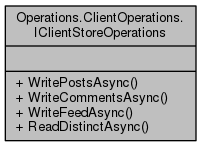
\includegraphics[width=223pt]{interface_operations_1_1_client_operations_1_1_i_client_store_operations__coll__graph}
\end{center}
\end{figure}
\subsection*{Public Member Functions}
\begin{DoxyCompactItemize}
\item 
Task \hyperlink{interface_operations_1_1_client_operations_1_1_i_client_store_operations_a2743597c6fcc8febf6f9daf7fa3b9674}{Write\+Posts\+Async} (I\+Mongo\+Collection$<$ object $>$ collection, List$<$ \hyperlink{class_data_1_1_facebook_objects_1_1_post}{Post} $>$ data)
\item 
Task \hyperlink{interface_operations_1_1_client_operations_1_1_i_client_store_operations_ac8bf8dadd81dd475a6d5af46f317d5ce}{Write\+Comments\+Async} (I\+Mongo\+Collection$<$ object $>$ collection, List$<$ \hyperlink{class_data_1_1_facebook_objects_1_1_comment}{Comment} $>$ data)
\item 
Task \hyperlink{interface_operations_1_1_client_operations_1_1_i_client_store_operations_afba8359dddb9d31552c53591eb0dca7f}{Write\+Feed\+Async} (I\+Mongo\+Collection$<$ object $>$ collection, List$<$ \hyperlink{class_data_1_1_facebook_objects_1_1_feed}{Feed} $>$ data)
\item 
Task$<$ List$<$ object $>$ $>$ \hyperlink{interface_operations_1_1_client_operations_1_1_i_client_store_operations_af29e0f8002e77e2edf7630bf6c888724}{Read\+Distinct\+Async} (I\+Mongo\+Collection$<$ object $>$ collection, string identifier)
\end{DoxyCompactItemize}


\subsection{Detailed Description}


Definition at line 18 of file Client\+Store\+Operations.\+cs.



\subsection{Member Function Documentation}
\index{Operations\+::\+Client\+Operations\+::\+I\+Client\+Store\+Operations@{Operations\+::\+Client\+Operations\+::\+I\+Client\+Store\+Operations}!Read\+Distinct\+Async@{Read\+Distinct\+Async}}
\index{Read\+Distinct\+Async@{Read\+Distinct\+Async}!Operations\+::\+Client\+Operations\+::\+I\+Client\+Store\+Operations@{Operations\+::\+Client\+Operations\+::\+I\+Client\+Store\+Operations}}
\subsubsection[{\texorpdfstring{Read\+Distinct\+Async(\+I\+Mongo\+Collection$<$ object $>$ collection, string identifier)}{ReadDistinctAsync(IMongoCollection< object > collection, string identifier)}}]{\setlength{\rightskip}{0pt plus 5cm}Task$<$List$<$object$>$ $>$ Operations.\+Client\+Operations.\+I\+Client\+Store\+Operations.\+Read\+Distinct\+Async (
\begin{DoxyParamCaption}
\item[{I\+Mongo\+Collection$<$ object $>$}]{collection, }
\item[{string}]{identifier}
\end{DoxyParamCaption}
)}\hypertarget{interface_operations_1_1_client_operations_1_1_i_client_store_operations_af29e0f8002e77e2edf7630bf6c888724}{}\label{interface_operations_1_1_client_operations_1_1_i_client_store_operations_af29e0f8002e77e2edf7630bf6c888724}


Implemented in \hyperlink{class_operations_1_1_client_operations_1_1_client_store_operations_a998a7bdb46661c725cd8ff2af53c1274}{Operations.\+Client\+Operations.\+Client\+Store\+Operations}.

\index{Operations\+::\+Client\+Operations\+::\+I\+Client\+Store\+Operations@{Operations\+::\+Client\+Operations\+::\+I\+Client\+Store\+Operations}!Write\+Comments\+Async@{Write\+Comments\+Async}}
\index{Write\+Comments\+Async@{Write\+Comments\+Async}!Operations\+::\+Client\+Operations\+::\+I\+Client\+Store\+Operations@{Operations\+::\+Client\+Operations\+::\+I\+Client\+Store\+Operations}}
\subsubsection[{\texorpdfstring{Write\+Comments\+Async(\+I\+Mongo\+Collection$<$ object $>$ collection, List$<$ Comment $>$ data)}{WriteCommentsAsync(IMongoCollection< object > collection, List< Comment > data)}}]{\setlength{\rightskip}{0pt plus 5cm}Task Operations.\+Client\+Operations.\+I\+Client\+Store\+Operations.\+Write\+Comments\+Async (
\begin{DoxyParamCaption}
\item[{I\+Mongo\+Collection$<$ object $>$}]{collection, }
\item[{List$<$ {\bf Comment} $>$}]{data}
\end{DoxyParamCaption}
)}\hypertarget{interface_operations_1_1_client_operations_1_1_i_client_store_operations_ac8bf8dadd81dd475a6d5af46f317d5ce}{}\label{interface_operations_1_1_client_operations_1_1_i_client_store_operations_ac8bf8dadd81dd475a6d5af46f317d5ce}


Implemented in \hyperlink{class_operations_1_1_client_operations_1_1_client_store_operations_aafbb730be7ef14c4ee434266a3600f04}{Operations.\+Client\+Operations.\+Client\+Store\+Operations}.

\index{Operations\+::\+Client\+Operations\+::\+I\+Client\+Store\+Operations@{Operations\+::\+Client\+Operations\+::\+I\+Client\+Store\+Operations}!Write\+Feed\+Async@{Write\+Feed\+Async}}
\index{Write\+Feed\+Async@{Write\+Feed\+Async}!Operations\+::\+Client\+Operations\+::\+I\+Client\+Store\+Operations@{Operations\+::\+Client\+Operations\+::\+I\+Client\+Store\+Operations}}
\subsubsection[{\texorpdfstring{Write\+Feed\+Async(\+I\+Mongo\+Collection$<$ object $>$ collection, List$<$ Feed $>$ data)}{WriteFeedAsync(IMongoCollection< object > collection, List< Feed > data)}}]{\setlength{\rightskip}{0pt plus 5cm}Task Operations.\+Client\+Operations.\+I\+Client\+Store\+Operations.\+Write\+Feed\+Async (
\begin{DoxyParamCaption}
\item[{I\+Mongo\+Collection$<$ object $>$}]{collection, }
\item[{List$<$ {\bf Feed} $>$}]{data}
\end{DoxyParamCaption}
)}\hypertarget{interface_operations_1_1_client_operations_1_1_i_client_store_operations_afba8359dddb9d31552c53591eb0dca7f}{}\label{interface_operations_1_1_client_operations_1_1_i_client_store_operations_afba8359dddb9d31552c53591eb0dca7f}


Implemented in \hyperlink{class_operations_1_1_client_operations_1_1_client_store_operations_a4819e9a632eab5db4e21644512205377}{Operations.\+Client\+Operations.\+Client\+Store\+Operations}.

\index{Operations\+::\+Client\+Operations\+::\+I\+Client\+Store\+Operations@{Operations\+::\+Client\+Operations\+::\+I\+Client\+Store\+Operations}!Write\+Posts\+Async@{Write\+Posts\+Async}}
\index{Write\+Posts\+Async@{Write\+Posts\+Async}!Operations\+::\+Client\+Operations\+::\+I\+Client\+Store\+Operations@{Operations\+::\+Client\+Operations\+::\+I\+Client\+Store\+Operations}}
\subsubsection[{\texorpdfstring{Write\+Posts\+Async(\+I\+Mongo\+Collection$<$ object $>$ collection, List$<$ Post $>$ data)}{WritePostsAsync(IMongoCollection< object > collection, List< Post > data)}}]{\setlength{\rightskip}{0pt plus 5cm}Task Operations.\+Client\+Operations.\+I\+Client\+Store\+Operations.\+Write\+Posts\+Async (
\begin{DoxyParamCaption}
\item[{I\+Mongo\+Collection$<$ object $>$}]{collection, }
\item[{List$<$ {\bf Post} $>$}]{data}
\end{DoxyParamCaption}
)}\hypertarget{interface_operations_1_1_client_operations_1_1_i_client_store_operations_a2743597c6fcc8febf6f9daf7fa3b9674}{}\label{interface_operations_1_1_client_operations_1_1_i_client_store_operations_a2743597c6fcc8febf6f9daf7fa3b9674}


Implemented in \hyperlink{class_operations_1_1_client_operations_1_1_client_store_operations_aee5d81f7d7dc12cffba2f01ec106bb62}{Operations.\+Client\+Operations.\+Client\+Store\+Operations}.



The documentation for this interface was generated from the following file\+:\begin{DoxyCompactItemize}
\item 
Facebook\+Application/\+Operations/\+Client\+Operations/\hyperlink{_client_store_operations_8cs}{Client\+Store\+Operations.\+cs}\end{DoxyCompactItemize}

\hypertarget{interface_client_1_1_i_d_b_client}{}\section{Client.\+I\+D\+B\+Client Interface Reference}
\label{interface_client_1_1_i_d_b_client}\index{Client.\+I\+D\+B\+Client@{Client.\+I\+D\+B\+Client}}


Inheritance diagram for Client.\+I\+D\+B\+Client\+:
\nopagebreak
\begin{figure}[H]
\begin{center}
\leavevmode
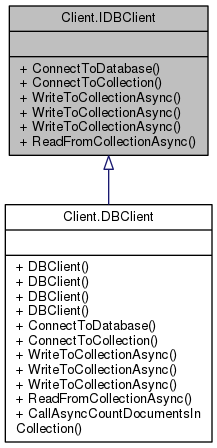
\includegraphics[width=235pt]{interface_client_1_1_i_d_b_client__inherit__graph}
\end{center}
\end{figure}


Collaboration diagram for Client.\+I\+D\+B\+Client\+:
\nopagebreak
\begin{figure}[H]
\begin{center}
\leavevmode
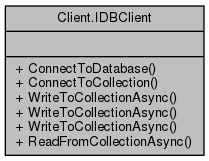
\includegraphics[width=229pt]{interface_client_1_1_i_d_b_client__coll__graph}
\end{center}
\end{figure}
\subsection*{Public Member Functions}
\begin{DoxyCompactItemize}
\item 
I\+Mongo\+Database \hyperlink{interface_client_1_1_i_d_b_client_a793702523aa275ef01d40f78a96eff01}{Connect\+To\+Database} (string dbname)
\item 
I\+Mongo\+Collection$<$ object $>$ \hyperlink{interface_client_1_1_i_d_b_client_a560e1589d25b74448622fcf04949082e}{Connect\+To\+Collection} (string dbname, string collection)
\item 
Task \hyperlink{interface_client_1_1_i_d_b_client_a9fbee0bdce4ec3fc4eb388ba637a855a}{Write\+To\+Collection\+Async} (I\+Mongo\+Collection$<$ object $>$ collection, List$<$ \hyperlink{class_data_1_1_facebook_objects_1_1_post}{Post} $>$ data)
\item 
Task \hyperlink{interface_client_1_1_i_d_b_client_af2827db82923cb16cd0295ba89105984}{Write\+To\+Collection\+Async} (I\+Mongo\+Collection$<$ object $>$ collection, List$<$ \hyperlink{class_data_1_1_facebook_objects_1_1_comment}{Comment} $>$ data)
\item 
Task \hyperlink{interface_client_1_1_i_d_b_client_ac53ec8495ee3d6afb28196cb9983d2ac}{Write\+To\+Collection\+Async} (I\+Mongo\+Collection$<$ object $>$ collection, List$<$ \hyperlink{class_data_1_1_facebook_objects_1_1_feed}{Feed} $>$ data)
\item 
Task \hyperlink{interface_client_1_1_i_d_b_client_ae34d7b6d2b6c624f2dcf537b95aafad1}{Read\+From\+Collection\+Async} (I\+Mongo\+Collection$<$ object $>$ collection, Filter\+Definition$<$ object $>$ filter=null)
\end{DoxyCompactItemize}


\subsection{Detailed Description}


Definition at line 14 of file D\+B\+Client.\+cs.



\subsection{Member Function Documentation}
\index{Client\+::\+I\+D\+B\+Client@{Client\+::\+I\+D\+B\+Client}!Connect\+To\+Collection@{Connect\+To\+Collection}}
\index{Connect\+To\+Collection@{Connect\+To\+Collection}!Client\+::\+I\+D\+B\+Client@{Client\+::\+I\+D\+B\+Client}}
\subsubsection[{\texorpdfstring{Connect\+To\+Collection(string dbname, string collection)}{ConnectToCollection(string dbname, string collection)}}]{\setlength{\rightskip}{0pt plus 5cm}I\+Mongo\+Collection$<$object$>$ Client.\+I\+D\+B\+Client.\+Connect\+To\+Collection (
\begin{DoxyParamCaption}
\item[{string}]{dbname, }
\item[{string}]{collection}
\end{DoxyParamCaption}
)}\hypertarget{interface_client_1_1_i_d_b_client_a560e1589d25b74448622fcf04949082e}{}\label{interface_client_1_1_i_d_b_client_a560e1589d25b74448622fcf04949082e}


Implemented in \hyperlink{class_client_1_1_d_b_client_a527a51d47e38a6290982bb3162e599fe}{Client.\+D\+B\+Client}.

\index{Client\+::\+I\+D\+B\+Client@{Client\+::\+I\+D\+B\+Client}!Connect\+To\+Database@{Connect\+To\+Database}}
\index{Connect\+To\+Database@{Connect\+To\+Database}!Client\+::\+I\+D\+B\+Client@{Client\+::\+I\+D\+B\+Client}}
\subsubsection[{\texorpdfstring{Connect\+To\+Database(string dbname)}{ConnectToDatabase(string dbname)}}]{\setlength{\rightskip}{0pt plus 5cm}I\+Mongo\+Database Client.\+I\+D\+B\+Client.\+Connect\+To\+Database (
\begin{DoxyParamCaption}
\item[{string}]{dbname}
\end{DoxyParamCaption}
)}\hypertarget{interface_client_1_1_i_d_b_client_a793702523aa275ef01d40f78a96eff01}{}\label{interface_client_1_1_i_d_b_client_a793702523aa275ef01d40f78a96eff01}


Implemented in \hyperlink{class_client_1_1_d_b_client_a3e0c25b2cc7d18bc3c5b0ab48f5ce2ea}{Client.\+D\+B\+Client}.

\index{Client\+::\+I\+D\+B\+Client@{Client\+::\+I\+D\+B\+Client}!Read\+From\+Collection\+Async@{Read\+From\+Collection\+Async}}
\index{Read\+From\+Collection\+Async@{Read\+From\+Collection\+Async}!Client\+::\+I\+D\+B\+Client@{Client\+::\+I\+D\+B\+Client}}
\subsubsection[{\texorpdfstring{Read\+From\+Collection\+Async(\+I\+Mongo\+Collection$<$ object $>$ collection, Filter\+Definition$<$ object $>$ filter=null)}{ReadFromCollectionAsync(IMongoCollection< object > collection, FilterDefinition< object > filter=null)}}]{\setlength{\rightskip}{0pt plus 5cm}Task Client.\+I\+D\+B\+Client.\+Read\+From\+Collection\+Async (
\begin{DoxyParamCaption}
\item[{I\+Mongo\+Collection$<$ object $>$}]{collection, }
\item[{Filter\+Definition$<$ object $>$}]{filter = {\ttfamily null}}
\end{DoxyParamCaption}
)}\hypertarget{interface_client_1_1_i_d_b_client_ae34d7b6d2b6c624f2dcf537b95aafad1}{}\label{interface_client_1_1_i_d_b_client_ae34d7b6d2b6c624f2dcf537b95aafad1}


Implemented in \hyperlink{class_client_1_1_d_b_client_aea382fb64f8e3f44fd52fddb841c09a2}{Client.\+D\+B\+Client}.

\index{Client\+::\+I\+D\+B\+Client@{Client\+::\+I\+D\+B\+Client}!Write\+To\+Collection\+Async@{Write\+To\+Collection\+Async}}
\index{Write\+To\+Collection\+Async@{Write\+To\+Collection\+Async}!Client\+::\+I\+D\+B\+Client@{Client\+::\+I\+D\+B\+Client}}
\subsubsection[{\texorpdfstring{Write\+To\+Collection\+Async(\+I\+Mongo\+Collection$<$ object $>$ collection, List$<$ Post $>$ data)}{WriteToCollectionAsync(IMongoCollection< object > collection, List< Post > data)}}]{\setlength{\rightskip}{0pt plus 5cm}Task Client.\+I\+D\+B\+Client.\+Write\+To\+Collection\+Async (
\begin{DoxyParamCaption}
\item[{I\+Mongo\+Collection$<$ object $>$}]{collection, }
\item[{List$<$ {\bf Post} $>$}]{data}
\end{DoxyParamCaption}
)}\hypertarget{interface_client_1_1_i_d_b_client_a9fbee0bdce4ec3fc4eb388ba637a855a}{}\label{interface_client_1_1_i_d_b_client_a9fbee0bdce4ec3fc4eb388ba637a855a}


Implemented in \hyperlink{class_client_1_1_d_b_client_ae627d0670aa2d71fef0d9fd64c8f9328}{Client.\+D\+B\+Client}.

\index{Client\+::\+I\+D\+B\+Client@{Client\+::\+I\+D\+B\+Client}!Write\+To\+Collection\+Async@{Write\+To\+Collection\+Async}}
\index{Write\+To\+Collection\+Async@{Write\+To\+Collection\+Async}!Client\+::\+I\+D\+B\+Client@{Client\+::\+I\+D\+B\+Client}}
\subsubsection[{\texorpdfstring{Write\+To\+Collection\+Async(\+I\+Mongo\+Collection$<$ object $>$ collection, List$<$ Comment $>$ data)}{WriteToCollectionAsync(IMongoCollection< object > collection, List< Comment > data)}}]{\setlength{\rightskip}{0pt plus 5cm}Task Client.\+I\+D\+B\+Client.\+Write\+To\+Collection\+Async (
\begin{DoxyParamCaption}
\item[{I\+Mongo\+Collection$<$ object $>$}]{collection, }
\item[{List$<$ {\bf Comment} $>$}]{data}
\end{DoxyParamCaption}
)}\hypertarget{interface_client_1_1_i_d_b_client_af2827db82923cb16cd0295ba89105984}{}\label{interface_client_1_1_i_d_b_client_af2827db82923cb16cd0295ba89105984}


Implemented in \hyperlink{class_client_1_1_d_b_client_a2ad8897568e3885fcd6814366aff1cca}{Client.\+D\+B\+Client}.

\index{Client\+::\+I\+D\+B\+Client@{Client\+::\+I\+D\+B\+Client}!Write\+To\+Collection\+Async@{Write\+To\+Collection\+Async}}
\index{Write\+To\+Collection\+Async@{Write\+To\+Collection\+Async}!Client\+::\+I\+D\+B\+Client@{Client\+::\+I\+D\+B\+Client}}
\subsubsection[{\texorpdfstring{Write\+To\+Collection\+Async(\+I\+Mongo\+Collection$<$ object $>$ collection, List$<$ Feed $>$ data)}{WriteToCollectionAsync(IMongoCollection< object > collection, List< Feed > data)}}]{\setlength{\rightskip}{0pt plus 5cm}Task Client.\+I\+D\+B\+Client.\+Write\+To\+Collection\+Async (
\begin{DoxyParamCaption}
\item[{I\+Mongo\+Collection$<$ object $>$}]{collection, }
\item[{List$<$ {\bf Feed} $>$}]{data}
\end{DoxyParamCaption}
)}\hypertarget{interface_client_1_1_i_d_b_client_ac53ec8495ee3d6afb28196cb9983d2ac}{}\label{interface_client_1_1_i_d_b_client_ac53ec8495ee3d6afb28196cb9983d2ac}


Implemented in \hyperlink{class_client_1_1_d_b_client_a8ce3c915e127e8b510f6441c50a138e4}{Client.\+D\+B\+Client}.



The documentation for this interface was generated from the following file\+:\begin{DoxyCompactItemize}
\item 
Facebook\+Application/\+Client/\hyperlink{_d_b_client_8cs}{D\+B\+Client.\+cs}\end{DoxyCompactItemize}

\hypertarget{interface_client_1_1_i_facebook_client}{}\section{Client.\+I\+Facebook\+Client Interface Reference}
\label{interface_client_1_1_i_facebook_client}\index{Client.\+I\+Facebook\+Client@{Client.\+I\+Facebook\+Client}}


Interface Framework for \hyperlink{class_client_1_1_facebook_client}{Facebook\+Client}  




Inheritance diagram for Client.\+I\+Facebook\+Client\+:
\nopagebreak
\begin{figure}[H]
\begin{center}
\leavevmode
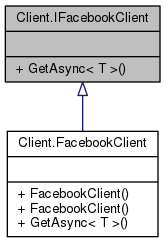
\includegraphics[width=196pt]{interface_client_1_1_i_facebook_client__inherit__graph}
\end{center}
\end{figure}


Collaboration diagram for Client.\+I\+Facebook\+Client\+:
\nopagebreak
\begin{figure}[H]
\begin{center}
\leavevmode
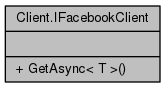
\includegraphics[width=196pt]{interface_client_1_1_i_facebook_client__coll__graph}
\end{center}
\end{figure}
\subsection*{Public Member Functions}
\begin{DoxyCompactItemize}
\item 
Task$<$ T $>$ \hyperlink{interface_client_1_1_i_facebook_client_adcc547867f709ce07787df58233c0b85}{Get\+Async$<$ T $>$} (string access\+Token, string endpoint, string pageview, string args=null)
\end{DoxyCompactItemize}


\subsection{Detailed Description}
Interface Framework for \hyperlink{class_client_1_1_facebook_client}{Facebook\+Client} 



Definition at line 15 of file Facebook\+Client.\+cs.



\subsection{Member Function Documentation}
\index{Client\+::\+I\+Facebook\+Client@{Client\+::\+I\+Facebook\+Client}!Get\+Async$<$ T $>$@{Get\+Async$<$ T $>$}}
\index{Get\+Async$<$ T $>$@{Get\+Async$<$ T $>$}!Client\+::\+I\+Facebook\+Client@{Client\+::\+I\+Facebook\+Client}}
\subsubsection[{\texorpdfstring{Get\+Async$<$ T $>$(string access\+Token, string endpoint, string pageview, string args=null)}{GetAsync< T >(string accessToken, string endpoint, string pageview, string args=null)}}]{\setlength{\rightskip}{0pt plus 5cm}Task$<$T$>$ Client.\+I\+Facebook\+Client.\+Get\+Async$<$ T $>$ (
\begin{DoxyParamCaption}
\item[{string}]{access\+Token, }
\item[{string}]{endpoint, }
\item[{string}]{pageview, }
\item[{string}]{args = {\ttfamily null}}
\end{DoxyParamCaption}
)}\hypertarget{interface_client_1_1_i_facebook_client_adcc547867f709ce07787df58233c0b85}{}\label{interface_client_1_1_i_facebook_client_adcc547867f709ce07787df58233c0b85}


Implemented in \hyperlink{class_client_1_1_facebook_client_aa8feb74481610d6e45da94798656adca}{Client.\+Facebook\+Client}.



The documentation for this interface was generated from the following file\+:\begin{DoxyCompactItemize}
\item 
Facebook\+Application/\+Client/\hyperlink{_facebook_client_8cs}{Facebook\+Client.\+cs}\end{DoxyCompactItemize}

\hypertarget{interface_operations_1_1_data_operations_1_1_i_populate_n_e_t_object}{}\section{Operations.\+Data\+Operations.\+I\+Populate\+N\+E\+T\+Object Interface Reference}
\label{interface_operations_1_1_data_operations_1_1_i_populate_n_e_t_object}\index{Operations.\+Data\+Operations.\+I\+Populate\+N\+E\+T\+Object@{Operations.\+Data\+Operations.\+I\+Populate\+N\+E\+T\+Object}}


Inheritance diagram for Operations.\+Data\+Operations.\+I\+Populate\+N\+E\+T\+Object\+:
\nopagebreak
\begin{figure}[H]
\begin{center}
\leavevmode
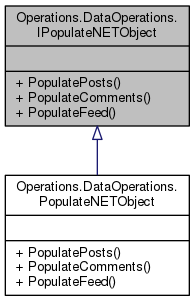
\includegraphics[width=218pt]{interface_operations_1_1_data_operations_1_1_i_populate_n_e_t_object__inherit__graph}
\end{center}
\end{figure}


Collaboration diagram for Operations.\+Data\+Operations.\+I\+Populate\+N\+E\+T\+Object\+:
\nopagebreak
\begin{figure}[H]
\begin{center}
\leavevmode
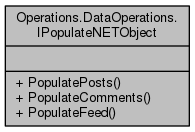
\includegraphics[width=218pt]{interface_operations_1_1_data_operations_1_1_i_populate_n_e_t_object__coll__graph}
\end{center}
\end{figure}
\subsection*{Public Member Functions}
\begin{DoxyCompactItemize}
\item 
List$<$ \hyperlink{class_data_1_1_facebook_objects_1_1_post}{Post} $>$ \hyperlink{interface_operations_1_1_data_operations_1_1_i_populate_n_e_t_object_a404db639d5476203f9aabfe79d10c6ab}{Populate\+Posts} (dynamic response)
\item 
List$<$ \hyperlink{class_data_1_1_facebook_objects_1_1_comment}{Comment} $>$ \hyperlink{interface_operations_1_1_data_operations_1_1_i_populate_n_e_t_object_ac71d6a76fa87075a7bee781e0e82aa3e}{Populate\+Comments} (dynamic response, string origin\+\_\+type)
\item 
List$<$ \hyperlink{class_data_1_1_facebook_objects_1_1_feed}{Feed} $>$ \hyperlink{interface_operations_1_1_data_operations_1_1_i_populate_n_e_t_object_a09f34c1fdef92c7c02f6ae8b47caef89}{Populate\+Feed} (dynamic response)
\end{DoxyCompactItemize}


\subsection{Detailed Description}


Definition at line 12 of file Populate\+N\+E\+T\+Object.\+cs.



\subsection{Member Function Documentation}
\index{Operations\+::\+Data\+Operations\+::\+I\+Populate\+N\+E\+T\+Object@{Operations\+::\+Data\+Operations\+::\+I\+Populate\+N\+E\+T\+Object}!Populate\+Comments@{Populate\+Comments}}
\index{Populate\+Comments@{Populate\+Comments}!Operations\+::\+Data\+Operations\+::\+I\+Populate\+N\+E\+T\+Object@{Operations\+::\+Data\+Operations\+::\+I\+Populate\+N\+E\+T\+Object}}
\subsubsection[{\texorpdfstring{Populate\+Comments(dynamic response, string origin\+\_\+type)}{PopulateComments(dynamic response, string origin_type)}}]{\setlength{\rightskip}{0pt plus 5cm}List$<${\bf Comment}$>$ Operations.\+Data\+Operations.\+I\+Populate\+N\+E\+T\+Object.\+Populate\+Comments (
\begin{DoxyParamCaption}
\item[{dynamic}]{response, }
\item[{string}]{origin\+\_\+type}
\end{DoxyParamCaption}
)}\hypertarget{interface_operations_1_1_data_operations_1_1_i_populate_n_e_t_object_ac71d6a76fa87075a7bee781e0e82aa3e}{}\label{interface_operations_1_1_data_operations_1_1_i_populate_n_e_t_object_ac71d6a76fa87075a7bee781e0e82aa3e}


Implemented in \hyperlink{class_operations_1_1_data_operations_1_1_populate_n_e_t_object_a6573ae438326c9fb036ba38af6cb0d16}{Operations.\+Data\+Operations.\+Populate\+N\+E\+T\+Object}.

\index{Operations\+::\+Data\+Operations\+::\+I\+Populate\+N\+E\+T\+Object@{Operations\+::\+Data\+Operations\+::\+I\+Populate\+N\+E\+T\+Object}!Populate\+Feed@{Populate\+Feed}}
\index{Populate\+Feed@{Populate\+Feed}!Operations\+::\+Data\+Operations\+::\+I\+Populate\+N\+E\+T\+Object@{Operations\+::\+Data\+Operations\+::\+I\+Populate\+N\+E\+T\+Object}}
\subsubsection[{\texorpdfstring{Populate\+Feed(dynamic response)}{PopulateFeed(dynamic response)}}]{\setlength{\rightskip}{0pt plus 5cm}List$<${\bf Feed}$>$ Operations.\+Data\+Operations.\+I\+Populate\+N\+E\+T\+Object.\+Populate\+Feed (
\begin{DoxyParamCaption}
\item[{dynamic}]{response}
\end{DoxyParamCaption}
)}\hypertarget{interface_operations_1_1_data_operations_1_1_i_populate_n_e_t_object_a09f34c1fdef92c7c02f6ae8b47caef89}{}\label{interface_operations_1_1_data_operations_1_1_i_populate_n_e_t_object_a09f34c1fdef92c7c02f6ae8b47caef89}


Implemented in \hyperlink{class_operations_1_1_data_operations_1_1_populate_n_e_t_object_a31da696e614215afced22da40a5b3f20}{Operations.\+Data\+Operations.\+Populate\+N\+E\+T\+Object}.

\index{Operations\+::\+Data\+Operations\+::\+I\+Populate\+N\+E\+T\+Object@{Operations\+::\+Data\+Operations\+::\+I\+Populate\+N\+E\+T\+Object}!Populate\+Posts@{Populate\+Posts}}
\index{Populate\+Posts@{Populate\+Posts}!Operations\+::\+Data\+Operations\+::\+I\+Populate\+N\+E\+T\+Object@{Operations\+::\+Data\+Operations\+::\+I\+Populate\+N\+E\+T\+Object}}
\subsubsection[{\texorpdfstring{Populate\+Posts(dynamic response)}{PopulatePosts(dynamic response)}}]{\setlength{\rightskip}{0pt plus 5cm}List$<${\bf Post}$>$ Operations.\+Data\+Operations.\+I\+Populate\+N\+E\+T\+Object.\+Populate\+Posts (
\begin{DoxyParamCaption}
\item[{dynamic}]{response}
\end{DoxyParamCaption}
)}\hypertarget{interface_operations_1_1_data_operations_1_1_i_populate_n_e_t_object_a404db639d5476203f9aabfe79d10c6ab}{}\label{interface_operations_1_1_data_operations_1_1_i_populate_n_e_t_object_a404db639d5476203f9aabfe79d10c6ab}


Implemented in \hyperlink{class_operations_1_1_data_operations_1_1_populate_n_e_t_object_a780372790782b34a234524055c1afec5}{Operations.\+Data\+Operations.\+Populate\+N\+E\+T\+Object}.



The documentation for this interface was generated from the following file\+:\begin{DoxyCompactItemize}
\item 
Facebook\+Application/\+Operations/\+Data\+Operations/\hyperlink{_populate_n_e_t_object_8cs}{Populate\+N\+E\+T\+Object.\+cs}\end{DoxyCompactItemize}

\hypertarget{interface_services_1_1_i_text_reader}{}\section{Services.\+I\+Text\+Reader Interface Reference}
\label{interface_services_1_1_i_text_reader}\index{Services.\+I\+Text\+Reader@{Services.\+I\+Text\+Reader}}


Inheritance diagram for Services.\+I\+Text\+Reader\+:
\nopagebreak
\begin{figure}[H]
\begin{center}
\leavevmode
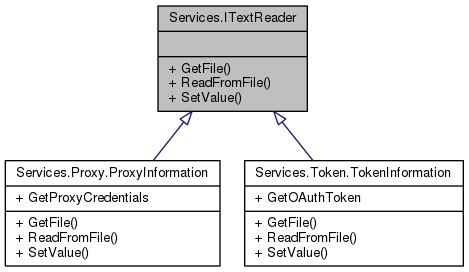
\includegraphics[width=350pt]{interface_services_1_1_i_text_reader__inherit__graph}
\end{center}
\end{figure}


Collaboration diagram for Services.\+I\+Text\+Reader\+:
\nopagebreak
\begin{figure}[H]
\begin{center}
\leavevmode
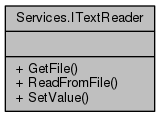
\includegraphics[width=192pt]{interface_services_1_1_i_text_reader__coll__graph}
\end{center}
\end{figure}
\subsection*{Public Member Functions}
\begin{DoxyCompactItemize}
\item 
string\mbox{[}$\,$\mbox{]} \hyperlink{interface_services_1_1_i_text_reader_a729359f5178930c633a7d0480041638a}{Get\+File} ()
\begin{DoxyCompactList}\small\item\em Identify path to token file. Method to be used as submethod -\/ therefore private scope. \end{DoxyCompactList}\item 
void \hyperlink{interface_services_1_1_i_text_reader_ab635d59d4de79bf41ffe7a184473f416}{Read\+From\+File} (Text\+Reader reader)
\begin{DoxyCompactList}\small\item\em Read relevant content from file \end{DoxyCompactList}\item 
void \hyperlink{interface_services_1_1_i_text_reader_a670edc32225de1bcaf9942b4acc1edaf}{Set\+Value} ()
\begin{DoxyCompactList}\small\item\em Makes the value accessible \end{DoxyCompactList}\end{DoxyCompactItemize}


\subsection{Detailed Description}


Definition at line 6 of file I\+Text\+Reader.\+cs.



\subsection{Member Function Documentation}
\index{Services\+::\+I\+Text\+Reader@{Services\+::\+I\+Text\+Reader}!Get\+File@{Get\+File}}
\index{Get\+File@{Get\+File}!Services\+::\+I\+Text\+Reader@{Services\+::\+I\+Text\+Reader}}
\subsubsection[{\texorpdfstring{Get\+File()}{GetFile()}}]{\setlength{\rightskip}{0pt plus 5cm}string \mbox{[}$\,$\mbox{]} Services.\+I\+Text\+Reader.\+Get\+File (
\begin{DoxyParamCaption}
{}
\end{DoxyParamCaption}
)}\hypertarget{interface_services_1_1_i_text_reader_a729359f5178930c633a7d0480041638a}{}\label{interface_services_1_1_i_text_reader_a729359f5178930c633a7d0480041638a}


Identify path to token file. Method to be used as submethod -\/ therefore private scope. 



Implemented in \hyperlink{class_services_1_1_token_1_1_token_information_a37295436ba6b0c749486fcb647fcd904}{Services.\+Token.\+Token\+Information}, and \hyperlink{class_services_1_1_proxy_1_1_proxy_information_ac775377976e6b9a38de042bf29440174}{Services.\+Proxy.\+Proxy\+Information}.

\index{Services\+::\+I\+Text\+Reader@{Services\+::\+I\+Text\+Reader}!Read\+From\+File@{Read\+From\+File}}
\index{Read\+From\+File@{Read\+From\+File}!Services\+::\+I\+Text\+Reader@{Services\+::\+I\+Text\+Reader}}
\subsubsection[{\texorpdfstring{Read\+From\+File(\+Text\+Reader reader)}{ReadFromFile(TextReader reader)}}]{\setlength{\rightskip}{0pt plus 5cm}void Services.\+I\+Text\+Reader.\+Read\+From\+File (
\begin{DoxyParamCaption}
\item[{Text\+Reader}]{reader}
\end{DoxyParamCaption}
)}\hypertarget{interface_services_1_1_i_text_reader_ab635d59d4de79bf41ffe7a184473f416}{}\label{interface_services_1_1_i_text_reader_ab635d59d4de79bf41ffe7a184473f416}


Read relevant content from file 


\begin{DoxyParams}{Parameters}
{\em reader} & Text\+Reader Objecet.\\
\hline
\end{DoxyParams}


Implemented in \hyperlink{class_services_1_1_token_1_1_token_information_ac080b926c4adadd033ebad6cea64baf4}{Services.\+Token.\+Token\+Information}, and \hyperlink{class_services_1_1_proxy_1_1_proxy_information_abb9b80a08af3fd6458a68ad258113664}{Services.\+Proxy.\+Proxy\+Information}.

\index{Services\+::\+I\+Text\+Reader@{Services\+::\+I\+Text\+Reader}!Set\+Value@{Set\+Value}}
\index{Set\+Value@{Set\+Value}!Services\+::\+I\+Text\+Reader@{Services\+::\+I\+Text\+Reader}}
\subsubsection[{\texorpdfstring{Set\+Value()}{SetValue()}}]{\setlength{\rightskip}{0pt plus 5cm}void Services.\+I\+Text\+Reader.\+Set\+Value (
\begin{DoxyParamCaption}
{}
\end{DoxyParamCaption}
)}\hypertarget{interface_services_1_1_i_text_reader_a670edc32225de1bcaf9942b4acc1edaf}{}\label{interface_services_1_1_i_text_reader_a670edc32225de1bcaf9942b4acc1edaf}


Makes the value accessible 



Implemented in \hyperlink{class_services_1_1_token_1_1_token_information_a2cdb068d0ace07409c398e3c40c5b84d}{Services.\+Token.\+Token\+Information}, and \hyperlink{class_services_1_1_proxy_1_1_proxy_information_aff83ebf7729262cfe2840c26a9ef73f0}{Services.\+Proxy.\+Proxy\+Information}.



The documentation for this interface was generated from the following file\+:\begin{DoxyCompactItemize}
\item 
Facebook\+Application/\+Services/\hyperlink{_i_text_reader_8cs}{I\+Text\+Reader.\+cs}\end{DoxyCompactItemize}

\hypertarget{class_g_u_i_1_1_main_class}{}\section{G\+U\+I.\+Main\+Class Class Reference}
\label{class_g_u_i_1_1_main_class}\index{G\+U\+I.\+Main\+Class@{G\+U\+I.\+Main\+Class}}


Collaboration diagram for G\+U\+I.\+Main\+Class\+:
\nopagebreak
\begin{figure}[H]
\begin{center}
\leavevmode
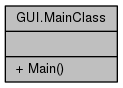
\includegraphics[width=164pt]{class_g_u_i_1_1_main_class__coll__graph}
\end{center}
\end{figure}
\subsection*{Static Public Member Functions}
\begin{DoxyCompactItemize}
\item 
static void \hyperlink{class_g_u_i_1_1_main_class_a357f0ac132ec52fb982d3902b6cfce00}{Main} (string\mbox{[}$\,$\mbox{]} args)
\end{DoxyCompactItemize}


\subsection{Detailed Description}


Definition at line 6 of file Program.\+cs.



\subsection{Member Function Documentation}
\index{G\+U\+I\+::\+Main\+Class@{G\+U\+I\+::\+Main\+Class}!Main@{Main}}
\index{Main@{Main}!G\+U\+I\+::\+Main\+Class@{G\+U\+I\+::\+Main\+Class}}
\subsubsection[{\texorpdfstring{Main(string[] args)}{Main(string[] args)}}]{\setlength{\rightskip}{0pt plus 5cm}static void G\+U\+I.\+Main\+Class.\+Main (
\begin{DoxyParamCaption}
\item[{string\mbox{[}$\,$\mbox{]}}]{args}
\end{DoxyParamCaption}
)\hspace{0.3cm}{\ttfamily [static]}}\hypertarget{class_g_u_i_1_1_main_class_a357f0ac132ec52fb982d3902b6cfce00}{}\label{class_g_u_i_1_1_main_class_a357f0ac132ec52fb982d3902b6cfce00}


Definition at line 8 of file Program.\+cs.



The documentation for this class was generated from the following file\+:\begin{DoxyCompactItemize}
\item 
Facebook\+Application/\+G\+U\+I/\hyperlink{_g_u_i_2_program_8cs}{Program.\+cs}\end{DoxyCompactItemize}

\hypertarget{class_main_window}{}\section{Main\+Window Class Reference}
\label{class_main_window}\index{Main\+Window@{Main\+Window}}


Inheritance diagram for Main\+Window\+:
\nopagebreak
\begin{figure}[H]
\begin{center}
\leavevmode
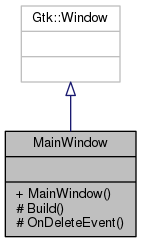
\includegraphics[width=178pt]{class_main_window__inherit__graph}
\end{center}
\end{figure}


Collaboration diagram for Main\+Window\+:
\nopagebreak
\begin{figure}[H]
\begin{center}
\leavevmode
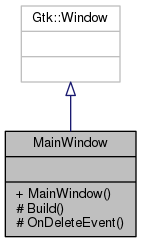
\includegraphics[width=178pt]{class_main_window__coll__graph}
\end{center}
\end{figure}
\subsection*{Public Member Functions}
\begin{DoxyCompactItemize}
\item 
\hyperlink{class_main_window_af607d50e4d1b04d3c494661489283f45}{Main\+Window} ()
\end{DoxyCompactItemize}
\subsection*{Protected Member Functions}
\begin{DoxyCompactItemize}
\item 
virtual void \hyperlink{class_main_window_a952a77b964806830814cf4cdfbb2f0b9}{Build} ()
\item 
void \hyperlink{class_main_window_a64bdcb29cebb58957790da1ee2733fe1}{On\+Delete\+Event} (object sender, Delete\+Event\+Args a)
\end{DoxyCompactItemize}


\subsection{Detailed Description}


Definition at line 4 of file Main\+Window.\+cs.



\subsection{Constructor \& Destructor Documentation}
\index{Main\+Window@{Main\+Window}!Main\+Window@{Main\+Window}}
\index{Main\+Window@{Main\+Window}!Main\+Window@{Main\+Window}}
\subsubsection[{\texorpdfstring{Main\+Window()}{MainWindow()}}]{\setlength{\rightskip}{0pt plus 5cm}Main\+Window.\+Main\+Window (
\begin{DoxyParamCaption}
{}
\end{DoxyParamCaption}
)}\hypertarget{class_main_window_af607d50e4d1b04d3c494661489283f45}{}\label{class_main_window_af607d50e4d1b04d3c494661489283f45}


Definition at line 6 of file Main\+Window.\+cs.



References Build().



Here is the call graph for this function\+:
\nopagebreak
\begin{figure}[H]
\begin{center}
\leavevmode
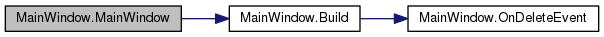
\includegraphics[width=350pt]{class_main_window_af607d50e4d1b04d3c494661489283f45_cgraph}
\end{center}
\end{figure}




\subsection{Member Function Documentation}
\index{Main\+Window@{Main\+Window}!Build@{Build}}
\index{Build@{Build}!Main\+Window@{Main\+Window}}
\subsubsection[{\texorpdfstring{Build()}{Build()}}]{\setlength{\rightskip}{0pt plus 5cm}virtual void Main\+Window.\+Build (
\begin{DoxyParamCaption}
{}
\end{DoxyParamCaption}
)\hspace{0.3cm}{\ttfamily [protected]}, {\ttfamily [virtual]}}\hypertarget{class_main_window_a952a77b964806830814cf4cdfbb2f0b9}{}\label{class_main_window_a952a77b964806830814cf4cdfbb2f0b9}


Definition at line 6 of file Main\+Window.\+cs.



References On\+Delete\+Event().



Referenced by Main\+Window().



Here is the call graph for this function\+:
\nopagebreak
\begin{figure}[H]
\begin{center}
\leavevmode
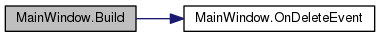
\includegraphics[width=350pt]{class_main_window_a952a77b964806830814cf4cdfbb2f0b9_cgraph}
\end{center}
\end{figure}




Here is the caller graph for this function\+:
\nopagebreak
\begin{figure}[H]
\begin{center}
\leavevmode
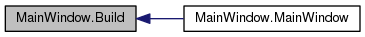
\includegraphics[width=346pt]{class_main_window_a952a77b964806830814cf4cdfbb2f0b9_icgraph}
\end{center}
\end{figure}


\index{Main\+Window@{Main\+Window}!On\+Delete\+Event@{On\+Delete\+Event}}
\index{On\+Delete\+Event@{On\+Delete\+Event}!Main\+Window@{Main\+Window}}
\subsubsection[{\texorpdfstring{On\+Delete\+Event(object sender, Delete\+Event\+Args a)}{OnDeleteEvent(object sender, DeleteEventArgs a)}}]{\setlength{\rightskip}{0pt plus 5cm}void Main\+Window.\+On\+Delete\+Event (
\begin{DoxyParamCaption}
\item[{object}]{sender, }
\item[{Delete\+Event\+Args}]{a}
\end{DoxyParamCaption}
)\hspace{0.3cm}{\ttfamily [protected]}}\hypertarget{class_main_window_a64bdcb29cebb58957790da1ee2733fe1}{}\label{class_main_window_a64bdcb29cebb58957790da1ee2733fe1}


Definition at line 11 of file Main\+Window.\+cs.



Referenced by Build().



Here is the caller graph for this function\+:
\nopagebreak
\begin{figure}[H]
\begin{center}
\leavevmode
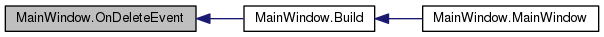
\includegraphics[width=350pt]{class_main_window_a64bdcb29cebb58957790da1ee2733fe1_icgraph}
\end{center}
\end{figure}




The documentation for this class was generated from the following file\+:\begin{DoxyCompactItemize}
\item 
Facebook\+Application/\+G\+U\+I/gtk-\/gui/\hyperlink{gtk-gui_2_main_window_8cs}{Main\+Window.\+cs}\end{DoxyCompactItemize}

\hypertarget{class_operations_1_1_data_operations_1_1_populate_n_e_t_object}{}\section{Operations.\+Data\+Operations.\+Populate\+N\+E\+T\+Object Class Reference}
\label{class_operations_1_1_data_operations_1_1_populate_n_e_t_object}\index{Operations.\+Data\+Operations.\+Populate\+N\+E\+T\+Object@{Operations.\+Data\+Operations.\+Populate\+N\+E\+T\+Object}}


Class with methods for populating custom object-\/types  




Inheritance diagram for Operations.\+Data\+Operations.\+Populate\+N\+E\+T\+Object\+:
\nopagebreak
\begin{figure}[H]
\begin{center}
\leavevmode
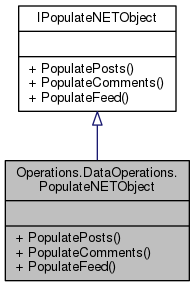
\includegraphics[width=218pt]{class_operations_1_1_data_operations_1_1_populate_n_e_t_object__inherit__graph}
\end{center}
\end{figure}


Collaboration diagram for Operations.\+Data\+Operations.\+Populate\+N\+E\+T\+Object\+:
\nopagebreak
\begin{figure}[H]
\begin{center}
\leavevmode
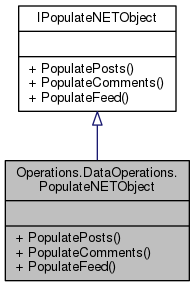
\includegraphics[width=218pt]{class_operations_1_1_data_operations_1_1_populate_n_e_t_object__coll__graph}
\end{center}
\end{figure}
\subsection*{Public Member Functions}
\begin{DoxyCompactItemize}
\item 
List$<$ \hyperlink{class_data_1_1_facebook_objects_1_1_post}{Post} $>$ \hyperlink{class_operations_1_1_data_operations_1_1_populate_n_e_t_object_a780372790782b34a234524055c1afec5}{Populate\+Posts} (dynamic response)
\begin{DoxyCompactList}\small\item\em Populates a list of Post-\/objects \end{DoxyCompactList}\item 
List$<$ \hyperlink{class_data_1_1_facebook_objects_1_1_comment}{Comment} $>$ \hyperlink{class_operations_1_1_data_operations_1_1_populate_n_e_t_object_a6573ae438326c9fb036ba38af6cb0d16}{Populate\+Comments} (dynamic response, string origin\+\_\+type)
\begin{DoxyCompactList}\small\item\em Populates a list of Comment-\/objects \end{DoxyCompactList}\item 
List$<$ \hyperlink{class_data_1_1_facebook_objects_1_1_feed}{Feed} $>$ \hyperlink{class_operations_1_1_data_operations_1_1_populate_n_e_t_object_a31da696e614215afced22da40a5b3f20}{Populate\+Feed} (dynamic response)
\begin{DoxyCompactList}\small\item\em Populates a list of Feed objects \end{DoxyCompactList}\end{DoxyCompactItemize}


\subsection{Detailed Description}
Class with methods for populating custom object-\/types 



Definition at line 22 of file Populate\+N\+E\+T\+Object.\+cs.



\subsection{Member Function Documentation}
\index{Operations\+::\+Data\+Operations\+::\+Populate\+N\+E\+T\+Object@{Operations\+::\+Data\+Operations\+::\+Populate\+N\+E\+T\+Object}!Populate\+Comments@{Populate\+Comments}}
\index{Populate\+Comments@{Populate\+Comments}!Operations\+::\+Data\+Operations\+::\+Populate\+N\+E\+T\+Object@{Operations\+::\+Data\+Operations\+::\+Populate\+N\+E\+T\+Object}}
\subsubsection[{\texorpdfstring{Populate\+Comments(dynamic response, string origin\+\_\+type)}{PopulateComments(dynamic response, string origin_type)}}]{\setlength{\rightskip}{0pt plus 5cm}List$<${\bf Comment}$>$ Operations.\+Data\+Operations.\+Populate\+N\+E\+T\+Object.\+Populate\+Comments (
\begin{DoxyParamCaption}
\item[{dynamic}]{response, }
\item[{string}]{origin\+\_\+type}
\end{DoxyParamCaption}
)}\hypertarget{class_operations_1_1_data_operations_1_1_populate_n_e_t_object_a6573ae438326c9fb036ba38af6cb0d16}{}\label{class_operations_1_1_data_operations_1_1_populate_n_e_t_object_a6573ae438326c9fb036ba38af6cb0d16}


Populates a list of Comment-\/objects 

\begin{DoxyReturn}{Returns}
A list of Comment-\/objects
\end{DoxyReturn}

\begin{DoxyParams}{Parameters}
{\em response} & A list of dynamic objects from Get\+Async.\\
\hline
\end{DoxyParams}


Implements \hyperlink{interface_operations_1_1_data_operations_1_1_i_populate_n_e_t_object_ac71d6a76fa87075a7bee781e0e82aa3e}{Operations.\+Data\+Operations.\+I\+Populate\+N\+E\+T\+Object}.



Definition at line 82 of file Populate\+N\+E\+T\+Object.\+cs.



References Data.\+Facebook\+Objects.\+Application.\+category, Data.\+Facebook\+Objects.\+Comment.\+created\+\_\+time, and Data.\+Facebook\+Objects.\+Comment.\+message.

\index{Operations\+::\+Data\+Operations\+::\+Populate\+N\+E\+T\+Object@{Operations\+::\+Data\+Operations\+::\+Populate\+N\+E\+T\+Object}!Populate\+Feed@{Populate\+Feed}}
\index{Populate\+Feed@{Populate\+Feed}!Operations\+::\+Data\+Operations\+::\+Populate\+N\+E\+T\+Object@{Operations\+::\+Data\+Operations\+::\+Populate\+N\+E\+T\+Object}}
\subsubsection[{\texorpdfstring{Populate\+Feed(dynamic response)}{PopulateFeed(dynamic response)}}]{\setlength{\rightskip}{0pt plus 5cm}List$<${\bf Feed}$>$ Operations.\+Data\+Operations.\+Populate\+N\+E\+T\+Object.\+Populate\+Feed (
\begin{DoxyParamCaption}
\item[{dynamic}]{response}
\end{DoxyParamCaption}
)}\hypertarget{class_operations_1_1_data_operations_1_1_populate_n_e_t_object_a31da696e614215afced22da40a5b3f20}{}\label{class_operations_1_1_data_operations_1_1_populate_n_e_t_object_a31da696e614215afced22da40a5b3f20}


Populates a list of Feed objects 

\begin{DoxyReturn}{Returns}
A list of Feed objects
\end{DoxyReturn}

\begin{DoxyParams}{Parameters}
{\em response} & A list of dynamic objects from Get\+Async.\\
\hline
\end{DoxyParams}


Implements \hyperlink{interface_operations_1_1_data_operations_1_1_i_populate_n_e_t_object_a09f34c1fdef92c7c02f6ae8b47caef89}{Operations.\+Data\+Operations.\+I\+Populate\+N\+E\+T\+Object}.



Definition at line 170 of file Populate\+N\+E\+T\+Object.\+cs.



References Data.\+Facebook\+Objects.\+Feed.\+message.

\index{Operations\+::\+Data\+Operations\+::\+Populate\+N\+E\+T\+Object@{Operations\+::\+Data\+Operations\+::\+Populate\+N\+E\+T\+Object}!Populate\+Posts@{Populate\+Posts}}
\index{Populate\+Posts@{Populate\+Posts}!Operations\+::\+Data\+Operations\+::\+Populate\+N\+E\+T\+Object@{Operations\+::\+Data\+Operations\+::\+Populate\+N\+E\+T\+Object}}
\subsubsection[{\texorpdfstring{Populate\+Posts(dynamic response)}{PopulatePosts(dynamic response)}}]{\setlength{\rightskip}{0pt plus 5cm}List$<${\bf Post}$>$ Operations.\+Data\+Operations.\+Populate\+N\+E\+T\+Object.\+Populate\+Posts (
\begin{DoxyParamCaption}
\item[{dynamic}]{response}
\end{DoxyParamCaption}
)}\hypertarget{class_operations_1_1_data_operations_1_1_populate_n_e_t_object_a780372790782b34a234524055c1afec5}{}\label{class_operations_1_1_data_operations_1_1_populate_n_e_t_object_a780372790782b34a234524055c1afec5}


Populates a list of Post-\/objects 

\begin{DoxyReturn}{Returns}
A list of Post-\/objects
\end{DoxyReturn}

\begin{DoxyParams}{Parameters}
{\em response} & A list of dynamic objects from Get\+Async.\\
\hline
\end{DoxyParams}


Implements \hyperlink{interface_operations_1_1_data_operations_1_1_i_populate_n_e_t_object_a404db639d5476203f9aabfe79d10c6ab}{Operations.\+Data\+Operations.\+I\+Populate\+N\+E\+T\+Object}.



Definition at line 29 of file Populate\+N\+E\+T\+Object.\+cs.



References Data.\+Facebook\+Objects.\+Post.\+status\+\_\+type.



The documentation for this class was generated from the following file\+:\begin{DoxyCompactItemize}
\item 
Facebook\+Application/\+Operations/\+Data\+Operations/\hyperlink{_populate_n_e_t_object_8cs}{Populate\+N\+E\+T\+Object.\+cs}\end{DoxyCompactItemize}

\hypertarget{class_data_1_1_facebook_objects_1_1_post}{}\section{Data.\+Facebook\+Objects.\+Post Class Reference}
\label{class_data_1_1_facebook_objects_1_1_post}\index{Data.\+Facebook\+Objects.\+Post@{Data.\+Facebook\+Objects.\+Post}}


Collaboration diagram for Data.\+Facebook\+Objects.\+Post\+:
\nopagebreak
\begin{figure}[H]
\begin{center}
\leavevmode
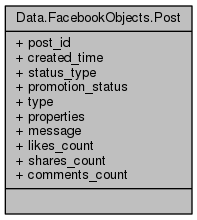
\includegraphics[width=220pt]{class_data_1_1_facebook_objects_1_1_post__coll__graph}
\end{center}
\end{figure}
\subsection*{Properties}
\begin{DoxyCompactItemize}
\item 
string \hyperlink{class_data_1_1_facebook_objects_1_1_post_aee4b1dee4da506a8dec173c1e5742e07}{post\+\_\+id}\hspace{0.3cm}{\ttfamily  \mbox{[}get, set\mbox{]}}
\item 
Date\+Time \hyperlink{class_data_1_1_facebook_objects_1_1_post_a788a4e4d88bd8abe96bcbdb4143a0349}{created\+\_\+time}\hspace{0.3cm}{\ttfamily  \mbox{[}get, set\mbox{]}}
\item 
string \hyperlink{class_data_1_1_facebook_objects_1_1_post_a108de96063725263fdd8a0df92f110ab}{status\+\_\+type}\hspace{0.3cm}{\ttfamily  \mbox{[}get, set\mbox{]}}
\item 
string \hyperlink{class_data_1_1_facebook_objects_1_1_post_a4fbe2ab37ecd327a18c5f287d68c9053}{promotion\+\_\+status}\hspace{0.3cm}{\ttfamily  \mbox{[}get, set\mbox{]}}
\item 
string \hyperlink{class_data_1_1_facebook_objects_1_1_post_aa2861fcd6537791f9d5f518af2675992}{type}\hspace{0.3cm}{\ttfamily  \mbox{[}get, set\mbox{]}}
\item 
\hyperlink{class_data_1_1_facebook_objects_1_1_properties}{Properties} \hyperlink{class_data_1_1_facebook_objects_1_1_post_ab2e3fc0d8e9b75295bdc4ea4a4431ec7}{properties}\hspace{0.3cm}{\ttfamily  \mbox{[}get, set\mbox{]}}
\item 
string \hyperlink{class_data_1_1_facebook_objects_1_1_post_a1073224aa852149b7109dea0cf119492}{message}\hspace{0.3cm}{\ttfamily  \mbox{[}get, set\mbox{]}}
\item 
int \hyperlink{class_data_1_1_facebook_objects_1_1_post_a38a034ec87f87cf493b855155d0195cd}{likes\+\_\+count}\hspace{0.3cm}{\ttfamily  \mbox{[}get, set\mbox{]}}
\item 
int \hyperlink{class_data_1_1_facebook_objects_1_1_post_aaa87c76997dad586306046b5f3299978}{shares\+\_\+count}\hspace{0.3cm}{\ttfamily  \mbox{[}get, set\mbox{]}}
\item 
int \hyperlink{class_data_1_1_facebook_objects_1_1_post_af17bbc52c65a9b92fa4a6ff4f41f85d7}{comments\+\_\+count}\hspace{0.3cm}{\ttfamily  \mbox{[}get, set\mbox{]}}
\end{DoxyCompactItemize}


\subsection{Detailed Description}


Definition at line 7 of file Post.\+cs.



\subsection{Property Documentation}
\index{Data\+::\+Facebook\+Objects\+::\+Post@{Data\+::\+Facebook\+Objects\+::\+Post}!comments\+\_\+count@{comments\+\_\+count}}
\index{comments\+\_\+count@{comments\+\_\+count}!Data\+::\+Facebook\+Objects\+::\+Post@{Data\+::\+Facebook\+Objects\+::\+Post}}
\subsubsection[{\texorpdfstring{comments\+\_\+count}{comments_count}}]{\setlength{\rightskip}{0pt plus 5cm}int Data.\+Facebook\+Objects.\+Post.\+comments\+\_\+count\hspace{0.3cm}{\ttfamily [get]}, {\ttfamily [set]}}\hypertarget{class_data_1_1_facebook_objects_1_1_post_af17bbc52c65a9b92fa4a6ff4f41f85d7}{}\label{class_data_1_1_facebook_objects_1_1_post_af17bbc52c65a9b92fa4a6ff4f41f85d7}


Definition at line 18 of file Post.\+cs.

\index{Data\+::\+Facebook\+Objects\+::\+Post@{Data\+::\+Facebook\+Objects\+::\+Post}!created\+\_\+time@{created\+\_\+time}}
\index{created\+\_\+time@{created\+\_\+time}!Data\+::\+Facebook\+Objects\+::\+Post@{Data\+::\+Facebook\+Objects\+::\+Post}}
\subsubsection[{\texorpdfstring{created\+\_\+time}{created_time}}]{\setlength{\rightskip}{0pt plus 5cm}Date\+Time Data.\+Facebook\+Objects.\+Post.\+created\+\_\+time\hspace{0.3cm}{\ttfamily [get]}, {\ttfamily [set]}}\hypertarget{class_data_1_1_facebook_objects_1_1_post_a788a4e4d88bd8abe96bcbdb4143a0349}{}\label{class_data_1_1_facebook_objects_1_1_post_a788a4e4d88bd8abe96bcbdb4143a0349}


Definition at line 10 of file Post.\+cs.

\index{Data\+::\+Facebook\+Objects\+::\+Post@{Data\+::\+Facebook\+Objects\+::\+Post}!likes\+\_\+count@{likes\+\_\+count}}
\index{likes\+\_\+count@{likes\+\_\+count}!Data\+::\+Facebook\+Objects\+::\+Post@{Data\+::\+Facebook\+Objects\+::\+Post}}
\subsubsection[{\texorpdfstring{likes\+\_\+count}{likes_count}}]{\setlength{\rightskip}{0pt plus 5cm}int Data.\+Facebook\+Objects.\+Post.\+likes\+\_\+count\hspace{0.3cm}{\ttfamily [get]}, {\ttfamily [set]}}\hypertarget{class_data_1_1_facebook_objects_1_1_post_a38a034ec87f87cf493b855155d0195cd}{}\label{class_data_1_1_facebook_objects_1_1_post_a38a034ec87f87cf493b855155d0195cd}


Definition at line 16 of file Post.\+cs.

\index{Data\+::\+Facebook\+Objects\+::\+Post@{Data\+::\+Facebook\+Objects\+::\+Post}!message@{message}}
\index{message@{message}!Data\+::\+Facebook\+Objects\+::\+Post@{Data\+::\+Facebook\+Objects\+::\+Post}}
\subsubsection[{\texorpdfstring{message}{message}}]{\setlength{\rightskip}{0pt plus 5cm}string Data.\+Facebook\+Objects.\+Post.\+message\hspace{0.3cm}{\ttfamily [get]}, {\ttfamily [set]}}\hypertarget{class_data_1_1_facebook_objects_1_1_post_a1073224aa852149b7109dea0cf119492}{}\label{class_data_1_1_facebook_objects_1_1_post_a1073224aa852149b7109dea0cf119492}


Definition at line 15 of file Post.\+cs.

\index{Data\+::\+Facebook\+Objects\+::\+Post@{Data\+::\+Facebook\+Objects\+::\+Post}!post\+\_\+id@{post\+\_\+id}}
\index{post\+\_\+id@{post\+\_\+id}!Data\+::\+Facebook\+Objects\+::\+Post@{Data\+::\+Facebook\+Objects\+::\+Post}}
\subsubsection[{\texorpdfstring{post\+\_\+id}{post_id}}]{\setlength{\rightskip}{0pt plus 5cm}string Data.\+Facebook\+Objects.\+Post.\+post\+\_\+id\hspace{0.3cm}{\ttfamily [get]}, {\ttfamily [set]}}\hypertarget{class_data_1_1_facebook_objects_1_1_post_aee4b1dee4da506a8dec173c1e5742e07}{}\label{class_data_1_1_facebook_objects_1_1_post_aee4b1dee4da506a8dec173c1e5742e07}


Definition at line 9 of file Post.\+cs.

\index{Data\+::\+Facebook\+Objects\+::\+Post@{Data\+::\+Facebook\+Objects\+::\+Post}!promotion\+\_\+status@{promotion\+\_\+status}}
\index{promotion\+\_\+status@{promotion\+\_\+status}!Data\+::\+Facebook\+Objects\+::\+Post@{Data\+::\+Facebook\+Objects\+::\+Post}}
\subsubsection[{\texorpdfstring{promotion\+\_\+status}{promotion_status}}]{\setlength{\rightskip}{0pt plus 5cm}string Data.\+Facebook\+Objects.\+Post.\+promotion\+\_\+status\hspace{0.3cm}{\ttfamily [get]}, {\ttfamily [set]}}\hypertarget{class_data_1_1_facebook_objects_1_1_post_a4fbe2ab37ecd327a18c5f287d68c9053}{}\label{class_data_1_1_facebook_objects_1_1_post_a4fbe2ab37ecd327a18c5f287d68c9053}


Definition at line 12 of file Post.\+cs.

\index{Data\+::\+Facebook\+Objects\+::\+Post@{Data\+::\+Facebook\+Objects\+::\+Post}!properties@{properties}}
\index{properties@{properties}!Data\+::\+Facebook\+Objects\+::\+Post@{Data\+::\+Facebook\+Objects\+::\+Post}}
\subsubsection[{\texorpdfstring{properties}{properties}}]{\setlength{\rightskip}{0pt plus 5cm}{\bf Properties} Data.\+Facebook\+Objects.\+Post.\+properties\hspace{0.3cm}{\ttfamily [get]}, {\ttfamily [set]}}\hypertarget{class_data_1_1_facebook_objects_1_1_post_ab2e3fc0d8e9b75295bdc4ea4a4431ec7}{}\label{class_data_1_1_facebook_objects_1_1_post_ab2e3fc0d8e9b75295bdc4ea4a4431ec7}


Definition at line 14 of file Post.\+cs.

\index{Data\+::\+Facebook\+Objects\+::\+Post@{Data\+::\+Facebook\+Objects\+::\+Post}!shares\+\_\+count@{shares\+\_\+count}}
\index{shares\+\_\+count@{shares\+\_\+count}!Data\+::\+Facebook\+Objects\+::\+Post@{Data\+::\+Facebook\+Objects\+::\+Post}}
\subsubsection[{\texorpdfstring{shares\+\_\+count}{shares_count}}]{\setlength{\rightskip}{0pt plus 5cm}int Data.\+Facebook\+Objects.\+Post.\+shares\+\_\+count\hspace{0.3cm}{\ttfamily [get]}, {\ttfamily [set]}}\hypertarget{class_data_1_1_facebook_objects_1_1_post_aaa87c76997dad586306046b5f3299978}{}\label{class_data_1_1_facebook_objects_1_1_post_aaa87c76997dad586306046b5f3299978}


Definition at line 17 of file Post.\+cs.

\index{Data\+::\+Facebook\+Objects\+::\+Post@{Data\+::\+Facebook\+Objects\+::\+Post}!status\+\_\+type@{status\+\_\+type}}
\index{status\+\_\+type@{status\+\_\+type}!Data\+::\+Facebook\+Objects\+::\+Post@{Data\+::\+Facebook\+Objects\+::\+Post}}
\subsubsection[{\texorpdfstring{status\+\_\+type}{status_type}}]{\setlength{\rightskip}{0pt plus 5cm}string Data.\+Facebook\+Objects.\+Post.\+status\+\_\+type\hspace{0.3cm}{\ttfamily [get]}, {\ttfamily [set]}}\hypertarget{class_data_1_1_facebook_objects_1_1_post_a108de96063725263fdd8a0df92f110ab}{}\label{class_data_1_1_facebook_objects_1_1_post_a108de96063725263fdd8a0df92f110ab}


Definition at line 11 of file Post.\+cs.



Referenced by Operations.\+Data\+Operations.\+Populate\+N\+E\+T\+Object.\+Populate\+Posts().

\index{Data\+::\+Facebook\+Objects\+::\+Post@{Data\+::\+Facebook\+Objects\+::\+Post}!type@{type}}
\index{type@{type}!Data\+::\+Facebook\+Objects\+::\+Post@{Data\+::\+Facebook\+Objects\+::\+Post}}
\subsubsection[{\texorpdfstring{type}{type}}]{\setlength{\rightskip}{0pt plus 5cm}string Data.\+Facebook\+Objects.\+Post.\+type\hspace{0.3cm}{\ttfamily [get]}, {\ttfamily [set]}}\hypertarget{class_data_1_1_facebook_objects_1_1_post_aa2861fcd6537791f9d5f518af2675992}{}\label{class_data_1_1_facebook_objects_1_1_post_aa2861fcd6537791f9d5f518af2675992}


Definition at line 13 of file Post.\+cs.



The documentation for this class was generated from the following file\+:\begin{DoxyCompactItemize}
\item 
Facebook\+Application/\+Data/\+Facebook\+Objects/\hyperlink{_post_8cs}{Post.\+cs}\end{DoxyCompactItemize}

\hypertarget{class_main_1_1_program}{}\section{Main.\+Program Class Reference}
\label{class_main_1_1_program}\index{Main.\+Program@{Main.\+Program}}


Collaboration diagram for Main.\+Program\+:
\nopagebreak
\begin{figure}[H]
\begin{center}
\leavevmode
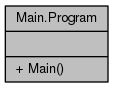
\includegraphics[width=157pt]{class_main_1_1_program__coll__graph}
\end{center}
\end{figure}
\subsection*{Static Public Member Functions}
\begin{DoxyCompactItemize}
\item 
static void \hyperlink{class_main_1_1_program_a12e5ed1a2cfec9879a107cbd1deaaecf}{Main} (string\mbox{[}$\,$\mbox{]} args)
\end{DoxyCompactItemize}


\subsection{Detailed Description}


Definition at line 19 of file Program.\+cs.



\subsection{Member Function Documentation}
\index{Main\+::\+Program@{Main\+::\+Program}!Main@{Main}}
\index{Main@{Main}!Main\+::\+Program@{Main\+::\+Program}}
\subsubsection[{\texorpdfstring{Main(string[] args)}{Main(string[] args)}}]{\setlength{\rightskip}{0pt plus 5cm}static void Main.\+Program.\+Main (
\begin{DoxyParamCaption}
\item[{string\mbox{[}$\,$\mbox{]}}]{args}
\end{DoxyParamCaption}
)\hspace{0.3cm}{\ttfamily [static]}}\hypertarget{class_main_1_1_program_a12e5ed1a2cfec9879a107cbd1deaaecf}{}\label{class_main_1_1_program_a12e5ed1a2cfec9879a107cbd1deaaecf}


Definition at line 21 of file Program.\+cs.



References Client.\+D\+B\+Client.\+Connect\+To\+Collection(), Data.\+A\+P\+I\+Args.\+Get\+Args(), Services.\+Token.\+Token\+Information.\+Get\+O\+Auth\+Token, Services.\+Proxy.\+Proxy\+Information.\+Get\+Proxy\+Credentials, Services.\+Proxy.\+Proxy\+Information.\+Set\+Value(), and Services.\+Token.\+Token\+Information.\+Set\+Value().



Here is the call graph for this function\+:
\nopagebreak
\begin{figure}[H]
\begin{center}
\leavevmode
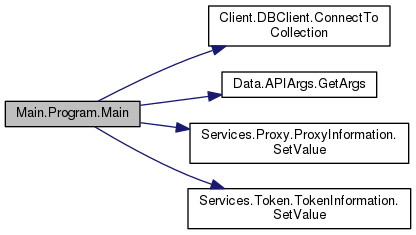
\includegraphics[width=350pt]{class_main_1_1_program_a12e5ed1a2cfec9879a107cbd1deaaecf_cgraph}
\end{center}
\end{figure}




The documentation for this class was generated from the following file\+:\begin{DoxyCompactItemize}
\item 
Facebook\+Application/\+Main/\hyperlink{_main_2_program_8cs}{Program.\+cs}\end{DoxyCompactItemize}

\hypertarget{class_data_1_1_facebook_objects_1_1_properties}{}\section{Data.\+Facebook\+Objects.\+Properties Class Reference}
\label{class_data_1_1_facebook_objects_1_1_properties}\index{Data.\+Facebook\+Objects.\+Properties@{Data.\+Facebook\+Objects.\+Properties}}


Collaboration diagram for Data.\+Facebook\+Objects.\+Properties\+:
\nopagebreak
\begin{figure}[H]
\begin{center}
\leavevmode
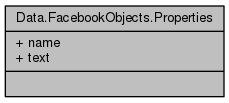
\includegraphics[width=244pt]{class_data_1_1_facebook_objects_1_1_properties__coll__graph}
\end{center}
\end{figure}
\subsection*{Properties}
\begin{DoxyCompactItemize}
\item 
string \hyperlink{class_data_1_1_facebook_objects_1_1_properties_a530a5e9d4bc85426eefe154d5ef069f9}{name}\hspace{0.3cm}{\ttfamily  \mbox{[}get, set\mbox{]}}
\item 
string \hyperlink{class_data_1_1_facebook_objects_1_1_properties_aed35ce8968a53f6250ad88398e4218b1}{text}\hspace{0.3cm}{\ttfamily  \mbox{[}get, set\mbox{]}}
\end{DoxyCompactItemize}


\subsection{Detailed Description}


Definition at line 21 of file Post.\+cs.



\subsection{Property Documentation}
\index{Data\+::\+Facebook\+Objects\+::\+Properties@{Data\+::\+Facebook\+Objects\+::\+Properties}!name@{name}}
\index{name@{name}!Data\+::\+Facebook\+Objects\+::\+Properties@{Data\+::\+Facebook\+Objects\+::\+Properties}}
\subsubsection[{\texorpdfstring{name}{name}}]{\setlength{\rightskip}{0pt plus 5cm}string Data.\+Facebook\+Objects.\+Properties.\+name\hspace{0.3cm}{\ttfamily [get]}, {\ttfamily [set]}}\hypertarget{class_data_1_1_facebook_objects_1_1_properties_a530a5e9d4bc85426eefe154d5ef069f9}{}\label{class_data_1_1_facebook_objects_1_1_properties_a530a5e9d4bc85426eefe154d5ef069f9}


Definition at line 23 of file Post.\+cs.

\index{Data\+::\+Facebook\+Objects\+::\+Properties@{Data\+::\+Facebook\+Objects\+::\+Properties}!text@{text}}
\index{text@{text}!Data\+::\+Facebook\+Objects\+::\+Properties@{Data\+::\+Facebook\+Objects\+::\+Properties}}
\subsubsection[{\texorpdfstring{text}{text}}]{\setlength{\rightskip}{0pt plus 5cm}string Data.\+Facebook\+Objects.\+Properties.\+text\hspace{0.3cm}{\ttfamily [get]}, {\ttfamily [set]}}\hypertarget{class_data_1_1_facebook_objects_1_1_properties_aed35ce8968a53f6250ad88398e4218b1}{}\label{class_data_1_1_facebook_objects_1_1_properties_aed35ce8968a53f6250ad88398e4218b1}


Definition at line 24 of file Post.\+cs.



The documentation for this class was generated from the following file\+:\begin{DoxyCompactItemize}
\item 
Facebook\+Application/\+Data/\+Facebook\+Objects/\hyperlink{_post_8cs}{Post.\+cs}\end{DoxyCompactItemize}

\hypertarget{class_services_1_1_proxy_1_1_proxy_information}{}\section{Services.\+Proxy.\+Proxy\+Information Class Reference}
\label{class_services_1_1_proxy_1_1_proxy_information}\index{Services.\+Proxy.\+Proxy\+Information@{Services.\+Proxy.\+Proxy\+Information}}


Inheritance diagram for Services.\+Proxy.\+Proxy\+Information\+:
\nopagebreak
\begin{figure}[H]
\begin{center}
\leavevmode
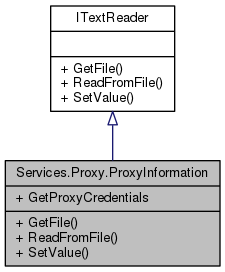
\includegraphics[width=241pt]{class_services_1_1_proxy_1_1_proxy_information__inherit__graph}
\end{center}
\end{figure}


Collaboration diagram for Services.\+Proxy.\+Proxy\+Information\+:
\nopagebreak
\begin{figure}[H]
\begin{center}
\leavevmode
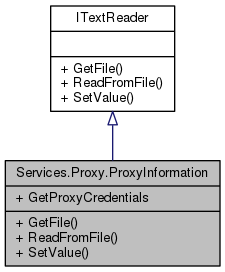
\includegraphics[width=241pt]{class_services_1_1_proxy_1_1_proxy_information__coll__graph}
\end{center}
\end{figure}
\subsection*{Public Member Functions}
\begin{DoxyCompactItemize}
\item 
string\mbox{[}$\,$\mbox{]} \hyperlink{class_services_1_1_proxy_1_1_proxy_information_ac775377976e6b9a38de042bf29440174}{Get\+File} ()
\begin{DoxyCompactList}\small\item\em Identify path to token file. Method to be used as submethod -\/ therefore private scope. \end{DoxyCompactList}\item 
void \hyperlink{class_services_1_1_proxy_1_1_proxy_information_abb9b80a08af3fd6458a68ad258113664}{Read\+From\+File} (Text\+Reader reader)
\begin{DoxyCompactList}\small\item\em Read relevant content from file \end{DoxyCompactList}\item 
void \hyperlink{class_services_1_1_proxy_1_1_proxy_information_aff83ebf7729262cfe2840c26a9ef73f0}{Set\+Value} ()
\begin{DoxyCompactList}\small\item\em Makes the value accessible \end{DoxyCompactList}\end{DoxyCompactItemize}
\subsection*{Properties}
\begin{DoxyCompactItemize}
\item 
Tuple$<$ string, string $>$ \hyperlink{class_services_1_1_proxy_1_1_proxy_information_a618dc0f74995fb57440293d34b4e7019}{Get\+Proxy\+Credentials}\hspace{0.3cm}{\ttfamily  \mbox{[}get\mbox{]}}
\begin{DoxyCompactList}\small\item\em Enables other classes/projects to retrieve the token \end{DoxyCompactList}\end{DoxyCompactItemize}


\subsection{Detailed Description}


Definition at line 7 of file Proxy\+Information.\+cs.



\subsection{Member Function Documentation}
\index{Services\+::\+Proxy\+::\+Proxy\+Information@{Services\+::\+Proxy\+::\+Proxy\+Information}!Get\+File@{Get\+File}}
\index{Get\+File@{Get\+File}!Services\+::\+Proxy\+::\+Proxy\+Information@{Services\+::\+Proxy\+::\+Proxy\+Information}}
\subsubsection[{\texorpdfstring{Get\+File()}{GetFile()}}]{\setlength{\rightskip}{0pt plus 5cm}string \mbox{[}$\,$\mbox{]} Services.\+Proxy.\+Proxy\+Information.\+Get\+File (
\begin{DoxyParamCaption}
{}
\end{DoxyParamCaption}
)}\hypertarget{class_services_1_1_proxy_1_1_proxy_information_ac775377976e6b9a38de042bf29440174}{}\label{class_services_1_1_proxy_1_1_proxy_information_ac775377976e6b9a38de042bf29440174}


Identify path to token file. Method to be used as submethod -\/ therefore private scope. 



Implements \hyperlink{interface_services_1_1_i_text_reader_a729359f5178930c633a7d0480041638a}{Services.\+I\+Text\+Reader}.



Definition at line 17 of file Proxy\+Information.\+cs.

\index{Services\+::\+Proxy\+::\+Proxy\+Information@{Services\+::\+Proxy\+::\+Proxy\+Information}!Read\+From\+File@{Read\+From\+File}}
\index{Read\+From\+File@{Read\+From\+File}!Services\+::\+Proxy\+::\+Proxy\+Information@{Services\+::\+Proxy\+::\+Proxy\+Information}}
\subsubsection[{\texorpdfstring{Read\+From\+File(\+Text\+Reader reader)}{ReadFromFile(TextReader reader)}}]{\setlength{\rightskip}{0pt plus 5cm}void Services.\+Proxy.\+Proxy\+Information.\+Read\+From\+File (
\begin{DoxyParamCaption}
\item[{Text\+Reader}]{reader}
\end{DoxyParamCaption}
)}\hypertarget{class_services_1_1_proxy_1_1_proxy_information_abb9b80a08af3fd6458a68ad258113664}{}\label{class_services_1_1_proxy_1_1_proxy_information_abb9b80a08af3fd6458a68ad258113664}


Read relevant content from file 


\begin{DoxyParams}{Parameters}
{\em reader} & Text\+Reader Objecet.\\
\hline
\end{DoxyParams}


Implements \hyperlink{interface_services_1_1_i_text_reader_ab635d59d4de79bf41ffe7a184473f416}{Services.\+I\+Text\+Reader}.



Definition at line 36 of file Proxy\+Information.\+cs.

\index{Services\+::\+Proxy\+::\+Proxy\+Information@{Services\+::\+Proxy\+::\+Proxy\+Information}!Set\+Value@{Set\+Value}}
\index{Set\+Value@{Set\+Value}!Services\+::\+Proxy\+::\+Proxy\+Information@{Services\+::\+Proxy\+::\+Proxy\+Information}}
\subsubsection[{\texorpdfstring{Set\+Value()}{SetValue()}}]{\setlength{\rightskip}{0pt plus 5cm}void Services.\+Proxy.\+Proxy\+Information.\+Set\+Value (
\begin{DoxyParamCaption}
{}
\end{DoxyParamCaption}
)}\hypertarget{class_services_1_1_proxy_1_1_proxy_information_aff83ebf7729262cfe2840c26a9ef73f0}{}\label{class_services_1_1_proxy_1_1_proxy_information_aff83ebf7729262cfe2840c26a9ef73f0}


Makes the value accessible 



Implements \hyperlink{interface_services_1_1_i_text_reader_a670edc32225de1bcaf9942b4acc1edaf}{Services.\+I\+Text\+Reader}.



Definition at line 42 of file Proxy\+Information.\+cs.



Referenced by Main.\+Program.\+Main().



Here is the caller graph for this function\+:
\nopagebreak
\begin{figure}[H]
\begin{center}
\leavevmode
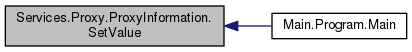
\includegraphics[width=350pt]{class_services_1_1_proxy_1_1_proxy_information_aff83ebf7729262cfe2840c26a9ef73f0_icgraph}
\end{center}
\end{figure}




\subsection{Property Documentation}
\index{Services\+::\+Proxy\+::\+Proxy\+Information@{Services\+::\+Proxy\+::\+Proxy\+Information}!Get\+Proxy\+Credentials@{Get\+Proxy\+Credentials}}
\index{Get\+Proxy\+Credentials@{Get\+Proxy\+Credentials}!Services\+::\+Proxy\+::\+Proxy\+Information@{Services\+::\+Proxy\+::\+Proxy\+Information}}
\subsubsection[{\texorpdfstring{Get\+Proxy\+Credentials}{GetProxyCredentials}}]{\setlength{\rightskip}{0pt plus 5cm}Tuple$<$string, string$>$ Services.\+Proxy.\+Proxy\+Information.\+Get\+Proxy\+Credentials\hspace{0.3cm}{\ttfamily [get]}}\hypertarget{class_services_1_1_proxy_1_1_proxy_information_a618dc0f74995fb57440293d34b4e7019}{}\label{class_services_1_1_proxy_1_1_proxy_information_a618dc0f74995fb57440293d34b4e7019}


Enables other classes/projects to retrieve the token 

Facebook O\+Auth \hyperlink{namespace_services_1_1_token}{Token}

Definition at line 57 of file Proxy\+Information.\+cs.



Referenced by Main.\+Program.\+Main().



The documentation for this class was generated from the following file\+:\begin{DoxyCompactItemize}
\item 
Facebook\+Application/\+Services/\+Proxy/\hyperlink{_proxy_information_8cs}{Proxy\+Information.\+cs}\end{DoxyCompactItemize}

\hypertarget{class_services_1_1_token_1_1_token_information}{}\section{Services.\+Token.\+Token\+Information Class Reference}
\label{class_services_1_1_token_1_1_token_information}\index{Services.\+Token.\+Token\+Information@{Services.\+Token.\+Token\+Information}}


Inheritance diagram for Services.\+Token.\+Token\+Information\+:
\nopagebreak
\begin{figure}[H]
\begin{center}
\leavevmode
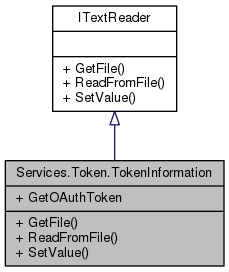
\includegraphics[width=244pt]{class_services_1_1_token_1_1_token_information__inherit__graph}
\end{center}
\end{figure}


Collaboration diagram for Services.\+Token.\+Token\+Information\+:
\nopagebreak
\begin{figure}[H]
\begin{center}
\leavevmode
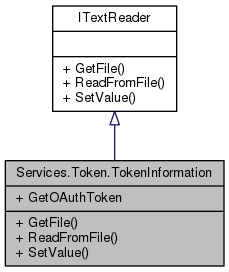
\includegraphics[width=244pt]{class_services_1_1_token_1_1_token_information__coll__graph}
\end{center}
\end{figure}
\subsection*{Public Member Functions}
\begin{DoxyCompactItemize}
\item 
string\mbox{[}$\,$\mbox{]} \hyperlink{class_services_1_1_token_1_1_token_information_a37295436ba6b0c749486fcb647fcd904}{Get\+File} ()
\begin{DoxyCompactList}\small\item\em Identify path to token file. Method to be used as submethod -\/ therefore private scope. \end{DoxyCompactList}\item 
void \hyperlink{class_services_1_1_token_1_1_token_information_ac080b926c4adadd033ebad6cea64baf4}{Read\+From\+File} (Text\+Reader reader)
\begin{DoxyCompactList}\small\item\em Reads a whatever is provided by a Text\+Reader stream object and writes to the private private\+Token \end{DoxyCompactList}\item 
void \hyperlink{class_services_1_1_token_1_1_token_information_a2cdb068d0ace07409c398e3c40c5b84d}{Set\+Value} ()
\begin{DoxyCompactList}\small\item\em Provides a Text\+Reader stream to the Read\+Token()-\/method. \end{DoxyCompactList}\end{DoxyCompactItemize}
\subsection*{Properties}
\begin{DoxyCompactItemize}
\item 
string \hyperlink{class_services_1_1_token_1_1_token_information_a553143fafe504da889f94942961ceb41}{Get\+O\+Auth\+Token}\hspace{0.3cm}{\ttfamily  \mbox{[}get\mbox{]}}
\begin{DoxyCompactList}\small\item\em Enables other classes/projects to retrieve the token \end{DoxyCompactList}\end{DoxyCompactItemize}


\subsection{Detailed Description}


Definition at line 6 of file Token\+Information.\+cs.



\subsection{Member Function Documentation}
\index{Services\+::\+Token\+::\+Token\+Information@{Services\+::\+Token\+::\+Token\+Information}!Get\+File@{Get\+File}}
\index{Get\+File@{Get\+File}!Services\+::\+Token\+::\+Token\+Information@{Services\+::\+Token\+::\+Token\+Information}}
\subsubsection[{\texorpdfstring{Get\+File()}{GetFile()}}]{\setlength{\rightskip}{0pt plus 5cm}string \mbox{[}$\,$\mbox{]} Services.\+Token.\+Token\+Information.\+Get\+File (
\begin{DoxyParamCaption}
{}
\end{DoxyParamCaption}
)}\hypertarget{class_services_1_1_token_1_1_token_information_a37295436ba6b0c749486fcb647fcd904}{}\label{class_services_1_1_token_1_1_token_information_a37295436ba6b0c749486fcb647fcd904}


Identify path to token file. Method to be used as submethod -\/ therefore private scope. 

\begin{DoxyReturn}{Returns}
A path to the token-\/file
\end{DoxyReturn}


Implements \hyperlink{interface_services_1_1_i_text_reader_a729359f5178930c633a7d0480041638a}{Services.\+I\+Text\+Reader}.



Definition at line 19 of file Token\+Information.\+cs.

\index{Services\+::\+Token\+::\+Token\+Information@{Services\+::\+Token\+::\+Token\+Information}!Read\+From\+File@{Read\+From\+File}}
\index{Read\+From\+File@{Read\+From\+File}!Services\+::\+Token\+::\+Token\+Information@{Services\+::\+Token\+::\+Token\+Information}}
\subsubsection[{\texorpdfstring{Read\+From\+File(\+Text\+Reader reader)}{ReadFromFile(TextReader reader)}}]{\setlength{\rightskip}{0pt plus 5cm}void Services.\+Token.\+Token\+Information.\+Read\+From\+File (
\begin{DoxyParamCaption}
\item[{Text\+Reader}]{reader}
\end{DoxyParamCaption}
)}\hypertarget{class_services_1_1_token_1_1_token_information_ac080b926c4adadd033ebad6cea64baf4}{}\label{class_services_1_1_token_1_1_token_information_ac080b926c4adadd033ebad6cea64baf4}


Reads a whatever is provided by a Text\+Reader stream object and writes to the private private\+Token 


\begin{DoxyParams}{Parameters}
{\em reader} & Text\+Reader object -\/ here a p.\\
\hline
\end{DoxyParams}


Implements \hyperlink{interface_services_1_1_i_text_reader_ab635d59d4de79bf41ffe7a184473f416}{Services.\+I\+Text\+Reader}.



Definition at line 42 of file Token\+Information.\+cs.

\index{Services\+::\+Token\+::\+Token\+Information@{Services\+::\+Token\+::\+Token\+Information}!Set\+Value@{Set\+Value}}
\index{Set\+Value@{Set\+Value}!Services\+::\+Token\+::\+Token\+Information@{Services\+::\+Token\+::\+Token\+Information}}
\subsubsection[{\texorpdfstring{Set\+Value()}{SetValue()}}]{\setlength{\rightskip}{0pt plus 5cm}void Services.\+Token.\+Token\+Information.\+Set\+Value (
\begin{DoxyParamCaption}
{}
\end{DoxyParamCaption}
)}\hypertarget{class_services_1_1_token_1_1_token_information_a2cdb068d0ace07409c398e3c40c5b84d}{}\label{class_services_1_1_token_1_1_token_information_a2cdb068d0ace07409c398e3c40c5b84d}


Provides a Text\+Reader stream to the Read\+Token()-\/method. 



Implements \hyperlink{interface_services_1_1_i_text_reader_a670edc32225de1bcaf9942b4acc1edaf}{Services.\+I\+Text\+Reader}.



Definition at line 51 of file Token\+Information.\+cs.



Referenced by Main.\+Program.\+Main().



Here is the caller graph for this function\+:
\nopagebreak
\begin{figure}[H]
\begin{center}
\leavevmode
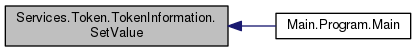
\includegraphics[width=350pt]{class_services_1_1_token_1_1_token_information_a2cdb068d0ace07409c398e3c40c5b84d_icgraph}
\end{center}
\end{figure}




\subsection{Property Documentation}
\index{Services\+::\+Token\+::\+Token\+Information@{Services\+::\+Token\+::\+Token\+Information}!Get\+O\+Auth\+Token@{Get\+O\+Auth\+Token}}
\index{Get\+O\+Auth\+Token@{Get\+O\+Auth\+Token}!Services\+::\+Token\+::\+Token\+Information@{Services\+::\+Token\+::\+Token\+Information}}
\subsubsection[{\texorpdfstring{Get\+O\+Auth\+Token}{GetOAuthToken}}]{\setlength{\rightskip}{0pt plus 5cm}string Services.\+Token.\+Token\+Information.\+Get\+O\+Auth\+Token\hspace{0.3cm}{\ttfamily [get]}}\hypertarget{class_services_1_1_token_1_1_token_information_a553143fafe504da889f94942961ceb41}{}\label{class_services_1_1_token_1_1_token_information_a553143fafe504da889f94942961ceb41}


Enables other classes/projects to retrieve the token 

Facebook O\+Auth \hyperlink{namespace_services_1_1_token}{Token}

Definition at line 66 of file Token\+Information.\+cs.



Referenced by Main.\+Program.\+Main().



The documentation for this class was generated from the following file\+:\begin{DoxyCompactItemize}
\item 
Facebook\+Application/\+Services/\+Token/\hyperlink{_token_information_8cs}{Token\+Information.\+cs}\end{DoxyCompactItemize}

\chapter{File Documentation}
\hypertarget{_d_b_client_8cs}{}\section{Facebook\+Application/\+Client/\+D\+B\+Client.cs File Reference}
\label{_d_b_client_8cs}\index{Facebook\+Application/\+Client/\+D\+B\+Client.\+cs@{Facebook\+Application/\+Client/\+D\+B\+Client.\+cs}}
\subsection*{Classes}
\begin{DoxyCompactItemize}
\item 
interface \hyperlink{interface_client_1_1_i_d_b_client}{Client.\+I\+D\+B\+Client}
\item 
class \hyperlink{class_client_1_1_d_b_client}{Client.\+D\+B\+Client}
\end{DoxyCompactItemize}
\subsection*{Namespaces}
\begin{DoxyCompactItemize}
\item 
namespace \hyperlink{namespace_client}{Client}
\end{DoxyCompactItemize}

\hypertarget{_facebook_client_8cs}{}\section{Facebook\+Application/\+Client/\+Facebook\+Client.cs File Reference}
\label{_facebook_client_8cs}\index{Facebook\+Application/\+Client/\+Facebook\+Client.\+cs@{Facebook\+Application/\+Client/\+Facebook\+Client.\+cs}}
\subsection*{Classes}
\begin{DoxyCompactItemize}
\item 
interface \hyperlink{interface_client_1_1_i_facebook_client}{Client.\+I\+Facebook\+Client}
\begin{DoxyCompactList}\small\item\em Interface Framework for \hyperlink{class_client_1_1_facebook_client}{Facebook\+Client} \end{DoxyCompactList}\item 
class \hyperlink{class_client_1_1_facebook_client}{Client.\+Facebook\+Client}
\begin{DoxyCompactList}\small\item\em \hyperlink{class_client_1_1_facebook_client}{Facebook\+Client} Class \end{DoxyCompactList}\end{DoxyCompactItemize}
\subsection*{Namespaces}
\begin{DoxyCompactItemize}
\item 
namespace \hyperlink{namespace_client}{Client}
\end{DoxyCompactItemize}

\hypertarget{_client_2_properties_2_assembly_info_8cs}{}\section{Facebook\+Application/\+Client/\+Properties/\+Assembly\+Info.cs File Reference}
\label{_client_2_properties_2_assembly_info_8cs}\index{Facebook\+Application/\+Client/\+Properties/\+Assembly\+Info.\+cs@{Facebook\+Application/\+Client/\+Properties/\+Assembly\+Info.\+cs}}

\hypertarget{_data_2_properties_2_assembly_info_8cs}{}\section{Facebook\+Application/\+Data/\+Properties/\+Assembly\+Info.cs File Reference}
\label{_data_2_properties_2_assembly_info_8cs}\index{Facebook\+Application/\+Data/\+Properties/\+Assembly\+Info.\+cs@{Facebook\+Application/\+Data/\+Properties/\+Assembly\+Info.\+cs}}

\hypertarget{_g_u_i_2_properties_2_assembly_info_8cs}{}\section{Facebook\+Application/\+G\+U\+I/\+Properties/\+Assembly\+Info.cs File Reference}
\label{_g_u_i_2_properties_2_assembly_info_8cs}\index{Facebook\+Application/\+G\+U\+I/\+Properties/\+Assembly\+Info.\+cs@{Facebook\+Application/\+G\+U\+I/\+Properties/\+Assembly\+Info.\+cs}}

\hypertarget{_operations_2_properties_2_assembly_info_8cs}{}\section{Facebook\+Application/\+Operations/\+Properties/\+Assembly\+Info.cs File Reference}
\label{_operations_2_properties_2_assembly_info_8cs}\index{Facebook\+Application/\+Operations/\+Properties/\+Assembly\+Info.\+cs@{Facebook\+Application/\+Operations/\+Properties/\+Assembly\+Info.\+cs}}

\hypertarget{_services_2_properties_2_assembly_info_8cs}{}\section{Facebook\+Application/\+Services/\+Properties/\+Assembly\+Info.cs File Reference}
\label{_services_2_properties_2_assembly_info_8cs}\index{Facebook\+Application/\+Services/\+Properties/\+Assembly\+Info.\+cs@{Facebook\+Application/\+Services/\+Properties/\+Assembly\+Info.\+cs}}

\hypertarget{_a_p_i_args_8cs}{}\section{Facebook\+Application/\+Data/\+A\+P\+I\+Args.cs File Reference}
\label{_a_p_i_args_8cs}\index{Facebook\+Application/\+Data/\+A\+P\+I\+Args.\+cs@{Facebook\+Application/\+Data/\+A\+P\+I\+Args.\+cs}}
\subsection*{Classes}
\begin{DoxyCompactItemize}
\item 
class \hyperlink{class_data_1_1_a_p_i_args}{Data.\+A\+P\+I\+Args}
\end{DoxyCompactItemize}
\subsection*{Namespaces}
\begin{DoxyCompactItemize}
\item 
namespace \hyperlink{namespace_data}{Data}
\end{DoxyCompactItemize}

\hypertarget{_comment_8cs}{}\section{Facebook\+Application/\+Data/\+Facebook\+Objects/\+Comment.cs File Reference}
\label{_comment_8cs}\index{Facebook\+Application/\+Data/\+Facebook\+Objects/\+Comment.\+cs@{Facebook\+Application/\+Data/\+Facebook\+Objects/\+Comment.\+cs}}
\subsection*{Classes}
\begin{DoxyCompactItemize}
\item 
class \hyperlink{class_data_1_1_facebook_objects_1_1_comment}{Data.\+Facebook\+Objects.\+Comment}
\item 
class \hyperlink{class_data_1_1_facebook_objects_1_1_application}{Data.\+Facebook\+Objects.\+Application}
\end{DoxyCompactItemize}
\subsection*{Namespaces}
\begin{DoxyCompactItemize}
\item 
namespace \hyperlink{namespace_data_1_1_facebook_objects}{Data.\+Facebook\+Objects}
\end{DoxyCompactItemize}

\hypertarget{_feed_8cs}{}\section{Facebook\+Application/\+Data/\+Facebook\+Objects/\+Feed.cs File Reference}
\label{_feed_8cs}\index{Facebook\+Application/\+Data/\+Facebook\+Objects/\+Feed.\+cs@{Facebook\+Application/\+Data/\+Facebook\+Objects/\+Feed.\+cs}}
\subsection*{Classes}
\begin{DoxyCompactItemize}
\item 
class \hyperlink{class_data_1_1_facebook_objects_1_1_feed}{Data.\+Facebook\+Objects.\+Feed}
\end{DoxyCompactItemize}
\subsection*{Namespaces}
\begin{DoxyCompactItemize}
\item 
namespace \hyperlink{namespace_data_1_1_facebook_objects}{Data.\+Facebook\+Objects}
\end{DoxyCompactItemize}

\hypertarget{_post_8cs}{}\section{Facebook\+Application/\+Data/\+Facebook\+Objects/\+Post.cs File Reference}
\label{_post_8cs}\index{Facebook\+Application/\+Data/\+Facebook\+Objects/\+Post.\+cs@{Facebook\+Application/\+Data/\+Facebook\+Objects/\+Post.\+cs}}
\subsection*{Classes}
\begin{DoxyCompactItemize}
\item 
class \hyperlink{class_data_1_1_facebook_objects_1_1_post}{Data.\+Facebook\+Objects.\+Post}
\item 
class \hyperlink{class_data_1_1_facebook_objects_1_1_properties}{Data.\+Facebook\+Objects.\+Properties}
\end{DoxyCompactItemize}
\subsection*{Namespaces}
\begin{DoxyCompactItemize}
\item 
namespace \hyperlink{namespace_data_1_1_facebook_objects}{Data.\+Facebook\+Objects}
\end{DoxyCompactItemize}

\hypertarget{generated_8cs}{}\section{Facebook\+Application/\+G\+U\+I/gtk-\/gui/generated.cs File Reference}
\label{generated_8cs}\index{Facebook\+Application/\+G\+U\+I/gtk-\/gui/generated.\+cs@{Facebook\+Application/\+G\+U\+I/gtk-\/gui/generated.\+cs}}
\subsection*{Classes}
\begin{DoxyCompactItemize}
\item 
class {\bfseries Stetic.\+Gui}
\item 
class {\bfseries Stetic.\+Action\+Groups}
\end{DoxyCompactItemize}
\subsection*{Namespaces}
\begin{DoxyCompactItemize}
\item 
namespace \hyperlink{namespace_stetic}{Stetic}
\end{DoxyCompactItemize}

\hypertarget{gtk-gui_2_main_window_8cs}{}\section{Facebook\+Application/\+G\+U\+I/gtk-\/gui/\+Main\+Window.cs File Reference}
\label{gtk-gui_2_main_window_8cs}\index{Facebook\+Application/\+G\+U\+I/gtk-\/gui/\+Main\+Window.\+cs@{Facebook\+Application/\+G\+U\+I/gtk-\/gui/\+Main\+Window.\+cs}}
\subsection*{Classes}
\begin{DoxyCompactItemize}
\item 
class \hyperlink{class_main_window}{Main\+Window}
\end{DoxyCompactItemize}

\hypertarget{_main_window_8cs}{}\section{Facebook\+Application/\+G\+U\+I/\+Main\+Window.cs File Reference}
\label{_main_window_8cs}\index{Facebook\+Application/\+G\+U\+I/\+Main\+Window.\+cs@{Facebook\+Application/\+G\+U\+I/\+Main\+Window.\+cs}}
\subsection*{Classes}
\begin{DoxyCompactItemize}
\item 
class \hyperlink{class_main_window}{Main\+Window}
\end{DoxyCompactItemize}

\hypertarget{_g_u_i_2_program_8cs}{}\section{Facebook\+Application/\+G\+U\+I/\+Program.cs File Reference}
\label{_g_u_i_2_program_8cs}\index{Facebook\+Application/\+G\+U\+I/\+Program.\+cs@{Facebook\+Application/\+G\+U\+I/\+Program.\+cs}}
\subsection*{Classes}
\begin{DoxyCompactItemize}
\item 
class \hyperlink{class_g_u_i_1_1_main_class}{G\+U\+I.\+Main\+Class}
\end{DoxyCompactItemize}
\subsection*{Namespaces}
\begin{DoxyCompactItemize}
\item 
namespace \hyperlink{namespace_g_u_i}{G\+UI}
\end{DoxyCompactItemize}

\hypertarget{_main_2_program_8cs}{}\section{Facebook\+Application/\+Main/\+Program.cs File Reference}
\label{_main_2_program_8cs}\index{Facebook\+Application/\+Main/\+Program.\+cs@{Facebook\+Application/\+Main/\+Program.\+cs}}
\subsection*{Classes}
\begin{DoxyCompactItemize}
\item 
class \hyperlink{class_main_1_1_program}{Main.\+Program}
\end{DoxyCompactItemize}
\subsection*{Namespaces}
\begin{DoxyCompactItemize}
\item 
namespace \hyperlink{namespace_main}{Main}
\end{DoxyCompactItemize}

\hypertarget{_client_get_operation_8cs}{}\section{Facebook\+Application/\+Operations/\+Client\+Operations/\+Client\+Get\+Operation.cs File Reference}
\label{_client_get_operation_8cs}\index{Facebook\+Application/\+Operations/\+Client\+Operations/\+Client\+Get\+Operation.\+cs@{Facebook\+Application/\+Operations/\+Client\+Operations/\+Client\+Get\+Operation.\+cs}}
\subsection*{Classes}
\begin{DoxyCompactItemize}
\item 
interface \hyperlink{interface_operations_1_1_client_operations_1_1_i_client_get_operations}{Operations.\+Client\+Operations.\+I\+Client\+Get\+Operations}
\item 
class \hyperlink{class_operations_1_1_client_operations_1_1_client_get_operations}{Operations.\+Client\+Operations.\+Client\+Get\+Operations}
\end{DoxyCompactItemize}
\subsection*{Namespaces}
\begin{DoxyCompactItemize}
\item 
namespace \hyperlink{namespace_operations_1_1_client_operations}{Operations.\+Client\+Operations}
\end{DoxyCompactItemize}

\hypertarget{_client_store_operations_8cs}{}\section{Facebook\+Application/\+Operations/\+Client\+Operations/\+Client\+Store\+Operations.cs File Reference}
\label{_client_store_operations_8cs}\index{Facebook\+Application/\+Operations/\+Client\+Operations/\+Client\+Store\+Operations.\+cs@{Facebook\+Application/\+Operations/\+Client\+Operations/\+Client\+Store\+Operations.\+cs}}
\subsection*{Classes}
\begin{DoxyCompactItemize}
\item 
interface \hyperlink{interface_operations_1_1_client_operations_1_1_i_client_store_operations}{Operations.\+Client\+Operations.\+I\+Client\+Store\+Operations}
\item 
class \hyperlink{class_operations_1_1_client_operations_1_1_client_store_operations}{Operations.\+Client\+Operations.\+Client\+Store\+Operations}
\end{DoxyCompactItemize}
\subsection*{Namespaces}
\begin{DoxyCompactItemize}
\item 
namespace \hyperlink{namespace_operations_1_1_client_operations}{Operations.\+Client\+Operations}
\end{DoxyCompactItemize}

\hypertarget{_populate_n_e_t_object_8cs}{}\section{Facebook\+Application/\+Operations/\+Data\+Operations/\+Populate\+N\+E\+T\+Object.cs File Reference}
\label{_populate_n_e_t_object_8cs}\index{Facebook\+Application/\+Operations/\+Data\+Operations/\+Populate\+N\+E\+T\+Object.\+cs@{Facebook\+Application/\+Operations/\+Data\+Operations/\+Populate\+N\+E\+T\+Object.\+cs}}
\subsection*{Classes}
\begin{DoxyCompactItemize}
\item 
interface \hyperlink{interface_operations_1_1_data_operations_1_1_i_populate_n_e_t_object}{Operations.\+Data\+Operations.\+I\+Populate\+N\+E\+T\+Object}
\item 
class \hyperlink{class_operations_1_1_data_operations_1_1_populate_n_e_t_object}{Operations.\+Data\+Operations.\+Populate\+N\+E\+T\+Object}
\begin{DoxyCompactList}\small\item\em Class with methods for populating custom object-\/types \end{DoxyCompactList}\end{DoxyCompactItemize}
\subsection*{Namespaces}
\begin{DoxyCompactItemize}
\item 
namespace \hyperlink{namespace_operations_1_1_data_operations}{Operations.\+Data\+Operations}
\end{DoxyCompactItemize}

\hypertarget{_l_i_c_e_n_s_e_8md}{}\section{Facebook\+Application/packages/\+Newtonsoft.Json.10.0.3/\+L\+I\+C\+E\+N\+SE.md File Reference}
\label{_l_i_c_e_n_s_e_8md}\index{Facebook\+Application/packages/\+Newtonsoft.\+Json.\+10.\+0.\+3/\+L\+I\+C\+E\+N\+S\+E.\+md@{Facebook\+Application/packages/\+Newtonsoft.\+Json.\+10.\+0.\+3/\+L\+I\+C\+E\+N\+S\+E.\+md}}

\hypertarget{_i_text_reader_8cs}{}\section{Facebook\+Application/\+Services/\+I\+Text\+Reader.cs File Reference}
\label{_i_text_reader_8cs}\index{Facebook\+Application/\+Services/\+I\+Text\+Reader.\+cs@{Facebook\+Application/\+Services/\+I\+Text\+Reader.\+cs}}
\subsection*{Classes}
\begin{DoxyCompactItemize}
\item 
interface \hyperlink{interface_services_1_1_i_text_reader}{Services.\+I\+Text\+Reader}
\end{DoxyCompactItemize}
\subsection*{Namespaces}
\begin{DoxyCompactItemize}
\item 
namespace \hyperlink{namespace_services}{Services}
\end{DoxyCompactItemize}

\hypertarget{_proxy_information_8cs}{}\section{Facebook\+Application/\+Services/\+Proxy/\+Proxy\+Information.cs File Reference}
\label{_proxy_information_8cs}\index{Facebook\+Application/\+Services/\+Proxy/\+Proxy\+Information.\+cs@{Facebook\+Application/\+Services/\+Proxy/\+Proxy\+Information.\+cs}}
\subsection*{Classes}
\begin{DoxyCompactItemize}
\item 
class \hyperlink{class_services_1_1_proxy_1_1_proxy_information}{Services.\+Proxy.\+Proxy\+Information}
\end{DoxyCompactItemize}
\subsection*{Namespaces}
\begin{DoxyCompactItemize}
\item 
namespace \hyperlink{namespace_services_1_1_proxy}{Services.\+Proxy}
\end{DoxyCompactItemize}

\hypertarget{_token_information_8cs}{}\section{Facebook\+Application/\+Services/\+Token/\+Token\+Information.cs File Reference}
\label{_token_information_8cs}\index{Facebook\+Application/\+Services/\+Token/\+Token\+Information.\+cs@{Facebook\+Application/\+Services/\+Token/\+Token\+Information.\+cs}}
\subsection*{Classes}
\begin{DoxyCompactItemize}
\item 
class \hyperlink{class_services_1_1_token_1_1_token_information}{Services.\+Token.\+Token\+Information}
\end{DoxyCompactItemize}
\subsection*{Namespaces}
\begin{DoxyCompactItemize}
\item 
namespace \hyperlink{namespace_services_1_1_token}{Services.\+Token}
\end{DoxyCompactItemize}

%--- End generated contents ---

% Index
\backmatter
\newpage
\phantomsection
\clearemptydoublepage
\addcontentsline{toc}{chapter}{Index}
\printindex

\end{document}
